\documentclass[a4paper, 12pt]{article}
\usepackage[utf8]{inputenc}
\usepackage[T1, T2A]{fontenc}
\usepackage[a4paper, top=2cm, bottom=2cm, left=1cm, right=1cm, marginparwidth=1.75cm]{geometry}
\usepackage{graphicx}
\usepackage{amsmath}
\usepackage{amssymb}
\usepackage{amsfonts}
\usepackage{indentfirst}
\usepackage[english, russian]{babel}
\usepackage[section,above,below]{placeins}
\usepackage{pdfpages} 
\usepackage{svg}
\usepackage[colorlinks,urlcolor=blue]{hyperref}

\newcommand{\V}[1]{\int_Q #1(y) E(x-y) dy}
\newcommand{\R}[1]{\mathbb{R}^#1}
\newcommand{\ro}{ \tilde \rho_N}
\newcommand{\der}[2]{\dfrac{\partial #1}{\partial #2}}
\newtheorem{Lem}{Лемма}

\newenvironment{Proof} % имя окружения
{\par\noindent{\bf Доказательство.}} % команды для \begin
{\hfill$\scriptstyle\blacksquare$} % команды для \end


\begin{document}

\tableofcontents
\newpage

\section*{Введение}
В геофизике существует понятие обратной задачи гравиметрии (ОЗГ) --- нахождении плотности тела по известной информации о потенциале или напряжённости его гравитационного поля, которые могут быть измерены гравиметрами.
В используемых обозначениях $Q$ представляет собой некоторое тело, обладающее гравитационным полем, и требуется найти плотность $\rho$ этого тела,
имея информацию о значении $\varphi$ потенциала поля на некоторой поверхности $S$.
В частности, $Q$ может быть Землёй, $S$ --- некоторым условным шаром, проходящим через вышки для измерения гравитационного поля, а $\varphi$ --- усреднёнными показаниями с вышек, причём ведущую роль играют именно аномальные показания.
Плотность $\rho$ Земли требуется найти для изучения её внутренней структуры и возможности строить предсказания из полученных выводов.
Поиск залежей полезных ископаемых, подземных источников воды, проверка теорий о подземных пустотах как на Земле, так и на Луне, --- всё суть практические примеры использования обратной задачи гравиметрии. 
\begin{figure}[h!]
  \noindent\centering{
  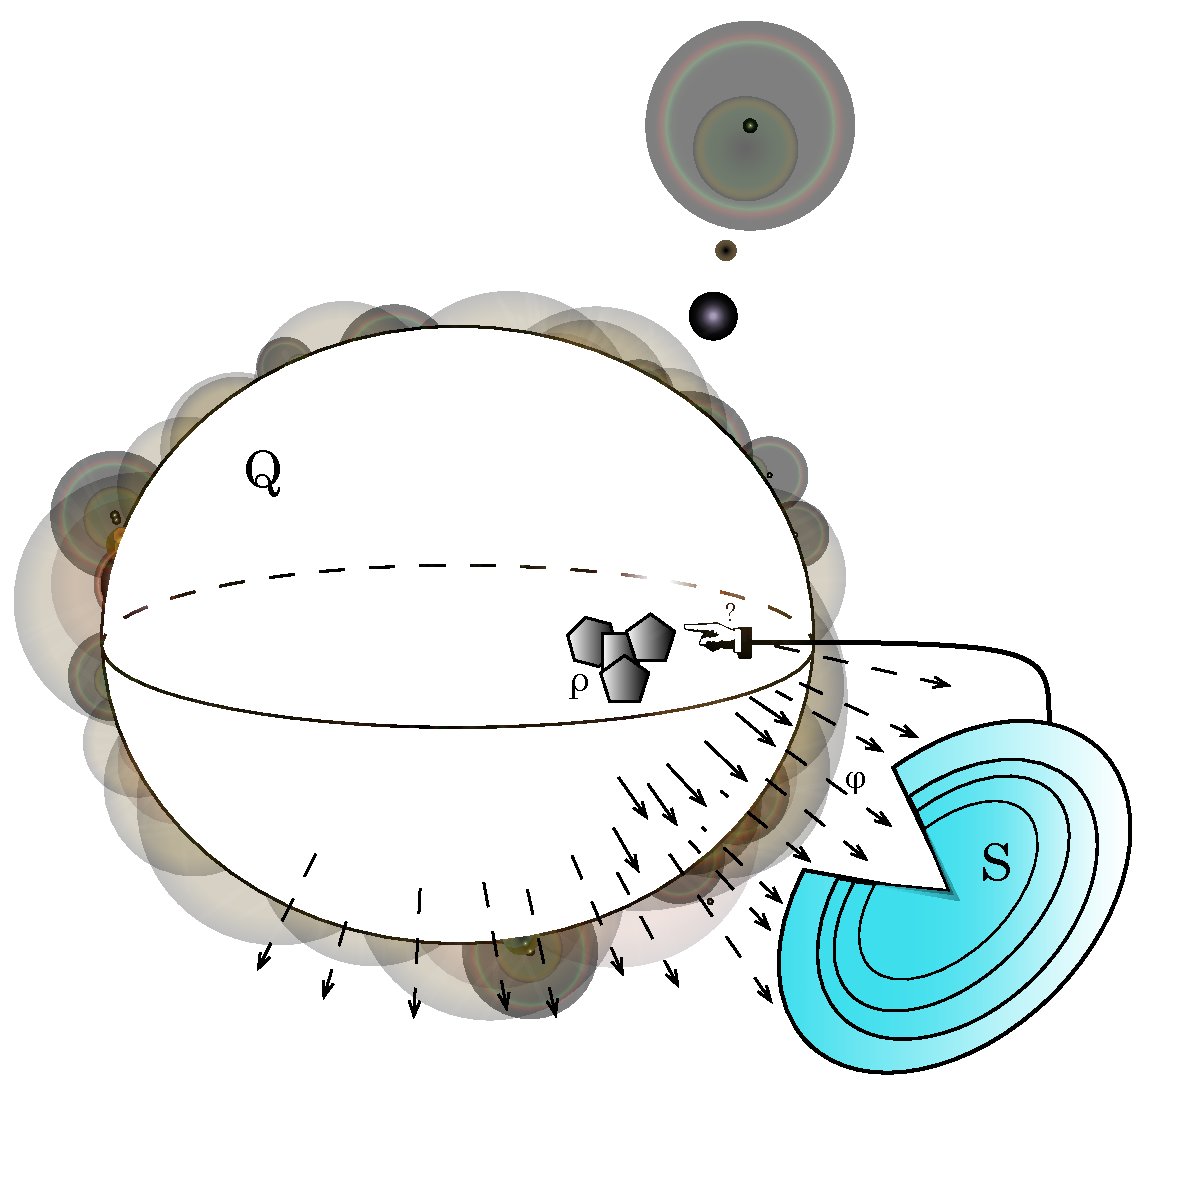
\includegraphics[width=0.9\linewidth]{tit.pdf}
}
  \caption{Геометрия задачи}
  \label{kvci}
  \end{figure} 

При этом возникают вопросы, насколько достоверно мы можем отыскать $\rho$ и какая поверхность $S$ лучше подойдёт для этого (например, как высоко от поверхности Земли лучше вычислять гравитационное поле).
Известно, что ОЗГ не является корректно поставленной, поэтому во многих случаях плотность нельзя достоверно восстановить по характеристикам  порождённого ею поля. 

\section*{Обозначения}
$Q$ --- область в пространстве $\mathbb{R}^n, n\geq 2$, $S$ --- поверхность в том же пространстве,
$\bar Q = Q \bigcup \partial Q$ --- замыкание $Q$,
$Q^+= \R{n}\backslash \bar Q$,
$G(Q)$ --- подпространство гармонических в $L_2(Q)$ функций, $N(Q)$ --- подпространство плотностей нуль-потенциалов в $L_2(Q)$,
$\nabla$ --- градиент,
$\Delta$ --- оператор Лапласа,
$E(x)= -2\pi \ln |x|, x \in Q$ --- фундаментальное решение оператора Лапласа в $\R{2}$,
$\alpha_i=\alpha_i(z)=E(z-z_i)$ --- базисный потенциал, связанный с точкой $z_i \in Q^+$,



\part{Обратная задача гравиметрии (ОЗГ)}

\section{Постановка задачи}
Пусть $Q\subset \R{n}, n=2,3$ --- ограниченная область с ляпуновской границей,
$S \subset \R{n}\backslash Q$ --- достаточно гладкая поверхность (расположенная произвольно относительно $Q$), $\varphi: S \rightarrow \mathbb{R}$ --- действительная функция, заданная на $S$.
Требуется найти плотность $\rho \in L_2(Q) \bigcap G(Q)$ из выражения
\begin{equation}
    \forall x \in S: V_\rho(x)= \V{\rho}= \varphi(x).
\end{equation}

Хорошо известно, что ОЗГ не является однозначно разрешимой, но Новиков П. С. в 1938 г. доказал следующий результат, позволяющий надеяться на частичное решение:
по лемме Новикова (\cite{lezh}, стр. 56, \cite{nov}, стр. 123-126) для любой области $Q$ с ляпуновской границей пространство $L_2(Q)$ раскладывается в прямую сумму 
\begin{equation}
    L_2(Q)= G(Q) \oplus N(Q),
\end{equation}
где $G(Q)$ --- пространство гармонических на $Q$ функций, $N(Q)$ --- пространство всех функций $\psi$, таких что
\begin{equation}
    \V{\psi}=0, \forall x\in Q^+,
\end{equation}
называемое пространством плотностей нуль-потенциалов в $L_2(Q)$.

Описанный результат значит, что $\forall \beta \in L_2(Q) \ \beta = \beta_1 + \beta_2, \beta_1 \in G(Q), \beta_2 \in N(Q)$, $\V{\beta}=\V{\beta_1}$ независимо от $\beta_2$, то есть для любой плотности $\rho$ возможно найти только её гармоническую компоненту.   

\section{Вспомогательные утверждения}
\subsection{Объёмный потенциал и его свойства}

Пусть
$$V_{\rho}(x)=\int_Q \rho(y) E(x-y) dy,$$
$Q$ --- ограниченная область в $\R{2}, x,y \ \in \R{2}, E(x)= -2 \pi \ln|x|, \rho \in L_2(Q)$.

\begin{Lem}
  $\forall x \in \R{2}$ интеграл $V_{\rho}(x)$ сходится в смысле Лебега.
\end{Lem}
\begin{Proof}
  Докажем, что $\forall x \in \R{2}$ функция $E(x-*) \in L_2(Q)$. Достаточно доказать, что $\int_Q E^2 (x-y) dy < +\infty$. $\exists R>0: Q \subset B_R(x)$ -- шар радиуса $R$ с началом в $x$, поскольку $Q$ -- ограничена.
Рассмотрим интеграл 
$$\int_{B_R(x)} E^2(x-y) dy=\int_{B_R(0)}E^2(y)dy=4\pi^2 \int^{2 \pi}_0 \int^R_0 r\ln^2 r dr d\phi.$$
Он конечен, т. к. функция непрерывна. Т. к.
$$\int_Q E^2(x-y)dy \leq \int_{B_R(x)}E^2(x-y)dy,$$
то лемма доказана. Значит, $V_{\rho}(x)$ сходится как скалярное произведение $(\rho, E)$, где $\rho, E \in L_2(Q)$.

\end{Proof}

\begin{Lem}
  $V_{\rho} \in C(\R{2})$
\end{Lem}

\begin{Proof}
  Оттолкнёмся от скалярного произведения и будем доказывать непрерывность $V_{\rho}$ в $x_0 \in \R{2}$:
$$V_{\rho}(x)-V_{\rho}(x_0) \rightarrow 0, x \rightarrow x_0.$$
Рассмотрим 
$$|V_{\rho}(x)-V_{\rho}(x_0)|=\biggl|\int_Q \rho(y) \left(E(x-y)-E(x_0-y) \right)dy\biggl| \leq \text{(по неравнеству Коши-Буняковского)}$$
$$\leq \| \rho\|_{L_2(Q)}\|E(x-*)-E(x_0-*)\|,$$
где $\| \rho\|_{L_2(Q)}$ -- ограничена. 

Представим $E(x)$ как сумму $E(x)= E^1_{\varepsilon} (x)+{E}^2_{\varepsilon}(x)$, где
\[
E^1_{\varepsilon}(x) =
\begin{cases}
E(x), & \text{если $|x|\geq \varepsilon$} \\
\ln \varepsilon, & \text{если $|x|<\varepsilon$}
\end{cases},
E^2_{\varepsilon}(x) =
\begin{cases}
0, & \text{если $|x|\geq \varepsilon$} \\
E(x)-\ln \varepsilon, & \text{если $|x|<\varepsilon$}
\end{cases}.
\]
По одному из свойств нормы:
$$\|E(x-*)-E(x_0-*)\| \leq \|E^1_{\varepsilon}(x-*)-E^1_{\varepsilon}(x_0-*)\|+\|E^2_{\varepsilon}(x-*)\|+\|E^2_{\varepsilon}(x_0-*)\|.$$
Так как $E^1_{\varepsilon}$ непрерывна, первое слагаемое в правой части неравенства стремится к 0 при $x \rightarrow x_0, \forall \varepsilon >0$.
Для $E^2_{\varepsilon}$ имеем оценку:
$$\| E^2_{\varepsilon}(x-*)\| \leq \left(\int_{B_{\varepsilon}(0)}E^2(y) dy \right)^2 \rightarrow 0, \varepsilon \rightarrow 0 \text{ как интеграл Лебега по какой-то теореме}$$
\end{Proof}

\subsection{О единственности решения ОЗГ}
Пусть
$$\{V_{\rho} \in L_2(Q)\}=V \in C(\R{2})$$
\def\MYdef{\mathrel{\stackrel{\rm def}=}}
$$V|_{\delta Q}\MYdef \{V_{\rho}|_{\delta Q}: \rho \in L_2(Q)\}$$
$$V|_{\Gamma}= \{V_{\rho}|_{\Gamma}: \rho \in L_2(Q)\}$$
$$a \in V|_{\delta Q} \simeq b \in V|_{\Gamma}: \exists \rho \in L_2(Q):V|_{\delta Q}=a,V|_{\Gamma}=b$$

Контрпримеры (?):
$$V_0(x)=0, V_1 (x) = |Q|\ln|x|, x \in \R{2} \backslash Q$$

{\bfУтверждение}:
$$V_{\rho}(x)-\int_Q \rho(y) dy E(x) \rightarrow 0, x \rightarrow \infty$$
Доказательство:
\begin{multline}
    1)V_{\rho}(x)-\int_Q \rho(y) dy E(x)=\int_Q \rho(y) (E(x-y)-E(x))dy\\
    2) \sup_{y \in Q}|E(x-y)-E(x)| \leq C \max (\ln(|x|+\text{diam} Q)-\ln|x|,\ln|x|-\ln(|x|-\text{diam} Q)) \rightarrow 0, x \rightarrow \infty
\end{multline}

{\bf Единственность задачи Дирихле в плоском случае (Олейник)}. Eсли
$$\Delta u=0 \text{ в } \R{2}\backslash \bar Q, Q\text{-- ограниченная область в $L_2$ с Ляпуновской границей}$$
$$u \text{ органичена в } \R{2}\backslash Q$$
$$u \in C(\R{2}\backslash Q)$$
$$u|_{\delta Q}=0,$$
то $u=0$ в $\R{2}\backslash Q$.

Если $Q$ -- шар с центром в 0, то $V_1(x)=|Q|E(x)$,
$$V_1(x)-|Q|E(x) \rightarrow 0, x \rightarrow \infty \text{ частный случай предыдущей теоремы},$$
$\Delta u=0, u$ -- ограничена в $\R{2}\backslash Q$, непрерывная, $u|_{\delta Q}=const$, поэтому $u(x)=const, const=0$ из верхнего предела в силу симметричности относительно 0.

{\bf Утверждение}. Ядро отображения $\rho \in L_2(Q) \rightarrow V_{\rho}|_{\Gamma}, \rho \in G(Q)$ не более чем одномерно.

{\bf Доказательство}. Пусть есть две разные функции из ядра: $V_{\rho_1}|_{\Gamma}=V_{\rho_2}|_{\Gamma}=0$.

{\bf Случай А}. $$\rho_1 \bot 1 \text{ в } L_2(Q) \Rightarrow V_{\rho_1} \rightarrow 0, x \rightarrow \infty \Rightarrow V_{\rho_1}=0 \text{ в } \Gamma^+ \Rightarrow V_{\rho_1}=0 \text{ в $\R{2}\backslash Q$},$$
поскольку $V_{\rho_1}$ аналитическая и тогда все её производные равны 0 на аналитических продолжениях, поэтому из леммы Новикова $\rho_1 \in N(Q)$.

{\bf Случай Б}. $$\rho_1 \not\bot 1, \rho_2 \not\bot 1 \Rightarrow \exists c\in R: \rho_3=\rho_1+c\rho_2 \bot 1 \text{ в } L_2(Q) \Rightarrow \rho_3 \in N(Q), \text{ чего не может быть}$$

{\bf Утверждение}. Ядро отображения $\rho \in L_2(Q) \bigcap G(Q)\rightarrow V_{\rho}|_{\Gamma} \bigcap z_0, z_0 \in \Gamma^+$ -- тривиально. Доказательство следует из усиленного принципа максимума ($z_0$ не может быть экстремумом).

{\bf Следствие}. Для двух контуров $\Gamma_1, \Gamma_2$ ядра не совпадают.

{\bf Определение}. Будем называть $\Gamma$ регулярным, если ядро отображения $\rho \rightarrow V_{\rho}|_{\Gamma}$ тривиально. Существуют ли регулярные контуры? Если да, как много?  


\section{Алгоритм приближённого решения}

\subsection{Определение центра области, радиуса, подобных областей}
Пусть $Q \subset \R{n} $ -- ограниченная область с параметризуемой границей $\partial Q$, для простоты возьмём $n=2$;
сказанное значит, что $\partial Q$ можно задать радиус-вектором ${\bf r}(t)=(x(t),y(t)), t \in [t_0;t_{\max}]$.
Для достаточно универсальной и легко обслуживаемой реализации алгоритма требуется иметь задание границы области с использованием параметра $r$: ${\bf r}(t,r)=(x(t,r),y(t,r)), t \in [t_0;t_{\max}]$, где $r$ -- так называемый {\it радиус кривой} либо {\it радиус области}. За радиус области можно взять расстояние от центра симметрии области до некоторой точки на границе, либо длину границы, либо какую-то другую характеристику; главное -- сделать это так, чтобы при изменении параметра $r$ получалось семейство вложенных друг в друга подобных кривых. При этом при $r \rightarrow 0$ область с границей ${\bf r}(t,r)$ будет сжиматься в точку, называемую {\it центром области} либо {\it центром кривой}.

Примеры:
\begin{enumerate}
    \item Круг радиуса $r$ с центром в начале координат имеет границу с параметрическими функциями $x(\phi, r)=r \cos \phi, y(\phi, r)=r \sin \phi, \phi \in [0, 2\pi]$. 
     \item Внутренность квадрата со стороной $a$, у которого диагонали пересекаются в точке $(\frac{1}{2}a,\frac{1}{2}a)$, а стороны параллельны осям координат, имеет границу с параметрическими функциями:
     \[
x(t,a) =
\begin{cases}
t, & \text{если $t \in [0,a]$;} \\
a, & \text{если $t \in [a,2a]$;} \\
3a-t, & \text{если $t \in [2a,3a]$;} \\
0, & \text{если $t \in [3a,4a]$.} \\
\end{cases},
y(t,a) =
\begin{cases}
0, & \text{если $t \in [0,a]$;} \\
t-a, & \text{если $t \in [a,2a]$;} \\
a, & \text{если $t \in [2a,3a]$;} \\
4a-t, & \text{если $t \in [3a,4a]$.} \\
\end{cases}
\]
Такой квадрат при $a=4$ изображён на Рис.\ref{kvci}.
\begin{figure}[h!]
    \noindent\centering{
    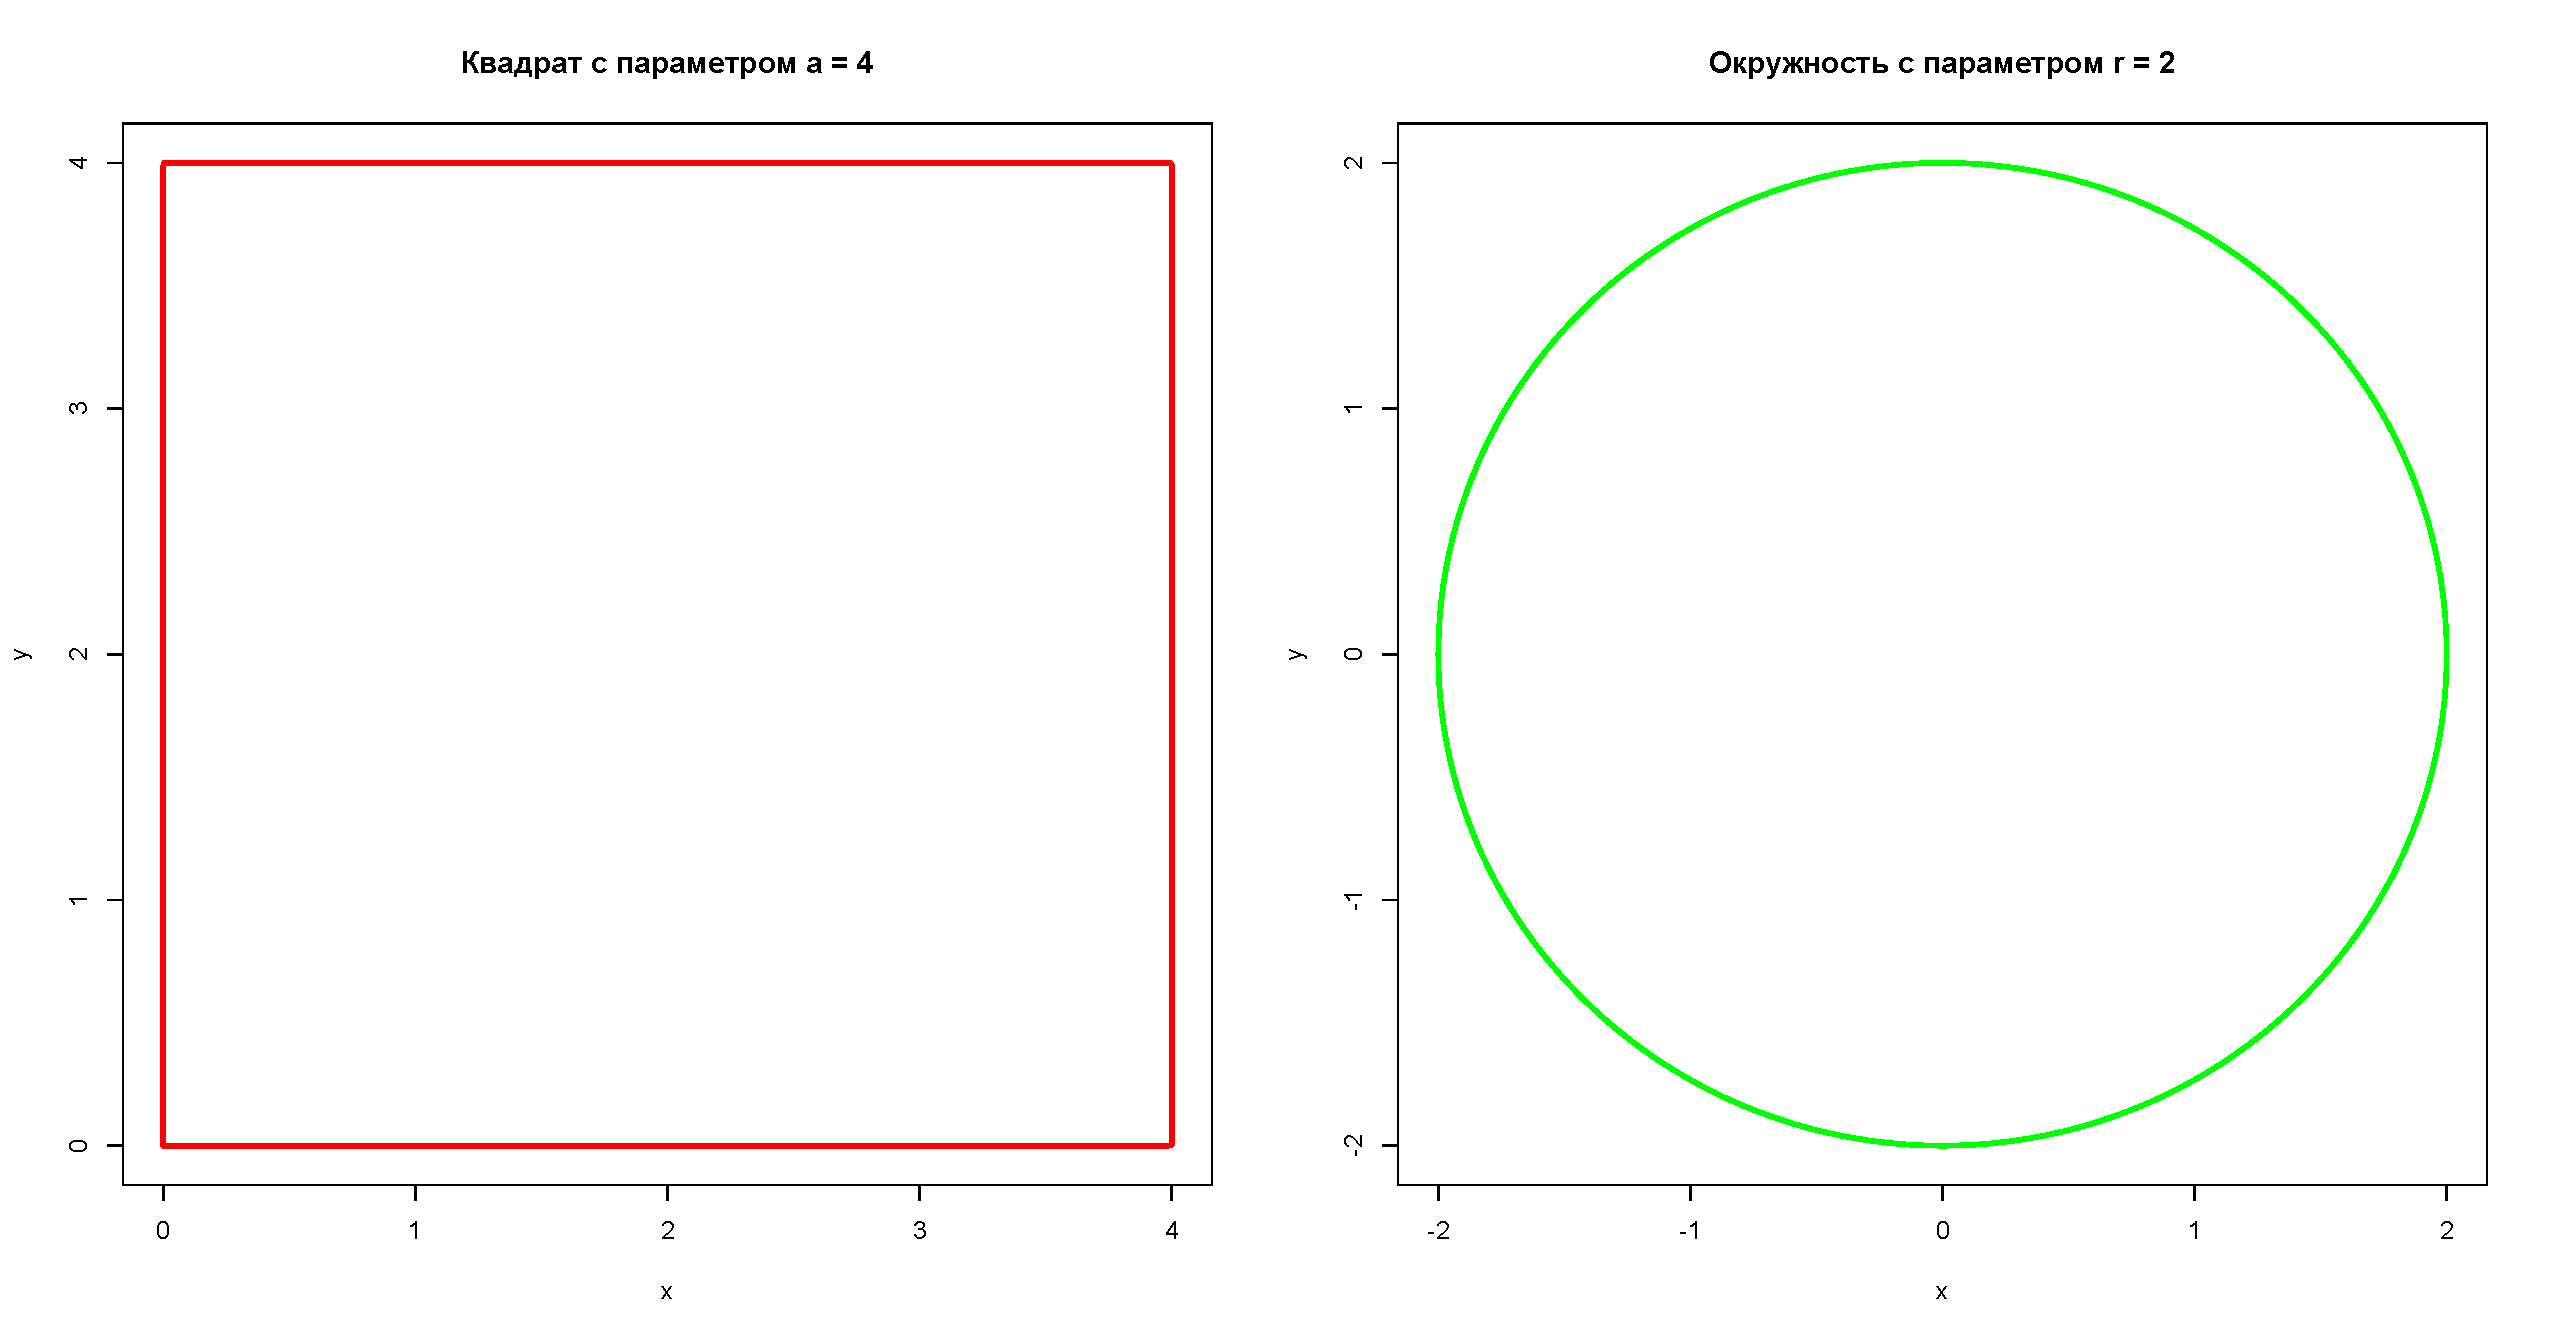
\includegraphics[width=\linewidth]{01.pdf}
  }
    \caption{Квадрат при $a=4$ и окружность при $r=2$}
    \label{kvci}
    \end{figure} 

    \item Аналогично равносторонний треугольник со стороной $a$, расположенный в первом квадранте, имеющий сторону, параллельную $oX$, и вершину в начале координат, имеет границу:
    \[
        x(t,a) =
        \begin{cases}
        t, & \text{если $t \in [0,a]$;} \\
        3a-2t, & \text{если $t \in [a,1\frac{1}{2}a]$.} \\
        \end{cases},
        y(t,a) =
        \begin{cases}
        t \sqrt{3}, & \text{если $t \in [0,\frac{1}{2}a]$;} \\
        -t \sqrt{3}+a\sqrt{3}, & \text{если $t \in [\frac{1}{2}a,a]$;} \\
        0, & \text{если $t \in [a,1\frac{1}{2}a]$.} \\
        \end{cases}
        \]
        Такой треугольник при $a=2$ изображён на Рис. \ref{tros}.

    \item Область, чья граница есть $S_1 \bigcup S_2 \bigcup S_3$, где $S_1=\{(x,y): y=0, x \in [0, a]\},S_2=\{(x,y): y=\sqrt{a^2-x^2}, x \in [\frac{1}{2}a, a]\},S_3=\{(x,y): y=\sqrt{a^2-(x-a)^2}, x \in [0,\frac{1}{2} a]\}$, может определяться через функции:       
    \[
        x(t,a) =
        \begin{cases}
        t, & \text{если $t \in [0,a]$;} \\
        2a-t, & \text{если $t \in [a,2a]$.} \\
        \end{cases},
        y(t,a) =
        \begin{cases}
        \sqrt{a^2-(t-a)^2}, & \text{если $t \in [0,\frac{1}{2}a]$;} \\
        \sqrt{a^2-t^2}, & \text{если $t \in [\frac{1}{2}a,a]$;} \\
        0, & \text{если $t \in [a,2a]$.} \\
        \end{cases}
        \]
        Такую область будем называть "острием". "Острие" при $a=2$ изображёно на Рис. \ref{tros}.
        
        \begin{figure}[h!]
          \noindent\centering{
          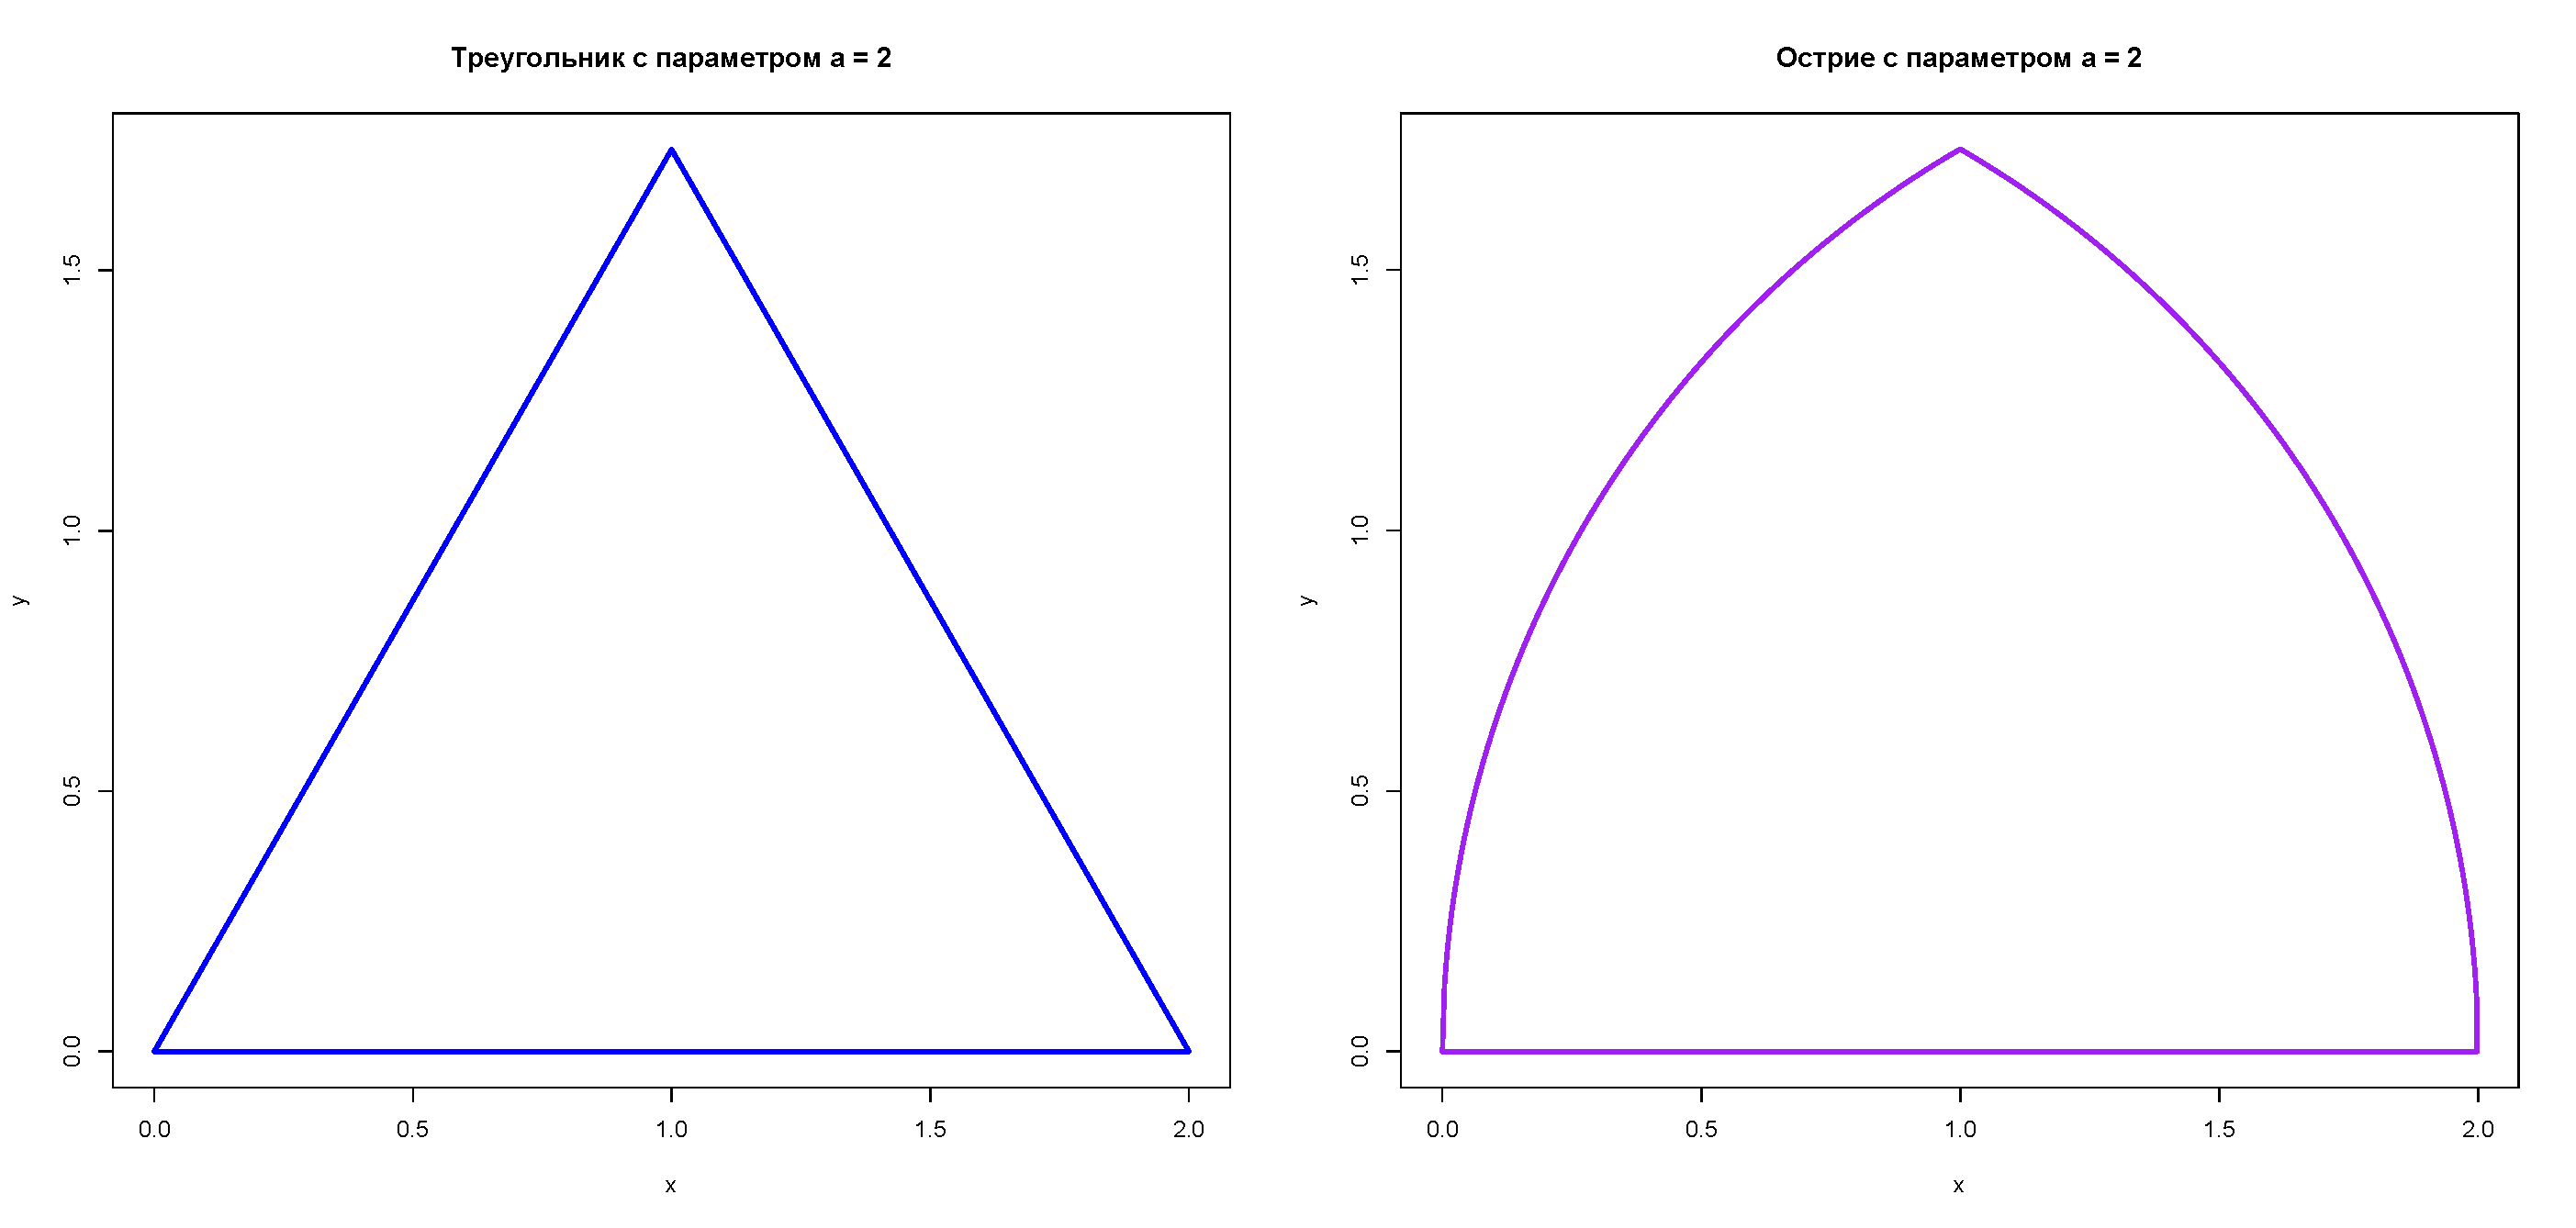
\includegraphics[width=\linewidth]{02.pdf}
        }
          \caption{Треугольник и "острие" при $a=2$}
          \label{tros}
          \end{figure}  
\end{enumerate}

Точно таким же образом особенно удобно задавать области, границы которых суть кусочно-гладкие кривые вида $S_i=\{(x,y): y=f_i(x), x \in [x_{i_0};x_{i_{\max}}]\}, i=1,2,\dots, n$, причём на каждом куске не имеет значения, задаётся ли кривая в декартовой системе координат или в полярной.

{\bf Замечания}: 

\begin{enumerate}
  \item В указанных примерах используется простейшая параметризация, но её недостаток в том, что во всех примерах, кроме первого, при изменении радиуса $r$ кривой меняется и расположение её центра, из-за чего при разных параметрах $r_1,r_2$ кривые ${\bf r}(t,r_1),{\bf r}(t,r_2)$ имеют общие точки, что не подходит для алгоритма.
Проблема исправляется фиксацией центра в некоторой точке и заданием кривых относительно этого центра. Например, квадрат с центром в $(x_0;y_0)$ и длиной стороны $a$ имеет параметризацию:
\[
x(t,a) =
\begin{cases}
x_0-\frac{1}{2}a+t, & \text{если $t \in [0,a]$;} \\
x_0+\frac{1}{2}a, & \text{если $t \in [a,2a]$;} \\
x_0+\frac{1}{2}a-(t-2a), & \text{если $t \in [2a,3a]$;} \\
x_0-\frac{1}{2}a, & \text{если $t \in [3a,4a]$.} \\
\end{cases},
y(t,a) =
\begin{cases}
y_0-\frac{1}{2}a, & \text{если $t \in [0,a]$;} \\
y_0-\frac{1}{2}a+(t-a), & \text{если $t \in [a,2a]$;} \\
y_0+\frac{1}{2}a, & \text{если $t \in [2a,3a]$;} \\
y_0+\frac{1}{2}a-(t-3a), & \text{если $t \in [3a,4a]$.} \\
\end{cases}.
\]
Теперь, меняя значение параметра $a$, мы получаем вложенные друг в друга квадраты с общим центром (Рис. \ref{rects}).
\begin{figure}[h!]
  \noindent\centering{
  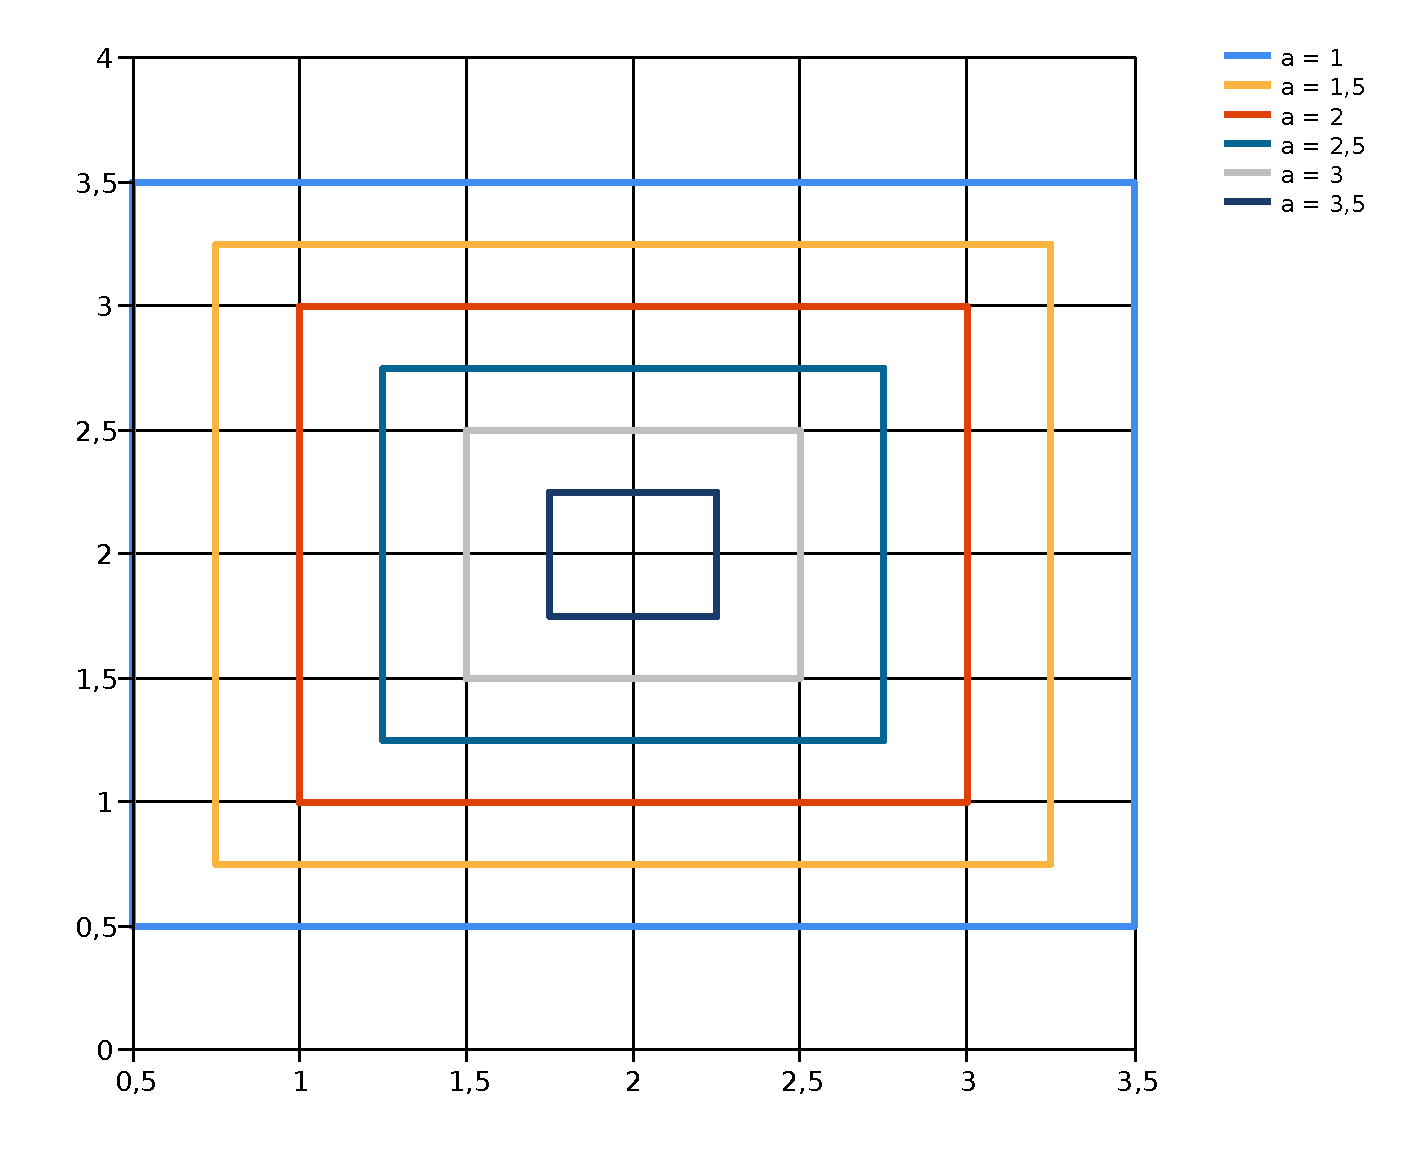
\includegraphics[width=0.8\linewidth]{rect.pdf}
}
  \caption{Вложенные квадраты с центром $(2;2)$}
  \label{rects}
  \end{figure}
  
  \item Если кривая уже задана параметрическими функциями $x=x(t),y=y(t)$, чаще всего (кроме случаев, когда она проходит через некоторый центр, относительно которого задана \footnote{К примеру, для окружности естественным будет её геометрический центр, но есть взять замкнутую полуокружность (концы соединены друг с другом отрезком), то естественным будет задать эту полуокружность относительно центра окружности, но в этом случае она будет проходить через центр, поэтому такая параметризация не может использоваться, т. к. с уменьшением радиуса происходит сжатие не во внутрь фигуры. В Приложении А имеется пример составления параметризации для полукруга.}) подобные вложенные кривые можно получить домножением $x,y$ на радиус $r$.
  В этом случае даже не очевидно, что именно является "центром"\ кривой, но этот центр легко сдвигать прибавлением к $x,y$ координат вектора переноса.
  На рисунках \ref{r1}-\ref{r2} это правило используется для базовой кривой, заданной формулами
\[
\begin{cases}
  x(t)=(R-r)\cos\left(\frac{r}{R}t\right)+h \cos \left(t-\frac{r}{R}t\right),\\
  y(t)=(R-r)\sin\left(\frac{r}{R}t\right)-h \sin \left(t-\frac{r}{R}t\right),\\
  r=\dfrac{1}{3}, h=\dfrac{1}{4}
\end{cases}.  
\]

  \begin{figure}[h]
    \begin{center}
    \begin{minipage}[h]{0.49\linewidth}
    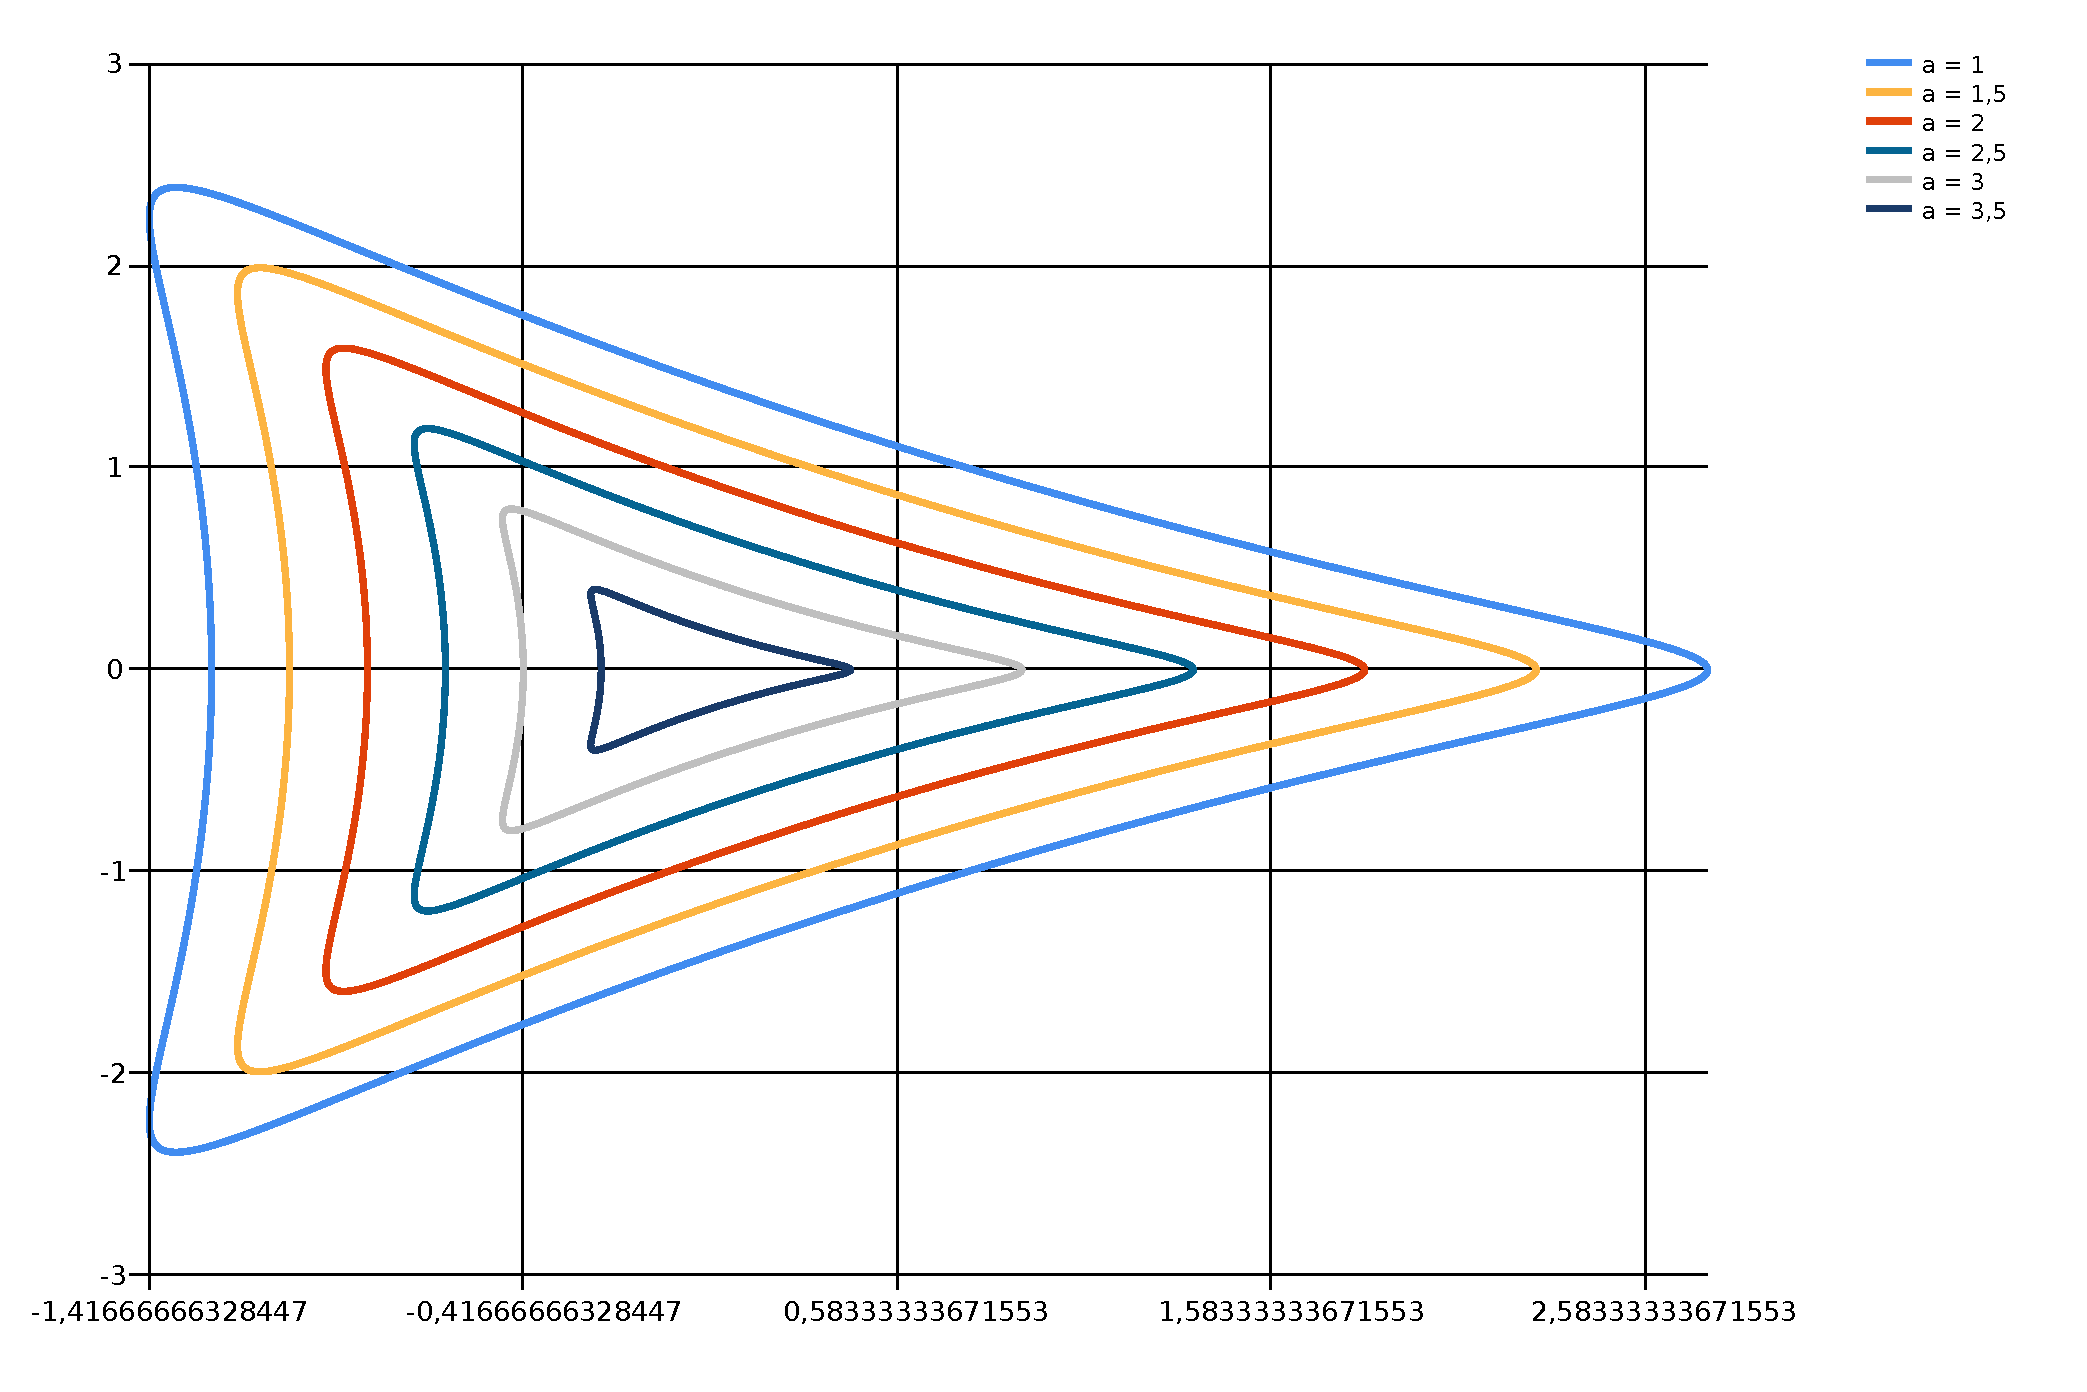
\includegraphics[width=1\linewidth]{r1.pdf}
    \caption{$R=1$} %% подпись к рисунку
    \label{r1} %% метка рисунка для ссылки на него
    \end{minipage}
    \hfill 
    \begin{minipage}[h]{0.49\linewidth}
    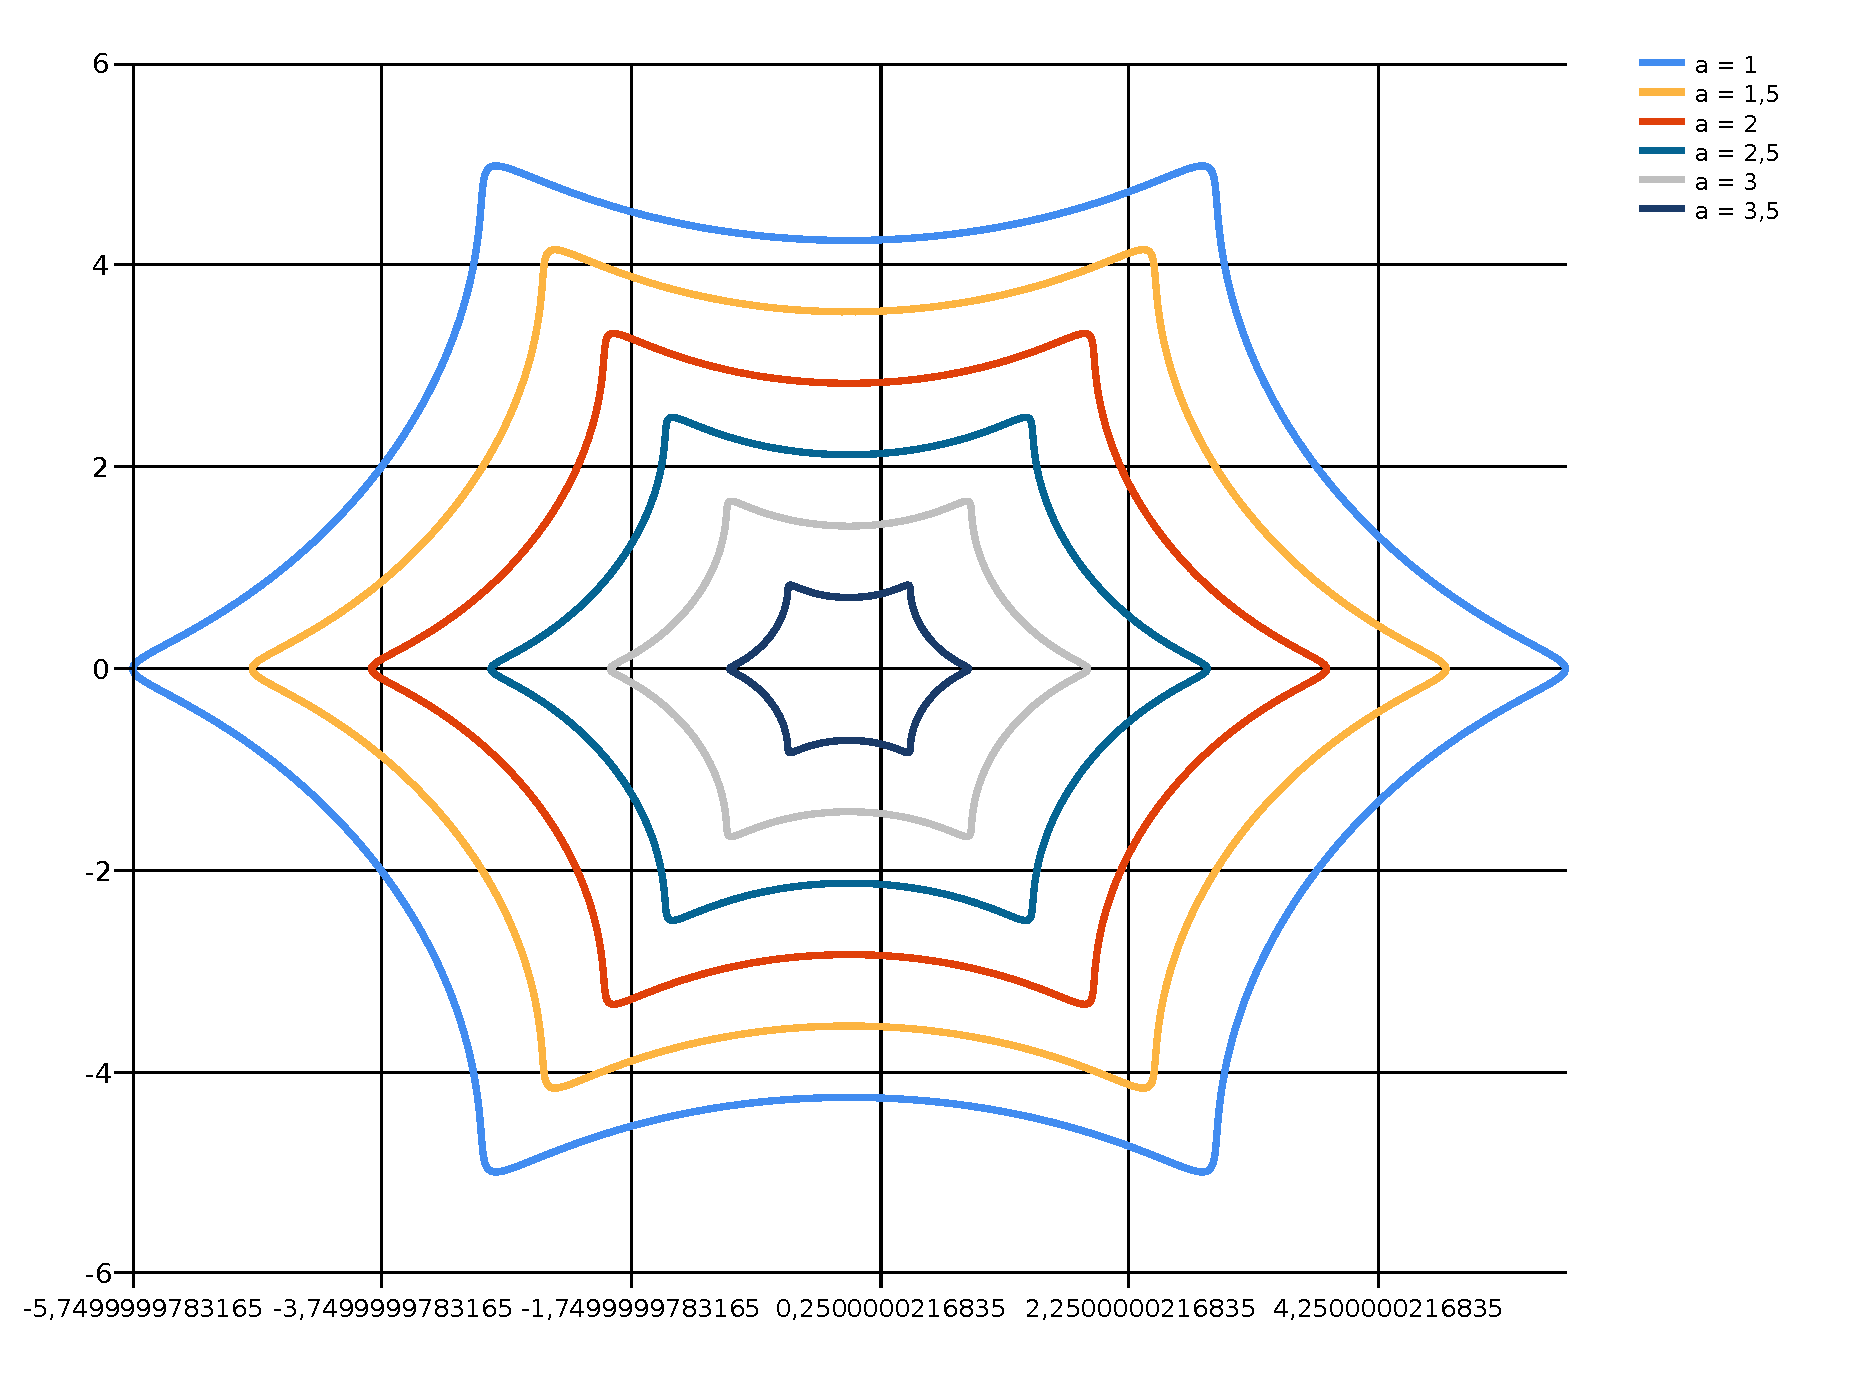
\includegraphics[width=1\linewidth]{r2.pdf}
    \caption{$R=2$}
    \label{r2}
    \end{minipage}
    \end{center}
    \end{figure}
\end{enumerate}


\subsection{Описание алгоритма}
Расположим в открытом множестве $Q^+= \R{n}\backslash \bar Q$ точки $z_1,z_2,\dots,z_N$ (базисные точки). От положения этих точек будет зависеть точность решения, однако пока неизвестно, какое именно положение точек будет оптимальным.
Известно, что во многих случаях существуют наборы точек, дающие наилучшее решение задачи вплоть до машинного нуля, как есть и крайне неоптимальные наборы точек, которые не будут давать точного решения даже в тривиальном случае.
Во всяком случае, точки требуется располагать по какому-то правилу, чтобы результаты экспериментов можно было сравнивать.
Пока будем располагать точки равномерно возле подобной $S$ поверхности большего радиуса, при этом сами точки должны располагаться с небольшими случайными отклонениями в ту или другую сторону по нормали от $S$.

\begin{figure}[!h]
    \noindent\centering{
    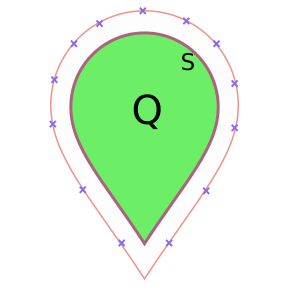
\includegraphics[width=120mm]{il1}
    }
    \caption{Образец расстановки базисных точек в $\R{2}$}
\end{figure}


Расставив точки, будем искать приближённое решение ОЗГ $\tilde \rho_N$ в виде
\begin{equation}
    \tilde \rho_N=\sum_{i=1}^N c_i \alpha_i,
\end{equation}
где $\alpha_i=\alpha_i(z)=E(z-z_i),c_i \in \mathbb{R}$ определяются из решения задачи минимизации функционала
\begin{equation}
    F(c)=F(c_1,\dots,c_N)=\Bigr|\Bigr|V_{\sum_{i=1}^N c_i \alpha_i} -\varphi\Bigr|\Bigr|_{L_2(S)} \rightarrow \min, \varphi =V_{\rho} \equiv \V{\rho}. 
\end{equation}

Нетрудно показать, что $F$ --- квадратичный функционал, а задача его минимизации эквивалентна решению системы линейных алгебраических уравнений
\begin{equation}
    \begin{pmatrix}
        (\omega_1, \omega_1) & (\omega_1, \omega_2) & \cdots & (\omega_1, \omega_N)\\
        (\omega_2, \omega_1) & (\omega_2, \omega_2) & \cdots & (\omega_2, \omega_N)\\
        \hdotsfor{4}\\
        (\omega_N, \omega_1) & (\omega_N, \omega_2) & \cdots & (\omega_N, \omega_N)\\
    \end{pmatrix}
    \begin{pmatrix}
        c_1\\
        c_2\\
        \cdots\\
        c_N\\
    \end{pmatrix}
    =
    \begin{pmatrix}
        (\omega_1,\varphi)\\
        (\omega_2,\varphi)\\
        \cdots\\
        (\omega_N,\varphi)\\
    \end{pmatrix},
    \label{gram}
\end{equation}
где 
\begin{equation}
    \omega_i(x)=\V{\alpha_i}
\end{equation}
и скобки $(\cdot,\cdot)$ обозначают скалярное произведение:
\begin{equation}
    (f,g)=(f,g)_{L_2(S)}=\int_S f(x)g(x) ds.
\end{equation}

Заметим, что мы свели решение ОЗГ к решению задачи аппроксимации функции $\varphi$ системой функций $\omega_i$. 

\subsection{Детали реализации}
\subsubsection{Кратное интегрирование}
Для интегрируемой функции $f$ и области $Q$ на прямоугольной области $D \supseteq Q$ определим функцию
\begin{equation*}
  g(x)=
  \begin{cases}
    f(x), & x \in Q\\
    0, & x \not \in Q
  \end{cases}.
\end{equation*}
Интеграл от функции $f$ считается как интеграл от функции $g$ методами библиотеки Math.NET Numerics (\url{https://numerics.mathdotnet.com})
по квадратурам Гаусса-Лежандра при числе узлов $n=128$.

До этого автором использовались лично написанные методы интегрирования, которые  не удовлетворяли либо в точности, либо по производительности, поэтому было решено использовать сторонние методы.

\subsubsection{Устойчивое решение СЛАУ, связанной с задачей аппроксимации}

Известно, что матрица системы (\ref{gram}) --- это матрица Грама, а численное решение такой системы составляет отдельную задачу, поскольку классические методы решения и их простые комбинации дают неустойчивое решение.
Наибольший вклад в неустойчивость аппроксимации вносят три причины:

\begin{enumerate}
\item  Скалярные произведения, заполняющие СЛАУ, обычно представляются конечными суммами или интегралами; при этом это могут быть интегралы по сложным областям или поверхностям или интегралы от функций, которые сами задаются интегралами; в таком случае погрешности квадратурных формул накапливаются и приводят к тому, что исходная СЛАУ несколько отличается от истинной, что негативно сказывается на решении задачи. Даже если удаётся подобрать реализуемый способ интегрирования, часто попытки повысить точность существенно увеличивают время вычислений.

\item  Матрица Грамма для любой системы функций является плохо обусловленной по определению, причём число обусловленности быстро растёт с увеличением размерности, из-за чего даже малые отклонения в элементах системы (которые будут иметь место хотя бы по причине пункта 1) приводят к неточным решениям.

\item  Огромную роль играют погрешности округления при суммировании больших и маленьких чисел, делении и умножении; эти погрешности заметны при вычислении интегралов, решении СЛАУ и даже при замене координат (для получения системы, ортогональной на произвольном отрезке).
При плохо обусловленной матрице системы даже итерационные методы не способны из-за ошибок округления приблизиться к истинному решению ближе некоторого расстояния. Комбинация пунктов 1) и 3) приводит к тому, что даже аппроксимация по  ортогональным системам обладает неустойчивостью при достаточно большом числе функций.
\end{enumerate}

Имеется алгоритм решения таких систем, дающий устойчивое решение, который и будет использован.
Назовём его {\it ультра-гибридным} .
Он заключается в следующем. Допустим, требуется минимизировать функционал вида
\begin{equation}
  F\left(c^M\right)={\left\|\varphi -\sum^M_{m=1}{c_m}{\alpha }_m\right\|}_{{\ L}_2\left(\partial Q\right)},\ c^M=(c_1,\dots,c_M), \varphi, \alpha_m \text{известны},
\end{equation} 
причём его минимизация должна удовлетворять условию
\begin{equation}F\left(c^{M-1}\right)\ge F\left(c^M\right)\ge F\left(c^{M+1}\right),\ M\ge 2.
\end{equation} 
Такую минимизацию можно осуществить по индукции:

Если $M=1$, решение очевидно: $c_1=\left({\alpha }_1,\varphi \right)/\left({\alpha }_1,{\alpha }_1\right)$. В противном случае требуется искать решения для $c^2$, $c^3$,{\dots}, $c^{M-1}$ последовательно; допустим, они найдены, тогда:

Шаг 1 (СПИДГАУСС)\footnote{ Специфические названия шагов метода связаны с историей его создания: ультра-гибрид является комбинацией методов Гаусса, наискорейшего спуска и покоординатной минимизации с акцентом на последний. Включение других методов решения СЛАУ либо уточнения решения не дало результатов в том числе потому, что, оказывается, матрица Грама не является положительно определённой в численном плане, поэтому при решении такой СЛАУ методом Холецкого и пр., рассчитанными на положительно определённые матрицы, возникают корни из отрицательных чисел, т. е. NaN, а итерационные методы расходятся; есть предположение, что это явление связано с погрешностями при вычислении сумм чисел разного порядка.}.
Найти вектор $c^M=\left(c_1,c_2,\dots ,c_M\right)$, решив известную СЛАУ каким-либо классическим методом (в том числе методом Гаусса или методом Гаусса с уточнением решения методом наискорейшего спуска и т. п.).

Шаг 2 (МИНИМАКА СПИДГАУССА). Если $F\left(c^{M-1}\right)<F\left(c^M\right)$, то применить ко всем компонентам $c^M$ покоординатную минимизацию (возможно, несколько раз) по формуле
\begin{equation}
  c_k=\frac{\left({\alpha }_k,\varphi \right)-\sum^N_{m=1,m\neq k}{c_m}\left({\alpha }_k,{\alpha }_m\right)}{\left({\alpha }_k,{\alpha }_k\right)}.
\end{equation}

Шаг 3 (ПОЛНАЯ МИНИМАКА). Если снова $F\left(c^{M-1}\right)<F\left(c^M\right)$, то вектор $c^M$ заменить на вектор $\left(c^{M-1}_1,c^{M-1}_2,\dots ,c^{M-1}_{M-1},0\right)$ и провести покоординатную минимизацию по всем компонентам этого вектора.

Шаг 4 (МИНИМАКА НА КОНЦЕ). Если снова $F\left(c^{M-1}\right)<F\left(c^M\right)$, то вектор $c^M$ снова заменить на вектор $\left(c^{M-1}_1,c^{M-1}_2,\dots ,c^{M-1}_{M-1},0\right)$ и применить покоординатную минимизацию только для последнего элемента
\begin{equation}c^M=\left(c^{M-1}_1,c^{M-1}_2,\dots ,c^{M-1}_{M-1},\frac{\left({\alpha }_M,\varphi \right)-\sum^{M-1}_{m=1}{c_m}\left({\alpha }_M,{\alpha }_m\right)}{\left({\alpha }_M,{\alpha }_M\right)}\right).\end{equation} 

Шаг 5. Если и в таком случае $F\left(c^{M-1}\right)<F\left(c^M\right)$, то 
\begin{equation}c^M=\left(c^{M-1}_1,c^{M-1}_2,\dots ,c^{M-1}_{M-1},0\right)\to F\left(c^{M-1}\right)=F\left(c^M\right).\end{equation} 

Практика показывает, что шаги 1-4 не являются равнозначными и в каждом конкретном случае любой из них может уменьшить погрешность аппроксимации там, где остальные не могут.
Во многих случаях на каждом шаге точность аппроксимации увеличивается хотя бы на доли процента.

В следующей таблице показан пример поведения ультра-гибрида, полученный из реального решения задачи ОЗГ на границе круга радиуса 0.5 при граничной функции $f(x,y)=x+y$.
Пусть на нулевом шаге метода все коэффициенты $c_i$ равны 0, тогда $||f-\sum_i c_i \alpha_i||=||f||$ --- начальная погрешность.
\begin{center}
\begin{tabular}[t]{|c|c|c|}
  \hline
  При размерности подсистемы & аппроксимация улучшилась на & на шаге метода \\
  \hline
  1 & 77,9387892163706 \% & СПИДГАУСС \\
  2 & 84,9337396999316\% & СПИДГАУСС\\
6& 0,0131813672596741\% &МИНИМАКА НА КОНЦЕ\\
7& 22,9523377376523\% &СПИДГАУСС\\
8& 2,68164131277237E-05\% &СПИДГАУСС \\
9& 1,66694595002183\% &СПИДГАУСС \\
10& 0,00010090869733369\% & ПОЛНАЯ МИНИМАКА\\
11& 1,96385711795082\% & СПИДГАУСС\\
14&  5,46330664269579E-05\% &МИНИМАКА НА КОНЦЕ\\
17& 0,00018143331403764\% & МИНИМАКА НА КОНЦЕ\\
18& 4,24842896257656E-05\% &МИНИМАКА НА КОНЦЕ\\
21& 8,51067538277787\% & ПОЛНАЯ МИНИМАКА \\
22& 1,12311108019212\% & МИНИМАКА СПИДГАУССА\\
32&  0,00370215728763344\% & МИНИМАКА НА КОНЦЕ\\
36& 11,4760683358568\% & МИНИМАКА НА КОНЦЕ \\
37& 10,0566903537115\% & МИНИМАКА НА КОНЦЕ\\
38& 7,80997025050057\% &МИНИМАКА НА КОНЦЕ \\
39& 15,6181909756738\% &МИНИМАКА НА КОНЦЕ\\
40& 0,0123664635283655\% &МИНИМАКА НА КОНЦЕ\\
41& 0,502578273639463\% &МИНИМАКА НА КОНЦЕ\\
42& 0,0823846153521963\% &МИНИМАКА НА КОНЦЕ\\
43& 0,118850502903311\% &МИНИМАКА НА КОНЦЕ\\
44& 50,2684017885662\% &СПИДГАУСС\\
45& 5,08710811927707\% &МИНИМАКА НА КОНЦЕ \\
  \hline
  \end{tabular}
\end{center}

Следующие графики (Рис. \ref{monex}-\ref{log}) показывают, насколько метод устойчив;
обратите внимание, что зачастую ультра-гибрид позволяет аппроксимировать не только устойчиво,
но и точнее любого другого метода (в графиках о точности аппроксимации кривая ультра-гибрида опускается ниже минимального значения для другого метода).
На приведённых графиках разные функции аппроксимировались несколькими системами (при разной размерности систем):
\begin{itemize}
  \item Мономами: $1, x, x^2,\dots , x^k$
  \item Экспонентами: $1, e^x, e^{2x},\dots$
  \item Дробями: $1,\dfrac{1}{1+x^2}, \dots , \dfrac{1}{1+kx^2}$
  \item Логарифмами: $\ln\left(0.01 + \left(x+1-\dfrac{k}{10}\right)^2\right)$
\end{itemize}
Под неоптимизированной функцией (классическим решением) подразумевается результат аппроксимации, полученный при решении СЛАУ типа \ref{gram} методом Гаусса, другой вариант --- ультрагибридным методом.

\begin{figure}[h!]
  \noindent\centering{
  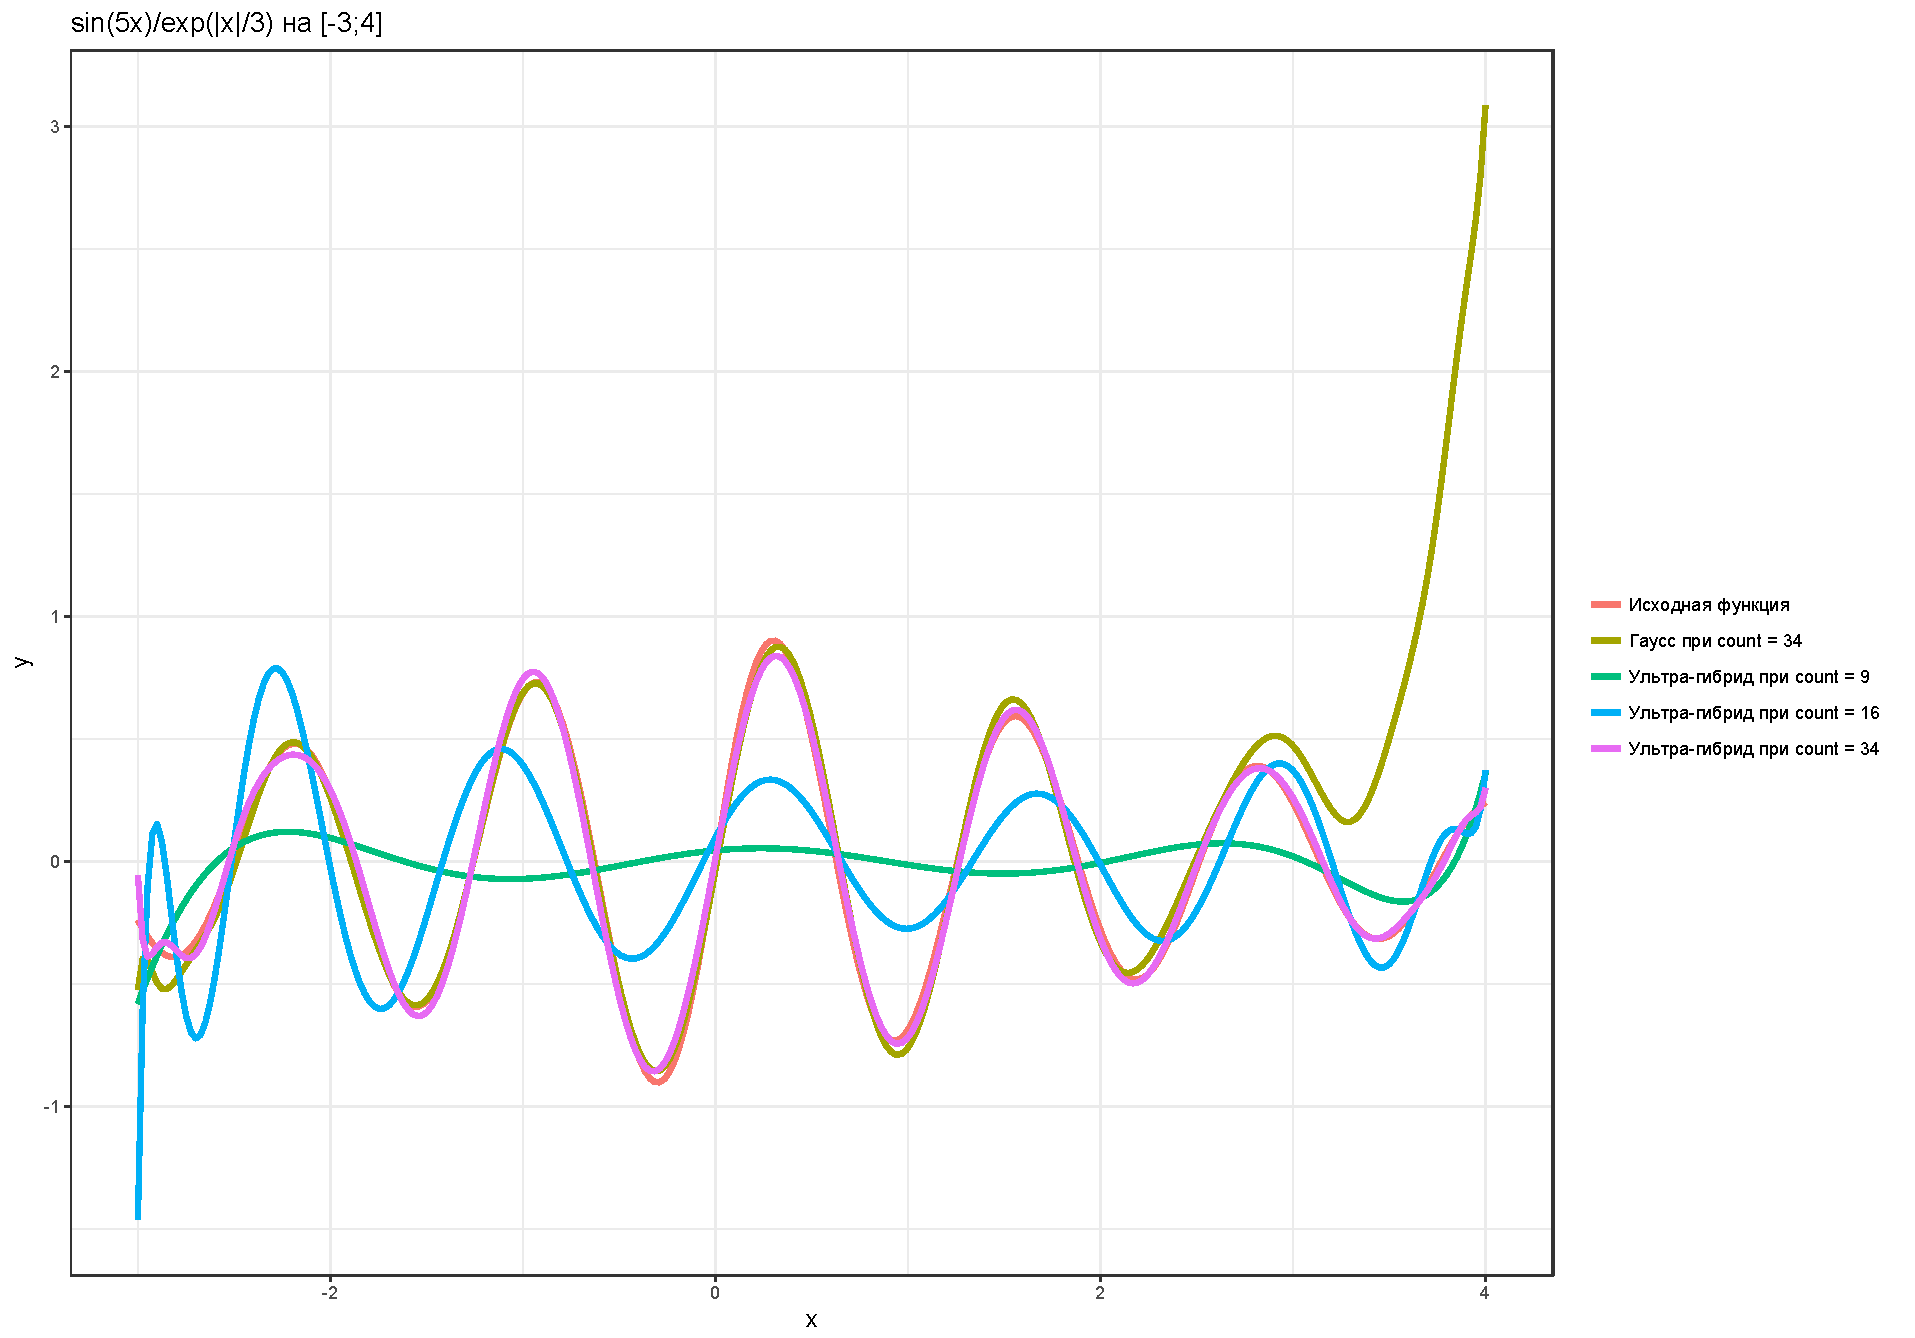
\includegraphics[width=\linewidth]{monex.pdf}
}
 \caption{Аппроксимация мономами}
  \label{monex}
\end{figure}

\begin{figure}[h!]
  \noindent\centering{
  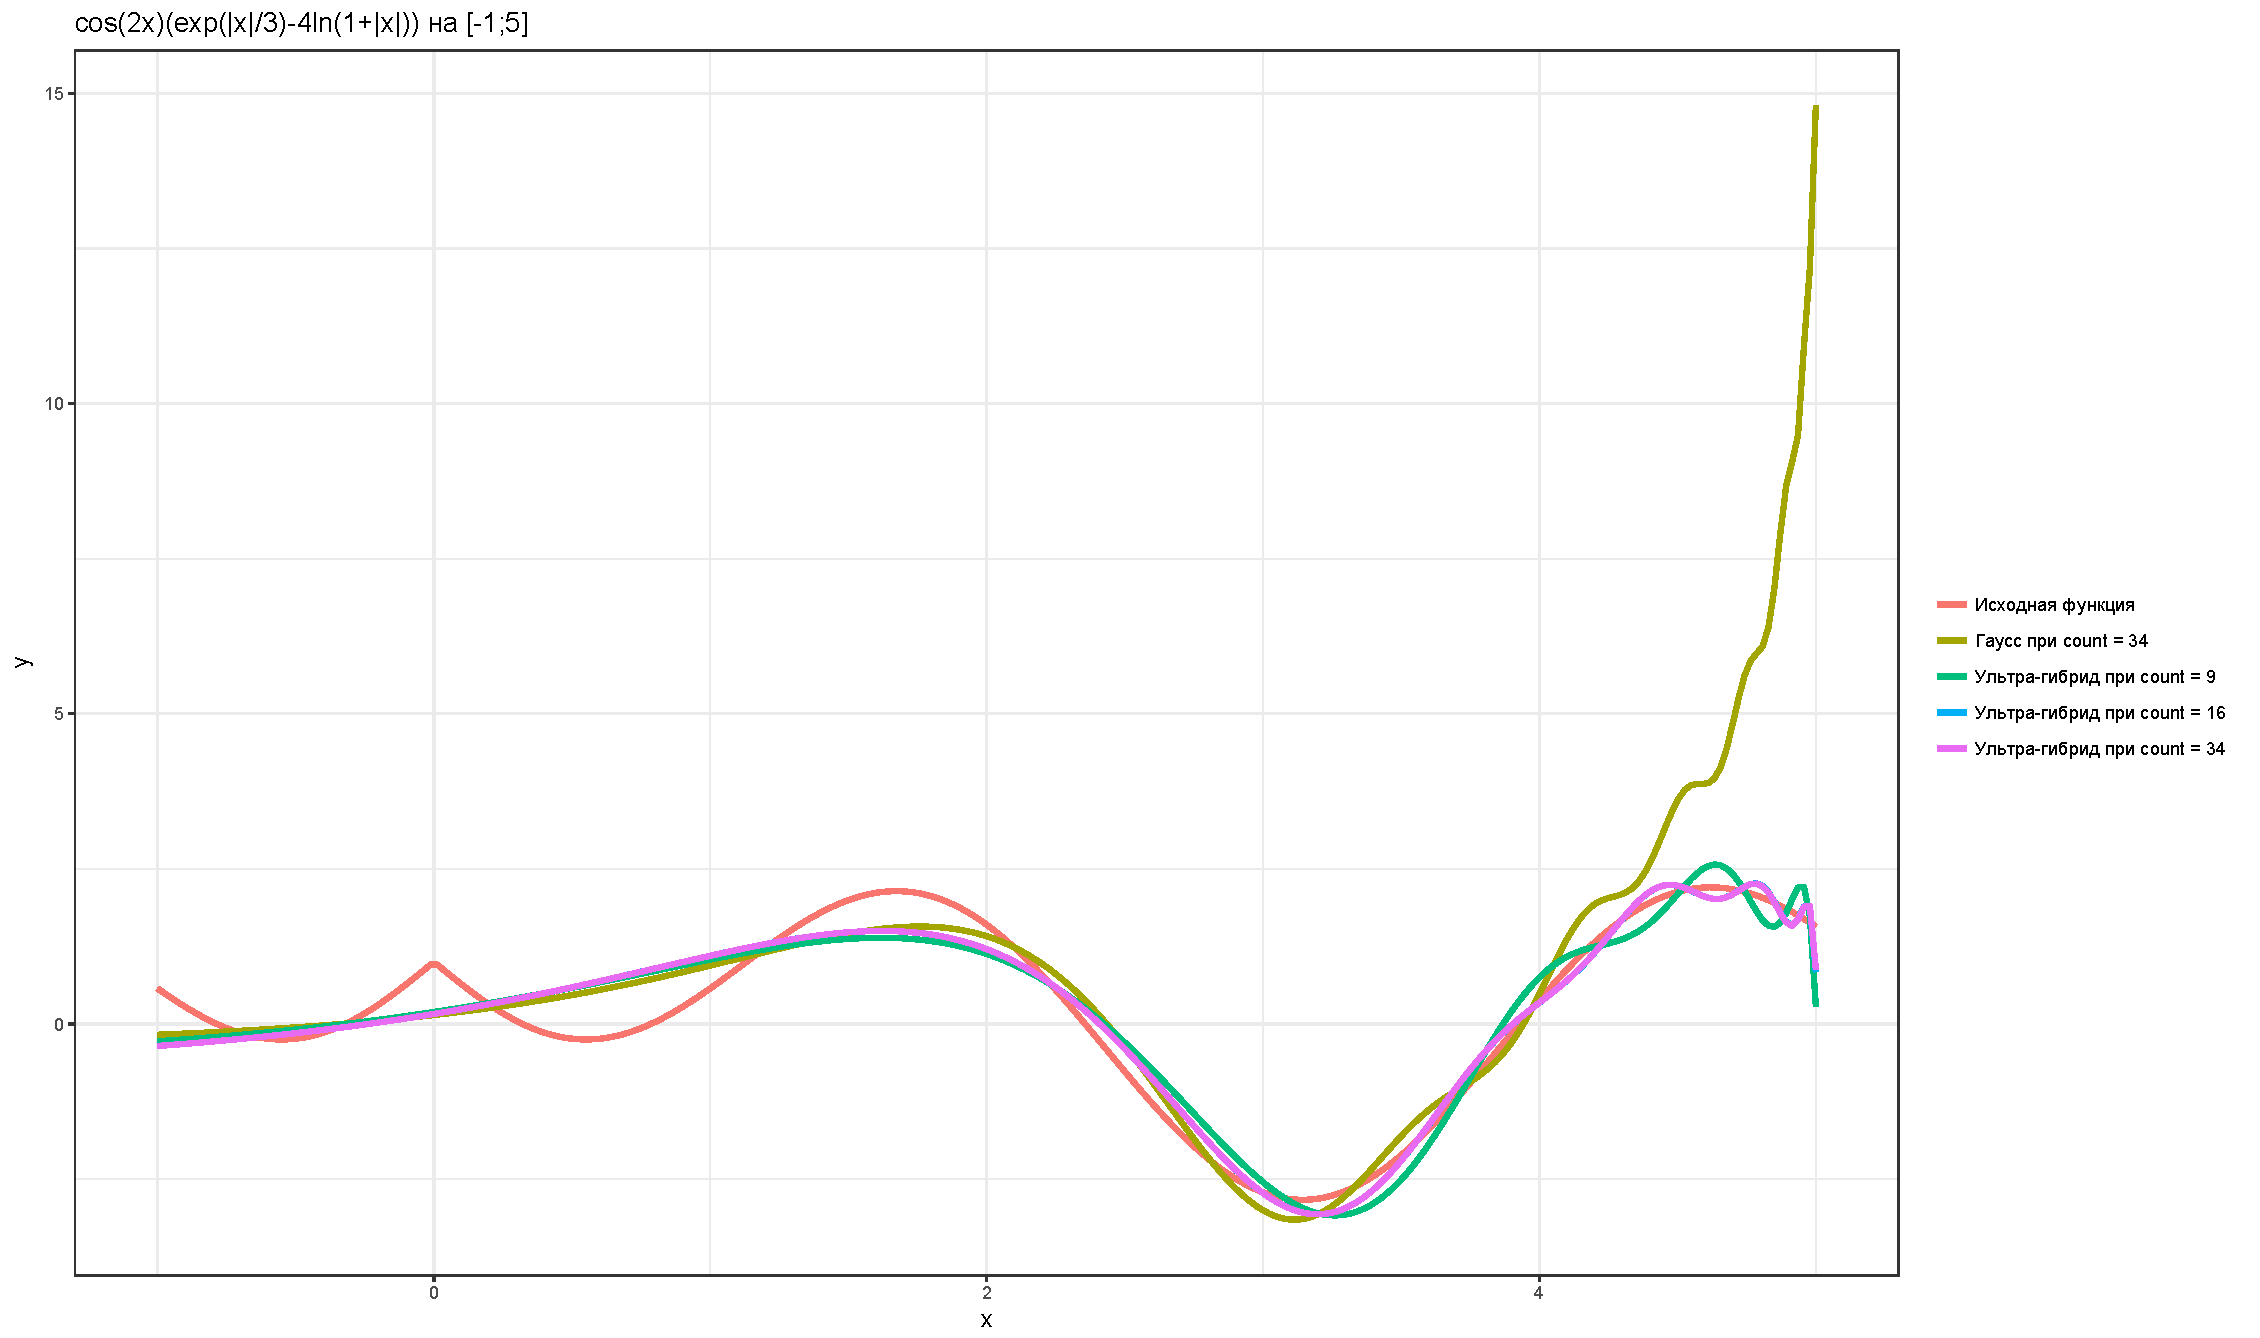
\includegraphics[width=\linewidth]{expex.pdf}
}
 \caption{Аппроксимация экспонентами}
  \label{expex}
\end{figure}

\begin{figure}[h!]
    \noindent\centering{
    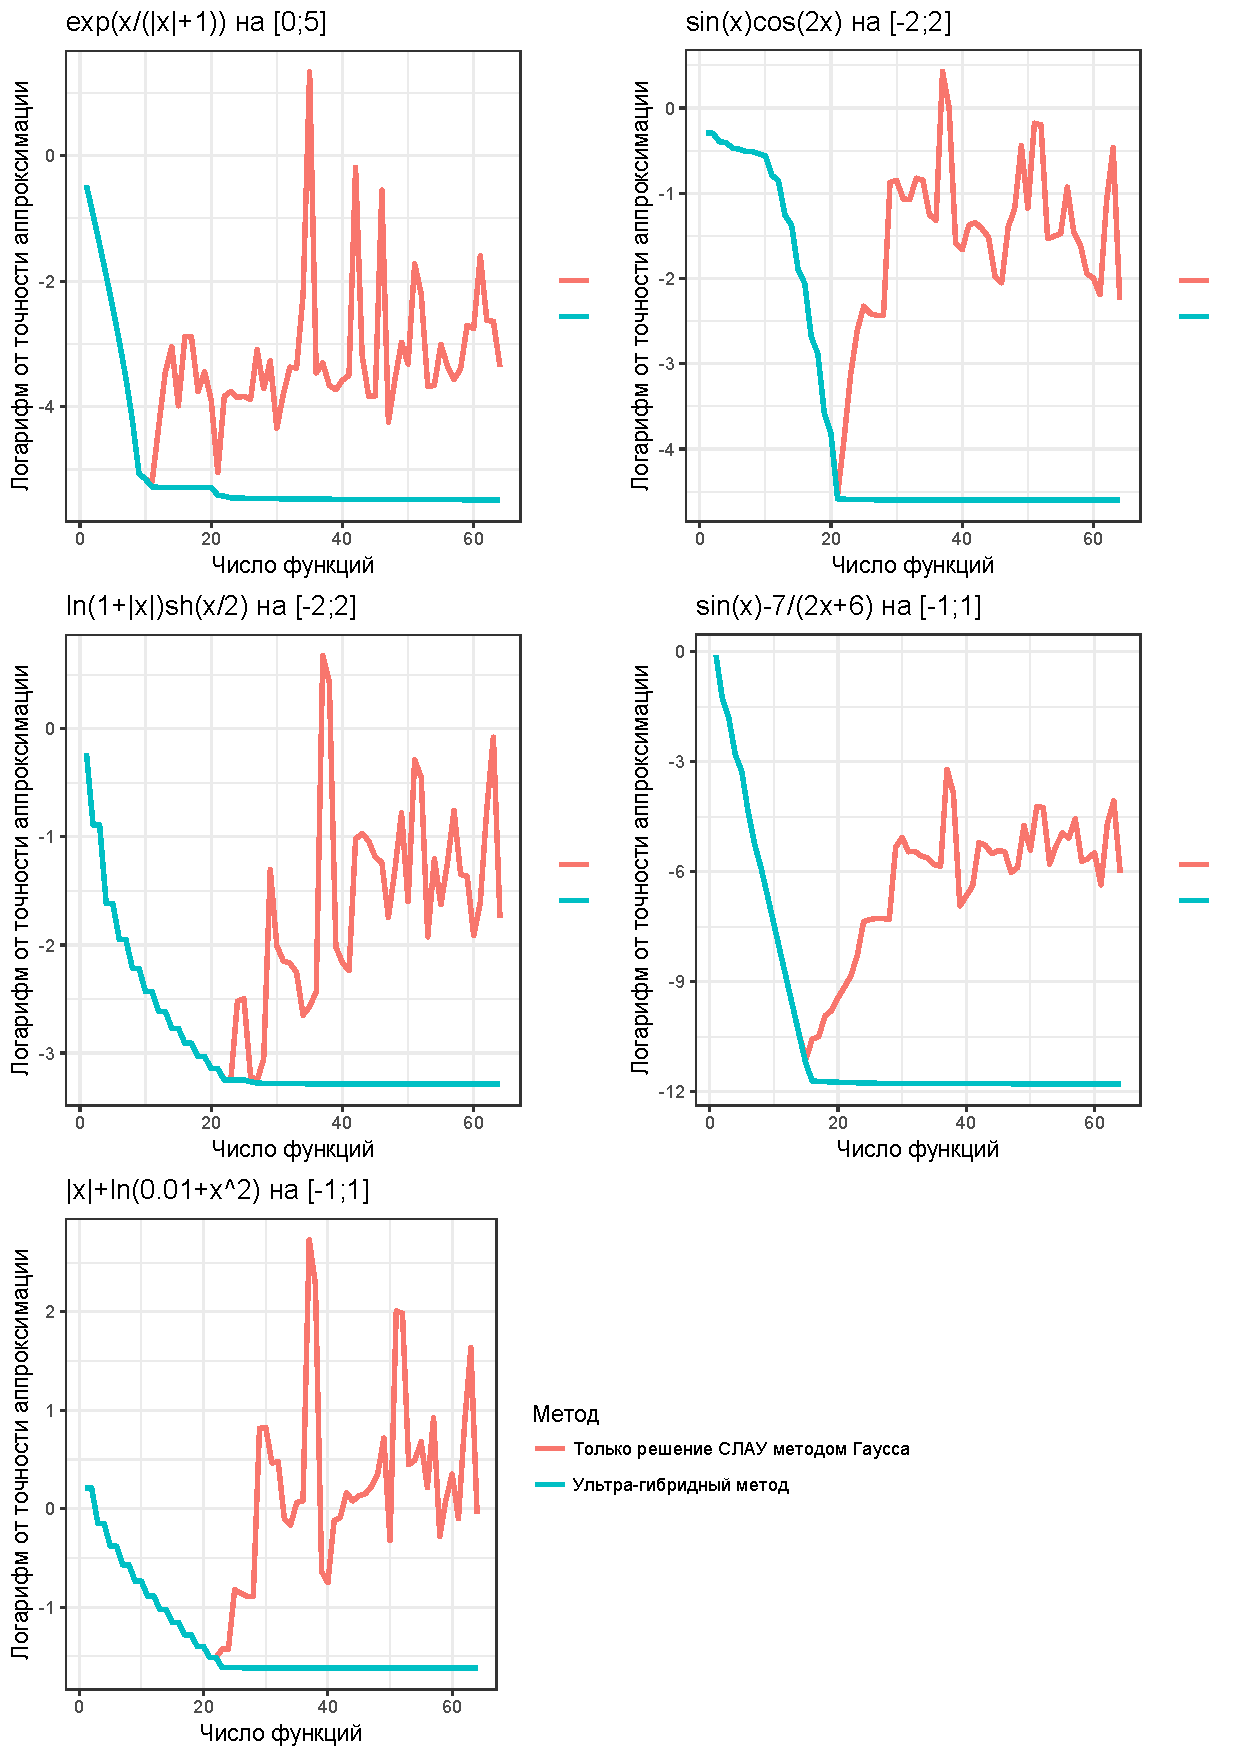
\includegraphics[width=0.9\linewidth]{mon.pdf}
  }
   \caption{Аппроксимация мономами}
    \label{mon}
\end{figure} 

\begin{figure}[h!]
    \noindent\centering{
    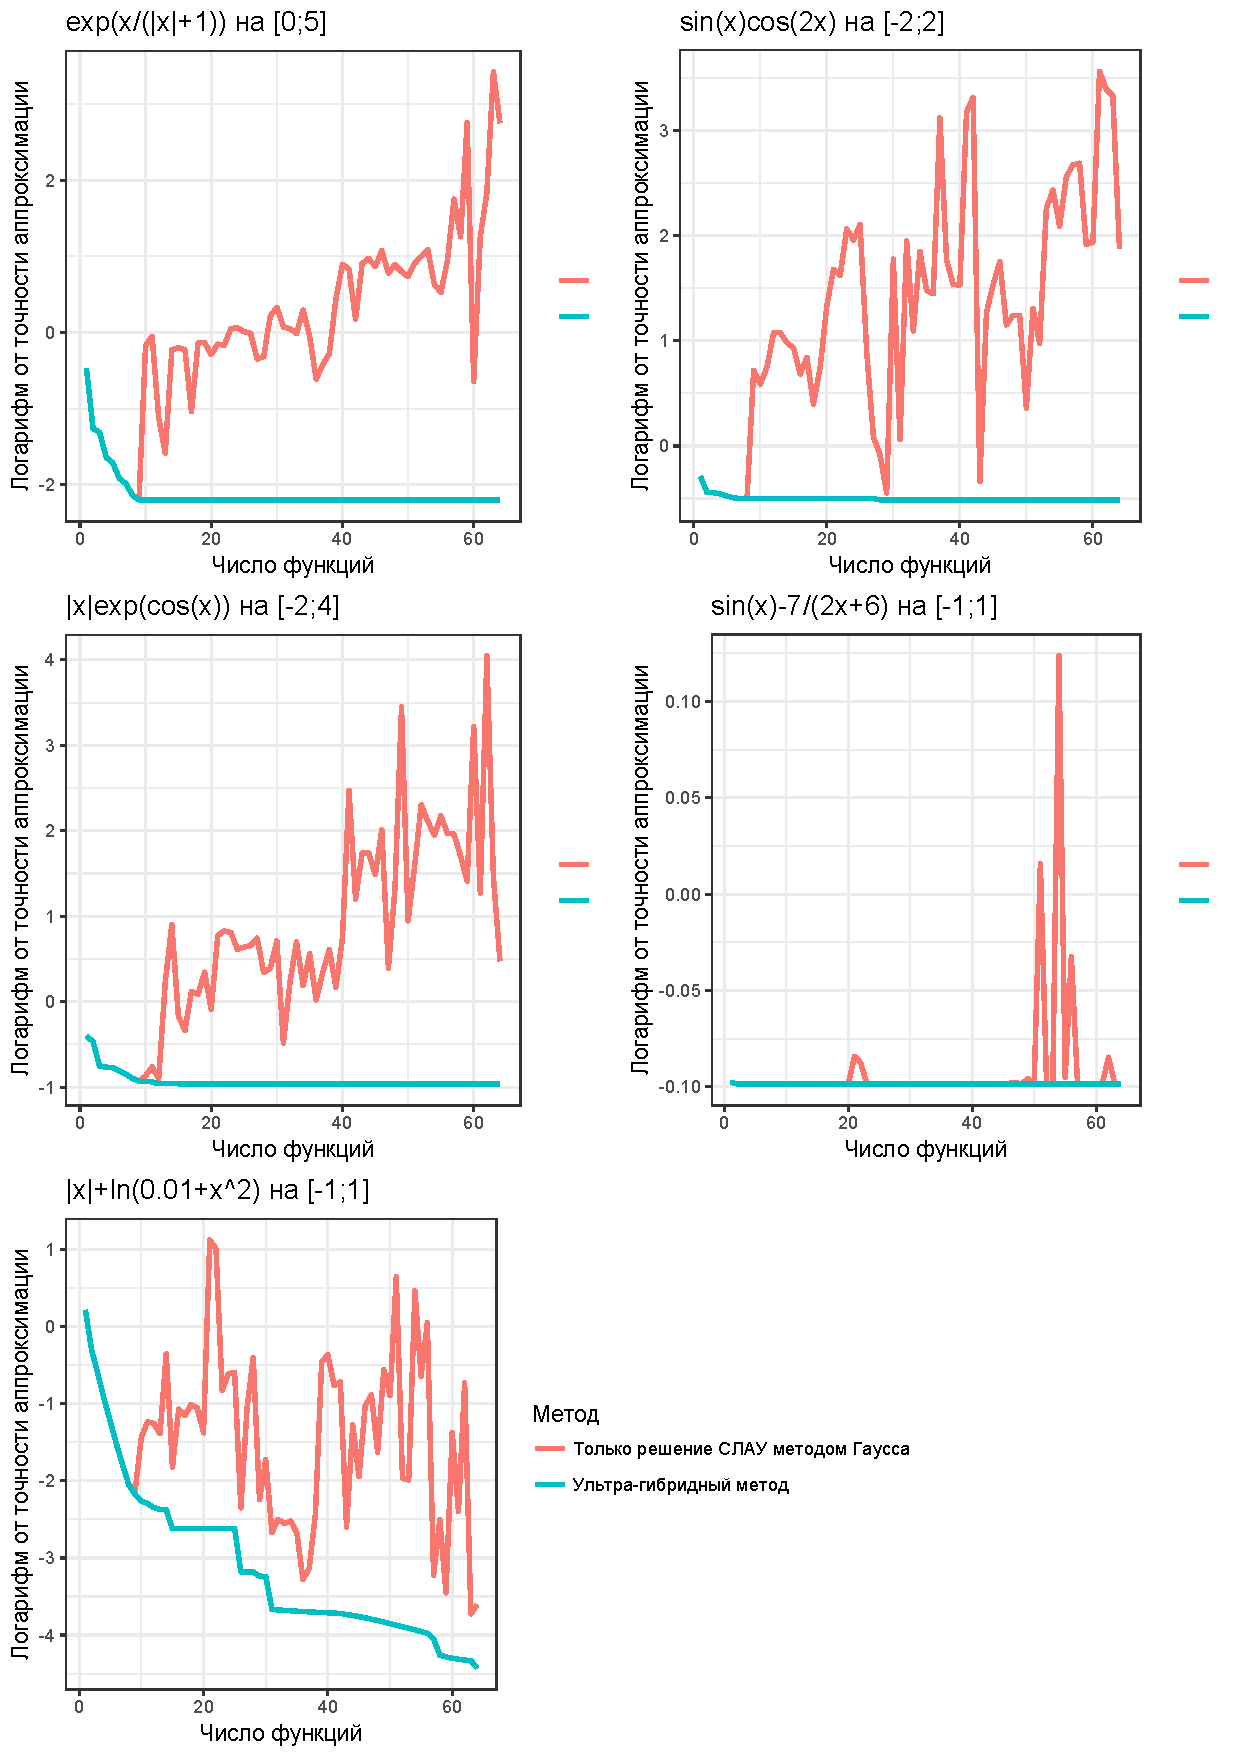
\includegraphics[width=0.9\linewidth]{rat.pdf}
  }
   \caption{Аппроксимация дробями}
    \label{rat}
\end{figure}

\begin{figure}[h!]
    \noindent\centering{
    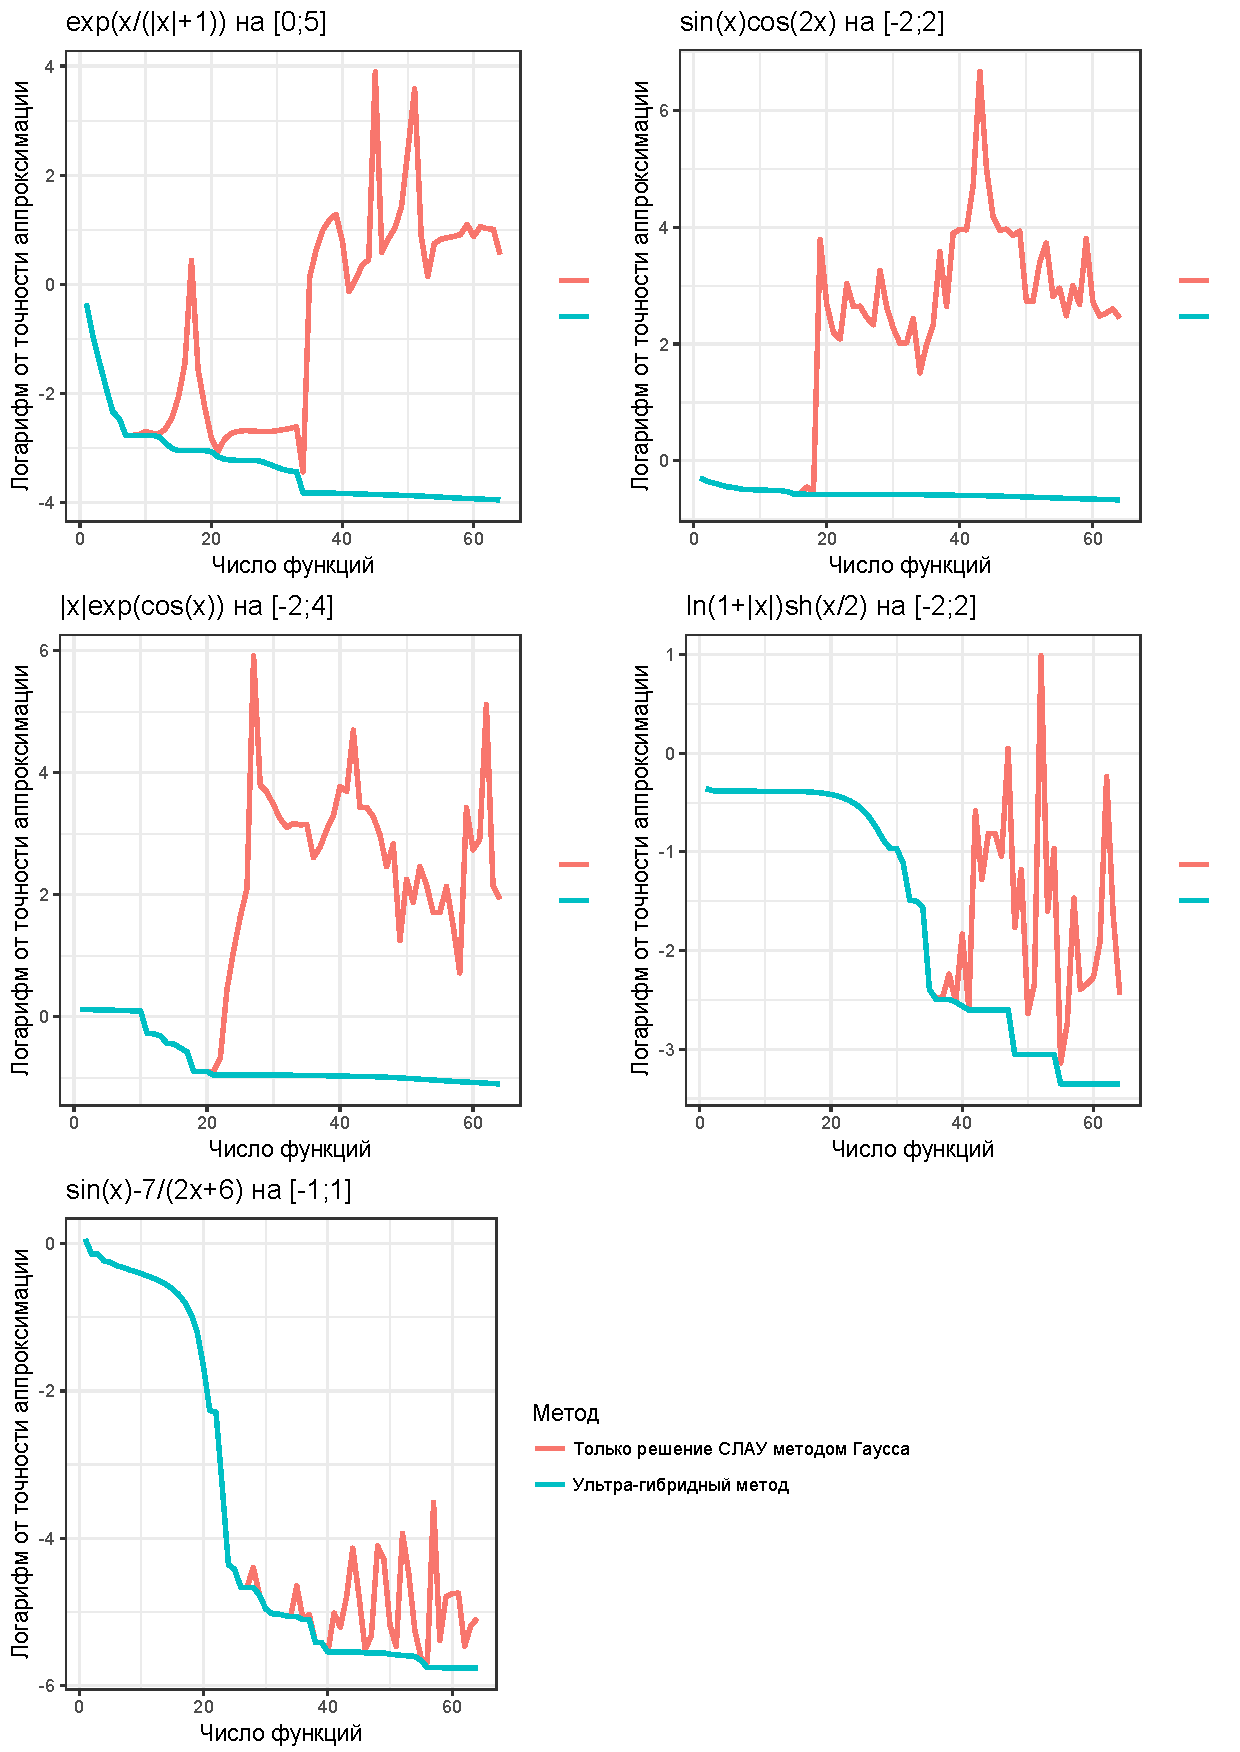
\includegraphics[width=0.9\linewidth]{log.pdf}
  }
   \caption{Аппроксимация логарифмами}
    \label{log}
\end{figure}


Алгоритм не гарантирует нахождения максимально точного решения системы, но гарантирует устойчивое невозрастание невязки при росте размерности системы. Сложность алгоритма равна $O(N^4)$, но это не вносит видимого отрицательного вклада в производительность, поскольку системы с плохо обусловленными матрицами, как правило, не используют слишком большими, вдобавок конкретно в исходной задаче на порядок дольше будут вычисляться коэффициенты СЛАУ.

Также следует отметить, что ещё не встречалось примера, когда ультра-гибрид приводил к значительно более точной аппроксимации в сравнении с классическим вариантом при наименьшей невязке (из графиков \ref{mon}-\ref{log} видно, что кривая минимальное значение ультра-гибрида не находится значительно ниже минимального значения классического метода) Ценность ультра-гибрида будет показана позже.

\section{Примеры решения ОЗГ}
В этом разделе приводятся примеры решения ОЗГ для разных областей и плотностей.
В качестве областей брались области, ограниченные кривыми из рисунков (\ref{kvci}) и (\ref{tros}) (названия соответственно CIRCLE, TRIANGLE, SQUARE и EDGE) с той же параметризацией, возможно, слегка подкорректированной для возможности интегрирования описанным ранее методом; радиус кривых по умолчанию равен 0.5.
В качестве граничных функций брались как гармонические, так и негармонические, чтобы продемонстрировать, как метод будет приближённо искать их гармоническую часть и как много найденная часть вносит в саму аппроксимируемую функцию; функции были следующими ($x,y$ --- координаты точки на плоскости, $\alpha$ --- аргумент точки относительно начала координат):
\begin{equation*}
  f_1=x+y,
\end{equation*}
\begin{equation*}
  f_2=\sin (y) \left(e^x+e^{-x}\right),
\end{equation*}
\begin{equation*}
  f_3=3x+6y+\sqrt{x^2+y^2}+\dfrac{1}{2}y^2,
\end{equation*}
\begin{equation*}
  f_4=1.5,
\end{equation*}
\begin{equation*}
  f_5=x^2-y^2,
\end{equation*}
\begin{equation*}
  f_6=f_1(x,y) \cdot e^{x-y}=(x+y)e^{x-y},
\end{equation*}
\begin{equation*}
  f_7=
  \begin{cases}
    -\frac{1}{2},& -\pi \leq \alpha < -\frac{2 \pi}{3} \\
    0,& -\frac{2 \pi}{3} < \alpha \leq -\frac{\pi}{3} \\
    \frac{1}{2},& -\frac{\pi}{3} < \alpha \leq \frac{\pi}{2}  \\
    -\frac{1}{2},&\text{иначе}
  \end{cases},
\end{equation*}
\begin{equation*}
  f_8=f_3+f_7,
\end{equation*}
\begin{equation*}
  f_9= e^x( \cos y +3\sin  y),
\end{equation*}
\begin{equation*}
  f_{10}= \sum_{i=1}^{5} f_i,
\end{equation*}
\begin{equation*}
  f_{11}= -\ln (|x-z_1|).
\end{equation*}

\subsection{Пояснения для рисунков}
Контуры из рисунков (\ref{kvci}) и (\ref{tros}) обозначаются за $\partial Q$, $Q$ --- область, ограниченная одним из этих контуров,
$L$ --- подобный $\partial Q$ контур радиуса $r$, причём $Q$ содержится внутри области, им ограниченной. Радиус $r$ может меняться от собственно радиуса $\partial Q$ до некоторого фиксированного значения.

Приближённое значение плотности $\rho$ равно
\begin{equation*}
  \tilde{\rho} = \sum_i c_i \alpha_i,
\end{equation*}
где $\alpha_i$ --- базисный потенциал от $i$-й точки.
Точек $z_i$ выбрано некоторое количество и располагаются они равномерно по кривой $L_p$, подобной $L$, но большего радиуса, с небольшими случайными отклонениями по нормали от $L$.

На кривой $L$ известна функция $V_f(x)=\V{f}$, где $f$ --- одна из перечисленных ранее тестовых функций.
Тогда коэффициенты $c_i$ из $\tilde{\rho}$ находятся как компоненты решения задачи минимизации:
\begin{equation*}
  F(c_1,\dots,c_i,\dots,c_n)=||V_f-V_{\tilde{\rho} } ||_{L_2(L)}\rightarrow \min.
\end{equation*}

Значение $||V_f-V_{\tilde{\rho} } ||_{L_2(L)}$ есть точность аппроксимации потенциала на $L$.
Значение $||\rho-\tilde{\rho} ||_{L_2(Q)}$ есть точность аппроксимации плотности на области $Q$.
Цель метода --- осуществить аппроксимацию на $Q$.

\subsection{2D-графики}
По известному алгоритму для разных областей $Q$ и разных плотностей $\rho=f_i,i=1,2,\dots,10$ были найдены приближённые плотности $\tilde{\rho}$.
На следующих графиках (рисунки \ref{gbeg}-\ref{hexampl}) показаны функции $\rho, \tilde{\rho}$ (плотности) и $V_{\rho},V_{\tilde{\rho}}$ (исходники) на кривых $L$, графики рисуются по отрезку параметризации $L$, число базисных потенциалов $n$ зафиксировано.
Под качеством аппроксимации имеются в виду значения $||\rho-\tilde{\rho} ||_{L_2(Q)}$ и $||V_f-V_{\tilde{\rho} } ||_{L_2(L)}$; в скобках обозначены те же значения для случая, когда $L$ совпадает с $\partial Q$ (когда радиус этих двух контуров одинаков).

\begin{figure}[h] 
  \center{\begin{minipage}[h]{\linewidth} 
  \center{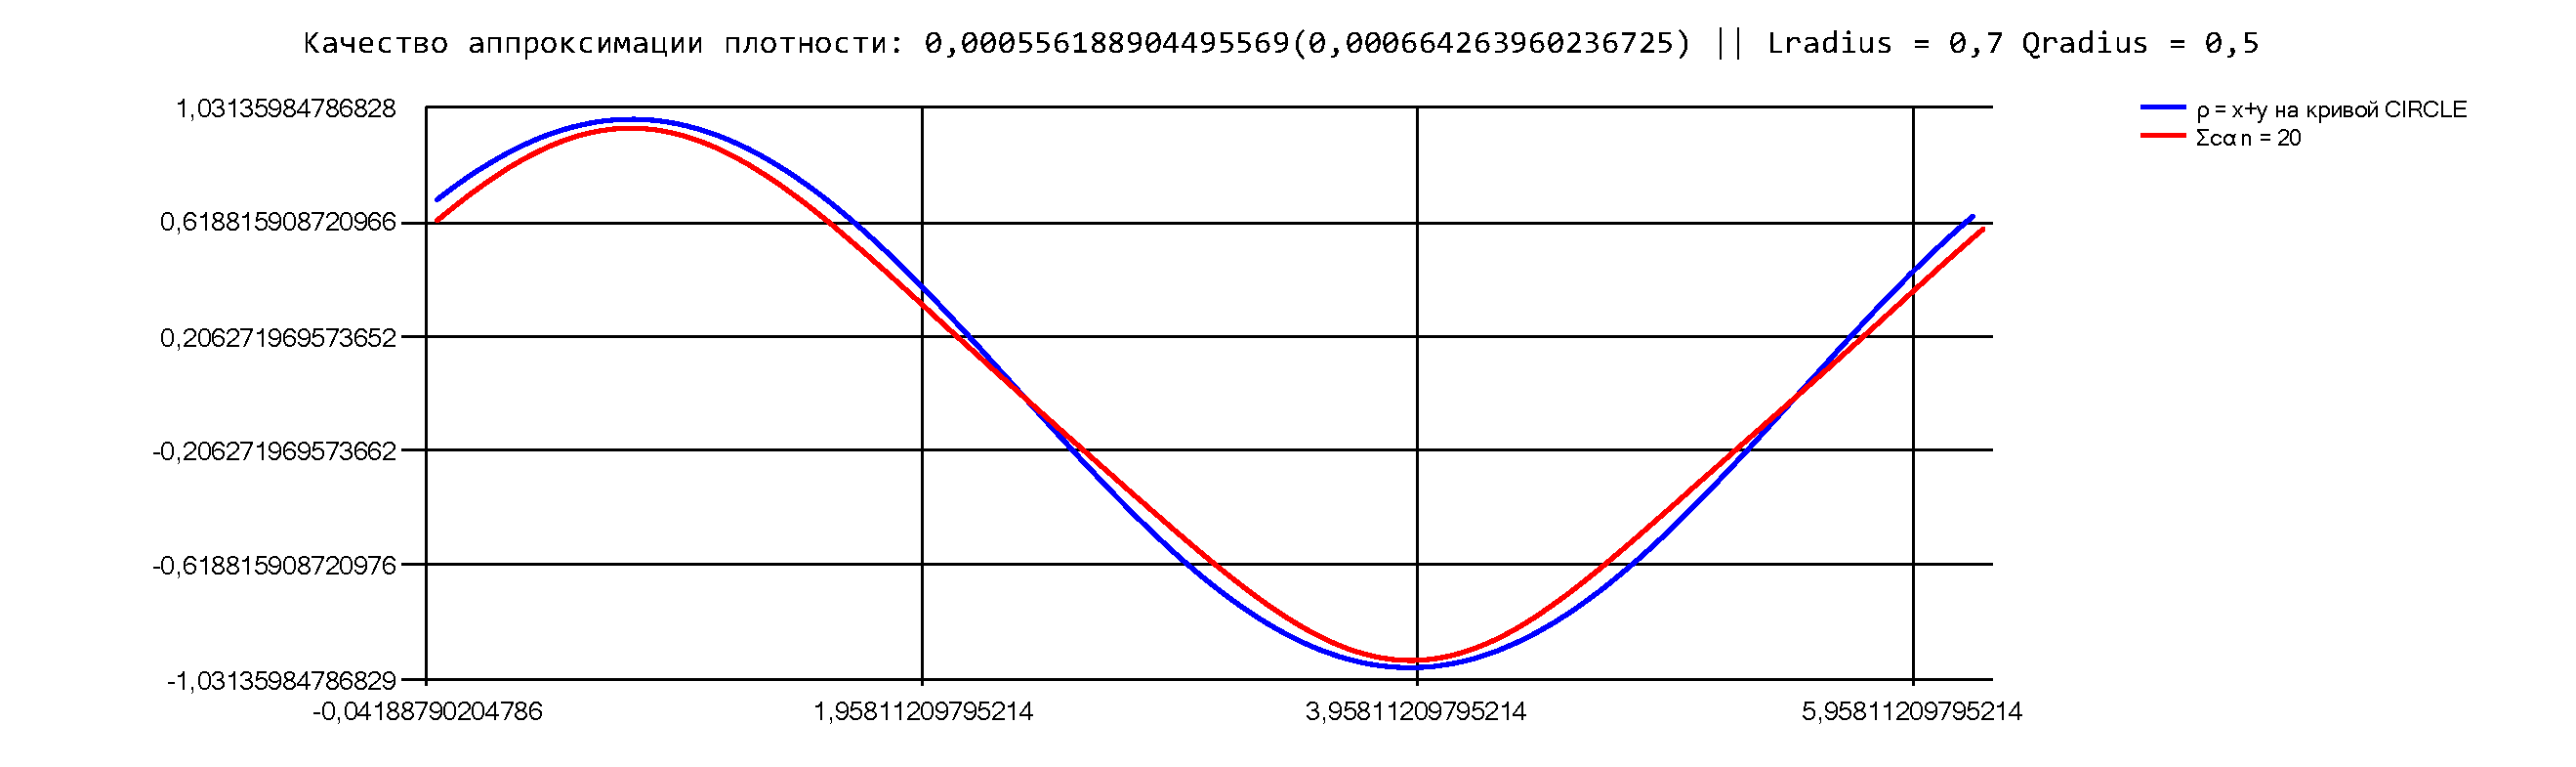
\includegraphics[width=0.8\linewidth]{d1.pdf} \\ для плотности} 
  \end{minipage}} 
  \vfill 
  \center{\begin{minipage}[h]{\linewidth} 
  \center{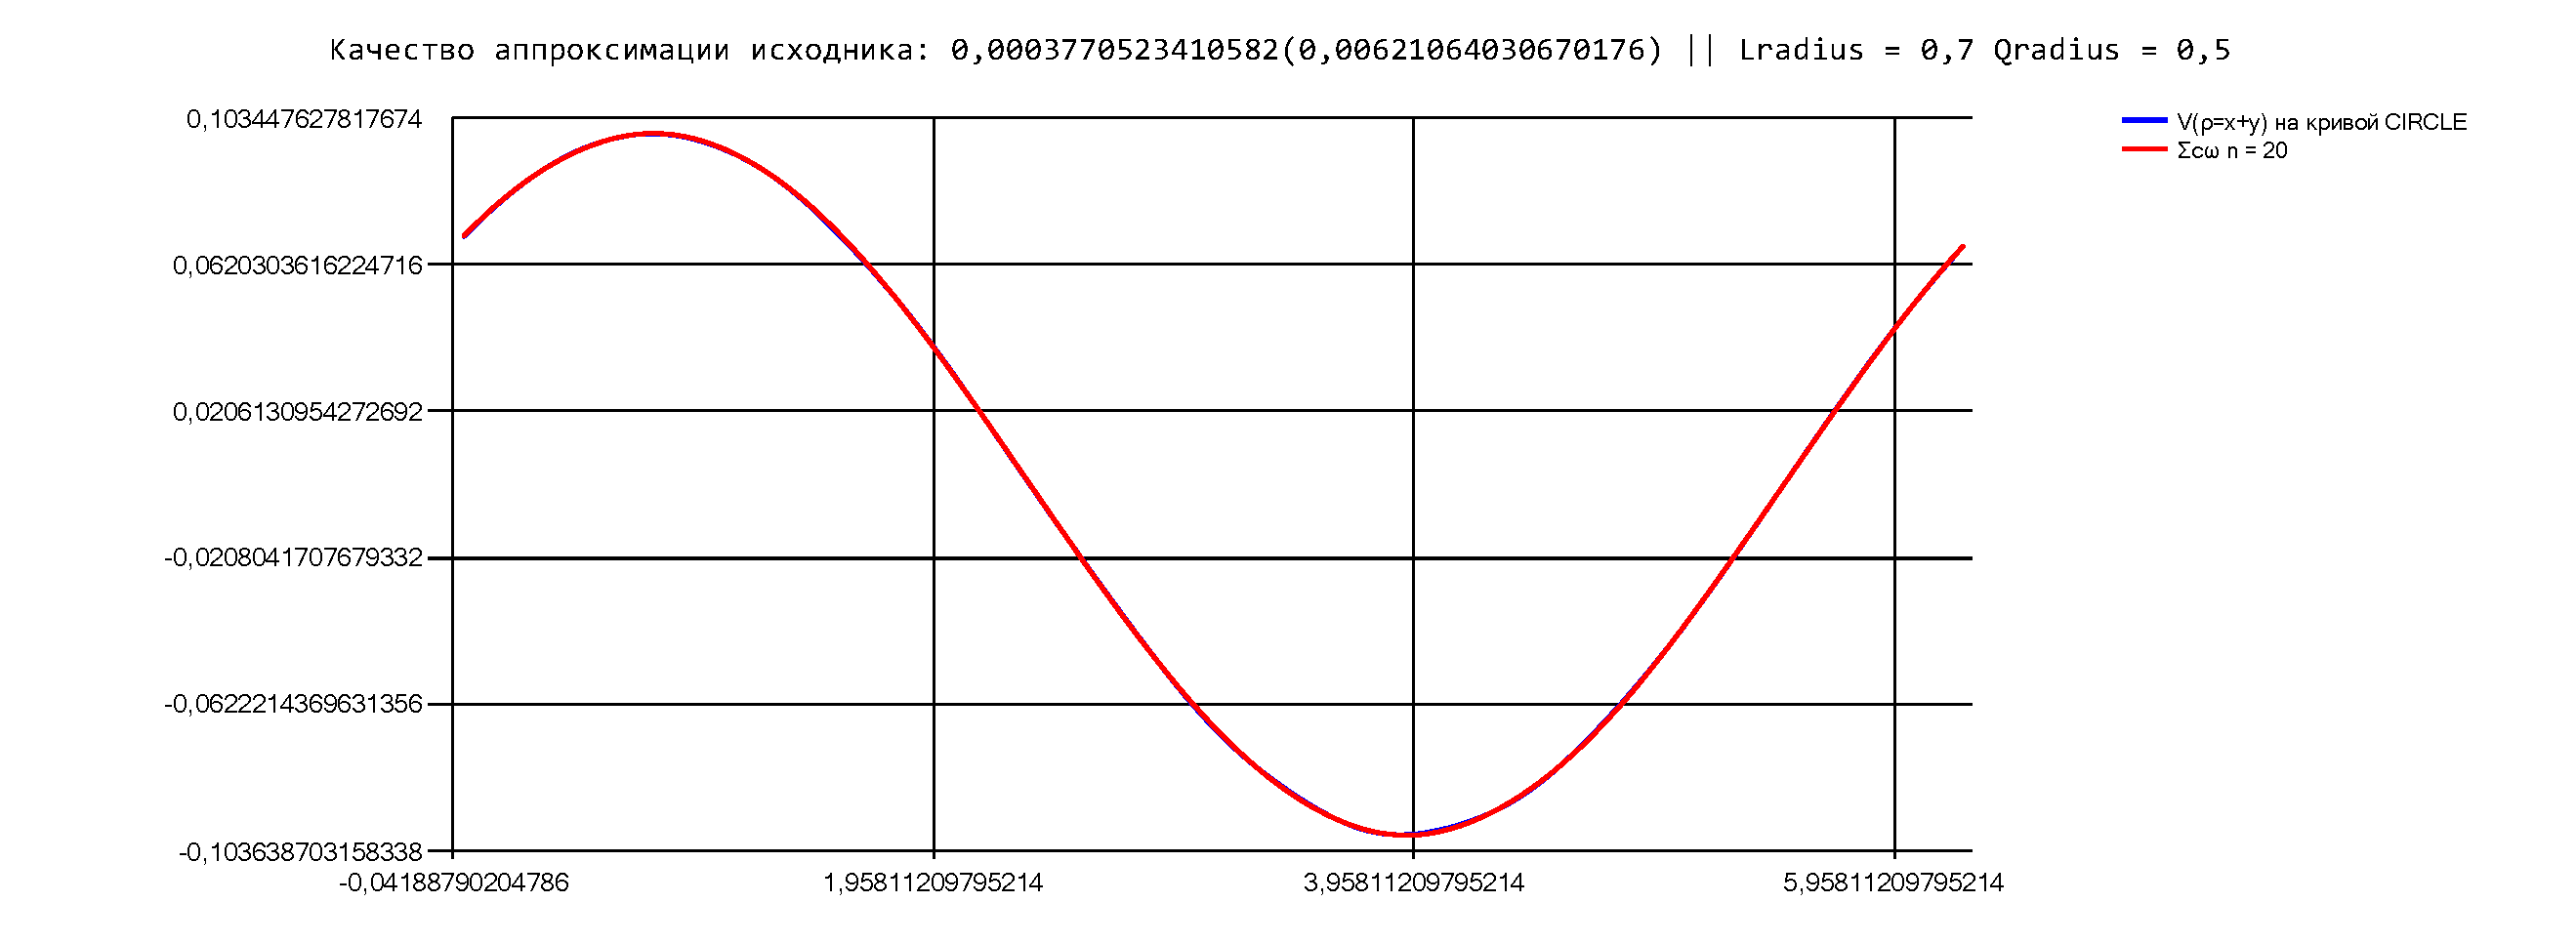
\includegraphics[width=0.8\linewidth]{v1.pdf} \\ для потенциала} 
  \end{minipage}} 
  \caption{Один из результатов работы алгоритма} 
  \label{gbeg} 
  \end{figure}

  \begin{figure}[h] 
    \center{\begin{minipage}[h]{\linewidth} 
    \center{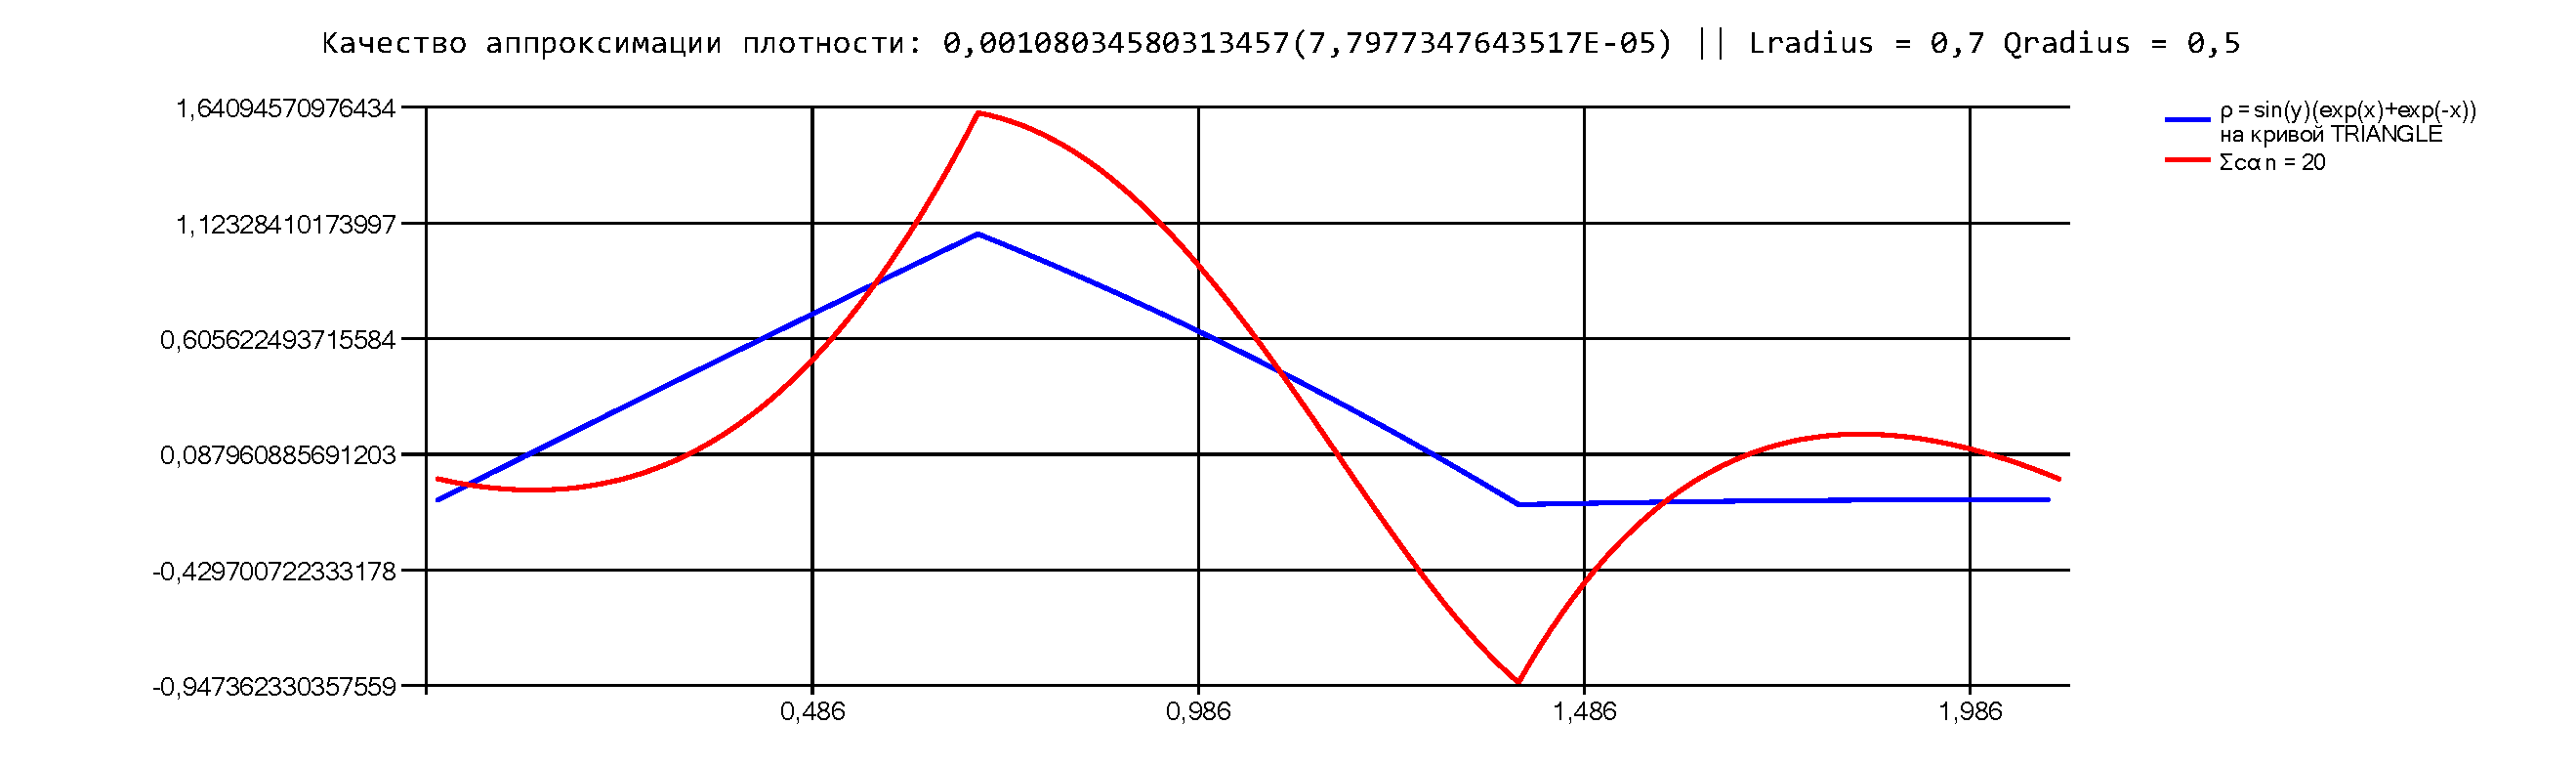
\includegraphics[width=0.8\linewidth]{d2.pdf} \\ для плотности} 
    \end{minipage}} 
    \vfill 
    \center{\begin{minipage}[h]{\linewidth} 
    \center{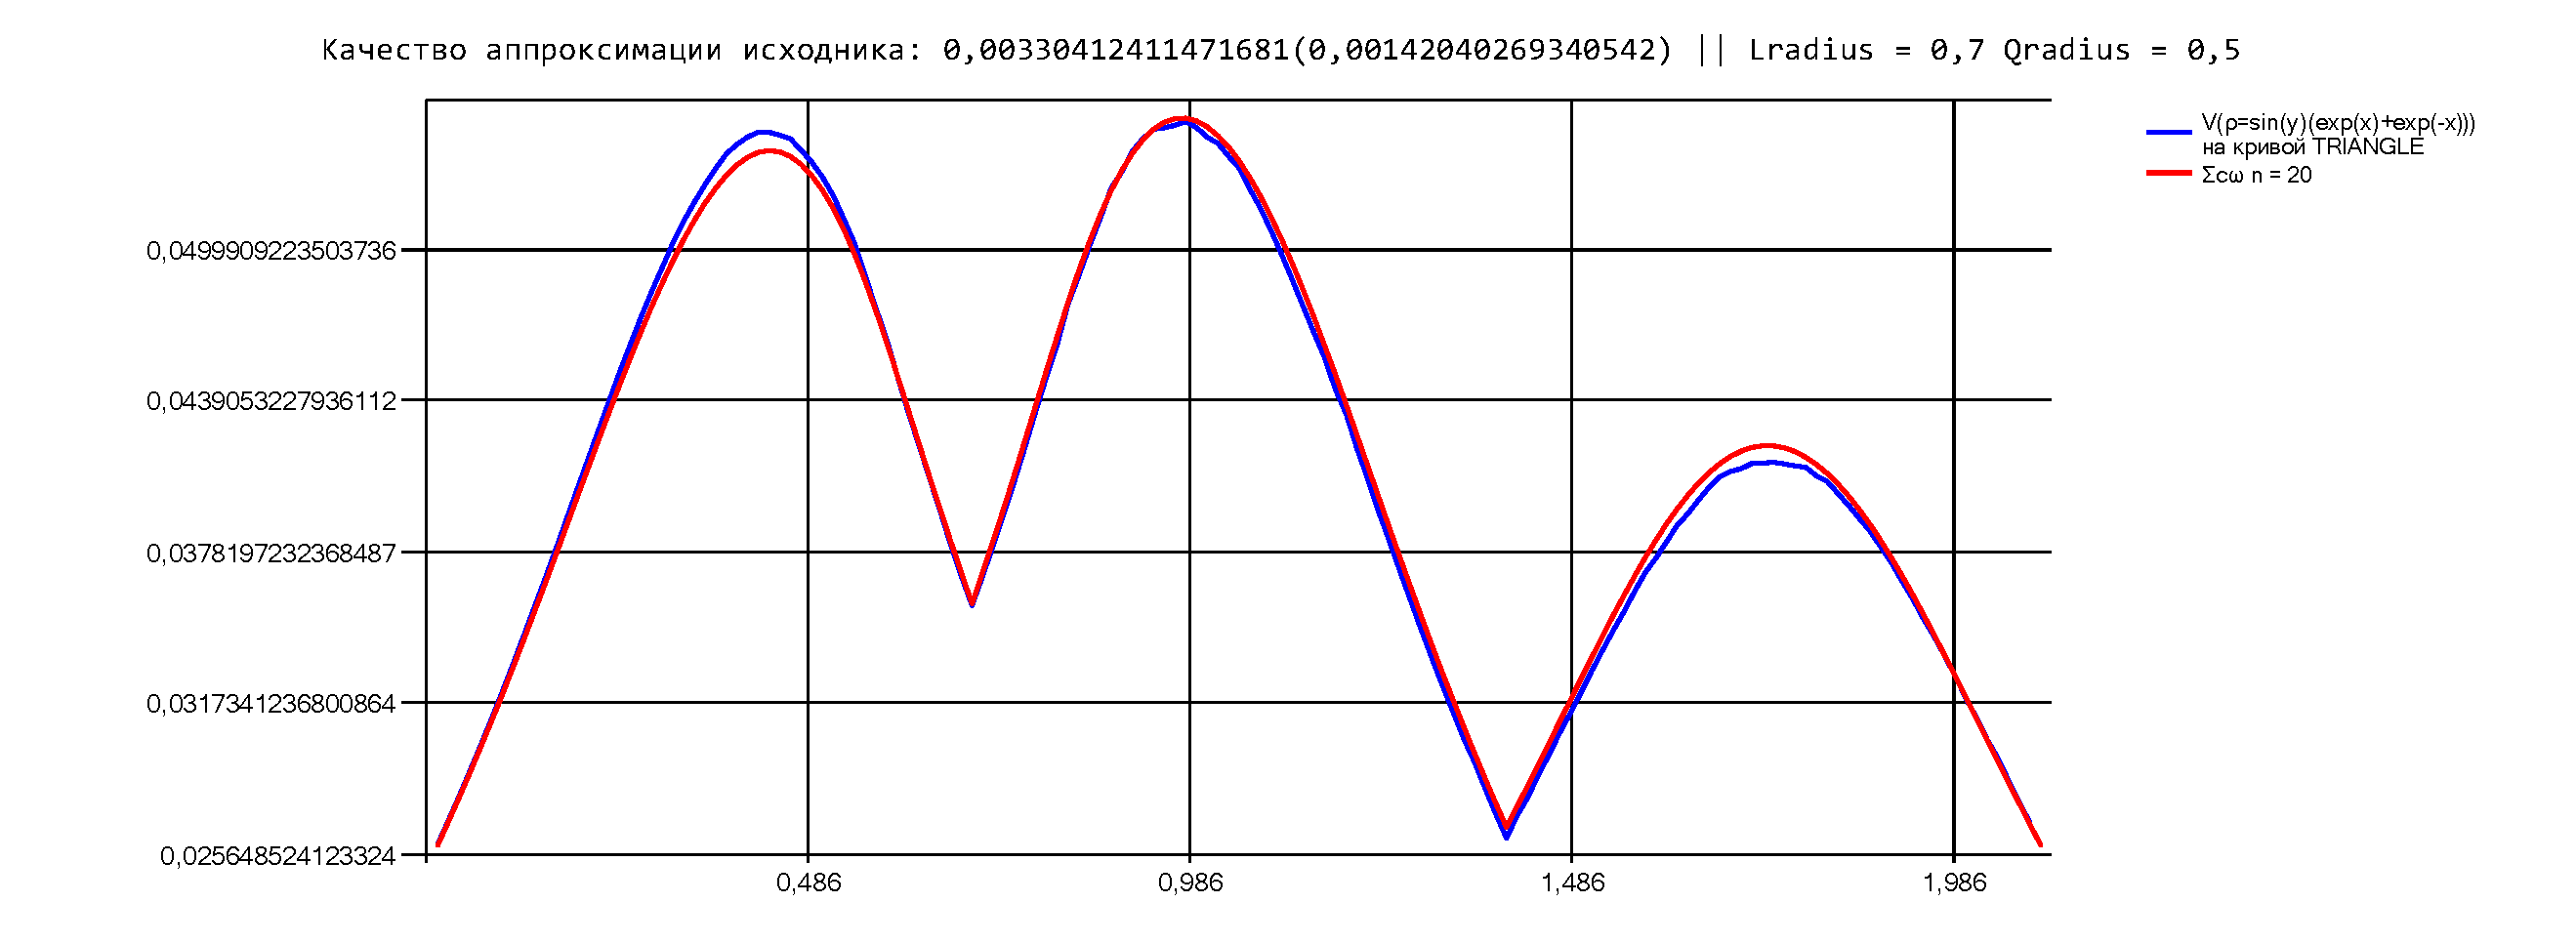
\includegraphics[width=0.8\linewidth]{v2.pdf} \\ для потенциала} 
    \end{minipage}} 
    \caption{Один из результатов работы алгоритма} 
    \label{ris:image1} 
    \end{figure}

    \begin{figure}[h] 
      \center{\begin{minipage}[h]{\linewidth} 
      \center{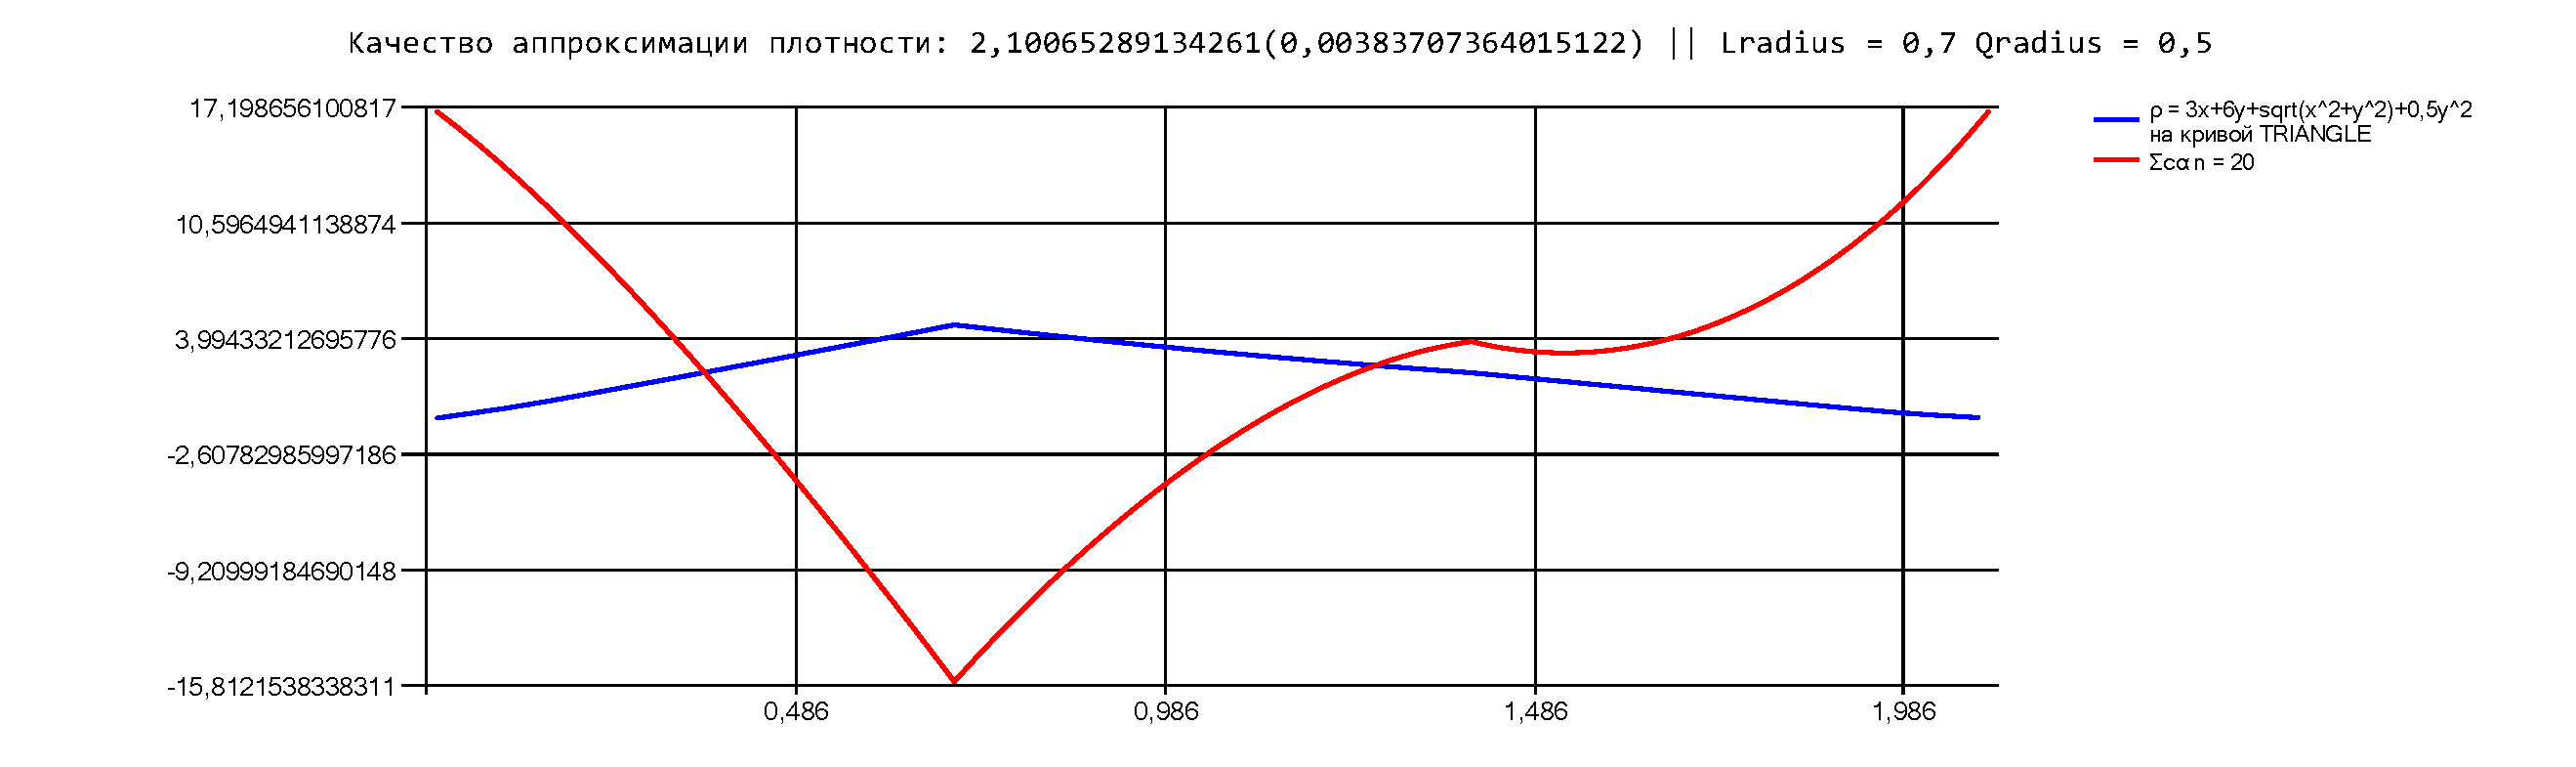
\includegraphics[width=0.8\linewidth]{d3.pdf} \\ для плотности} 
      \end{minipage}} 
      \vfill 
      \center{\begin{minipage}[h]{\linewidth} 
      \center{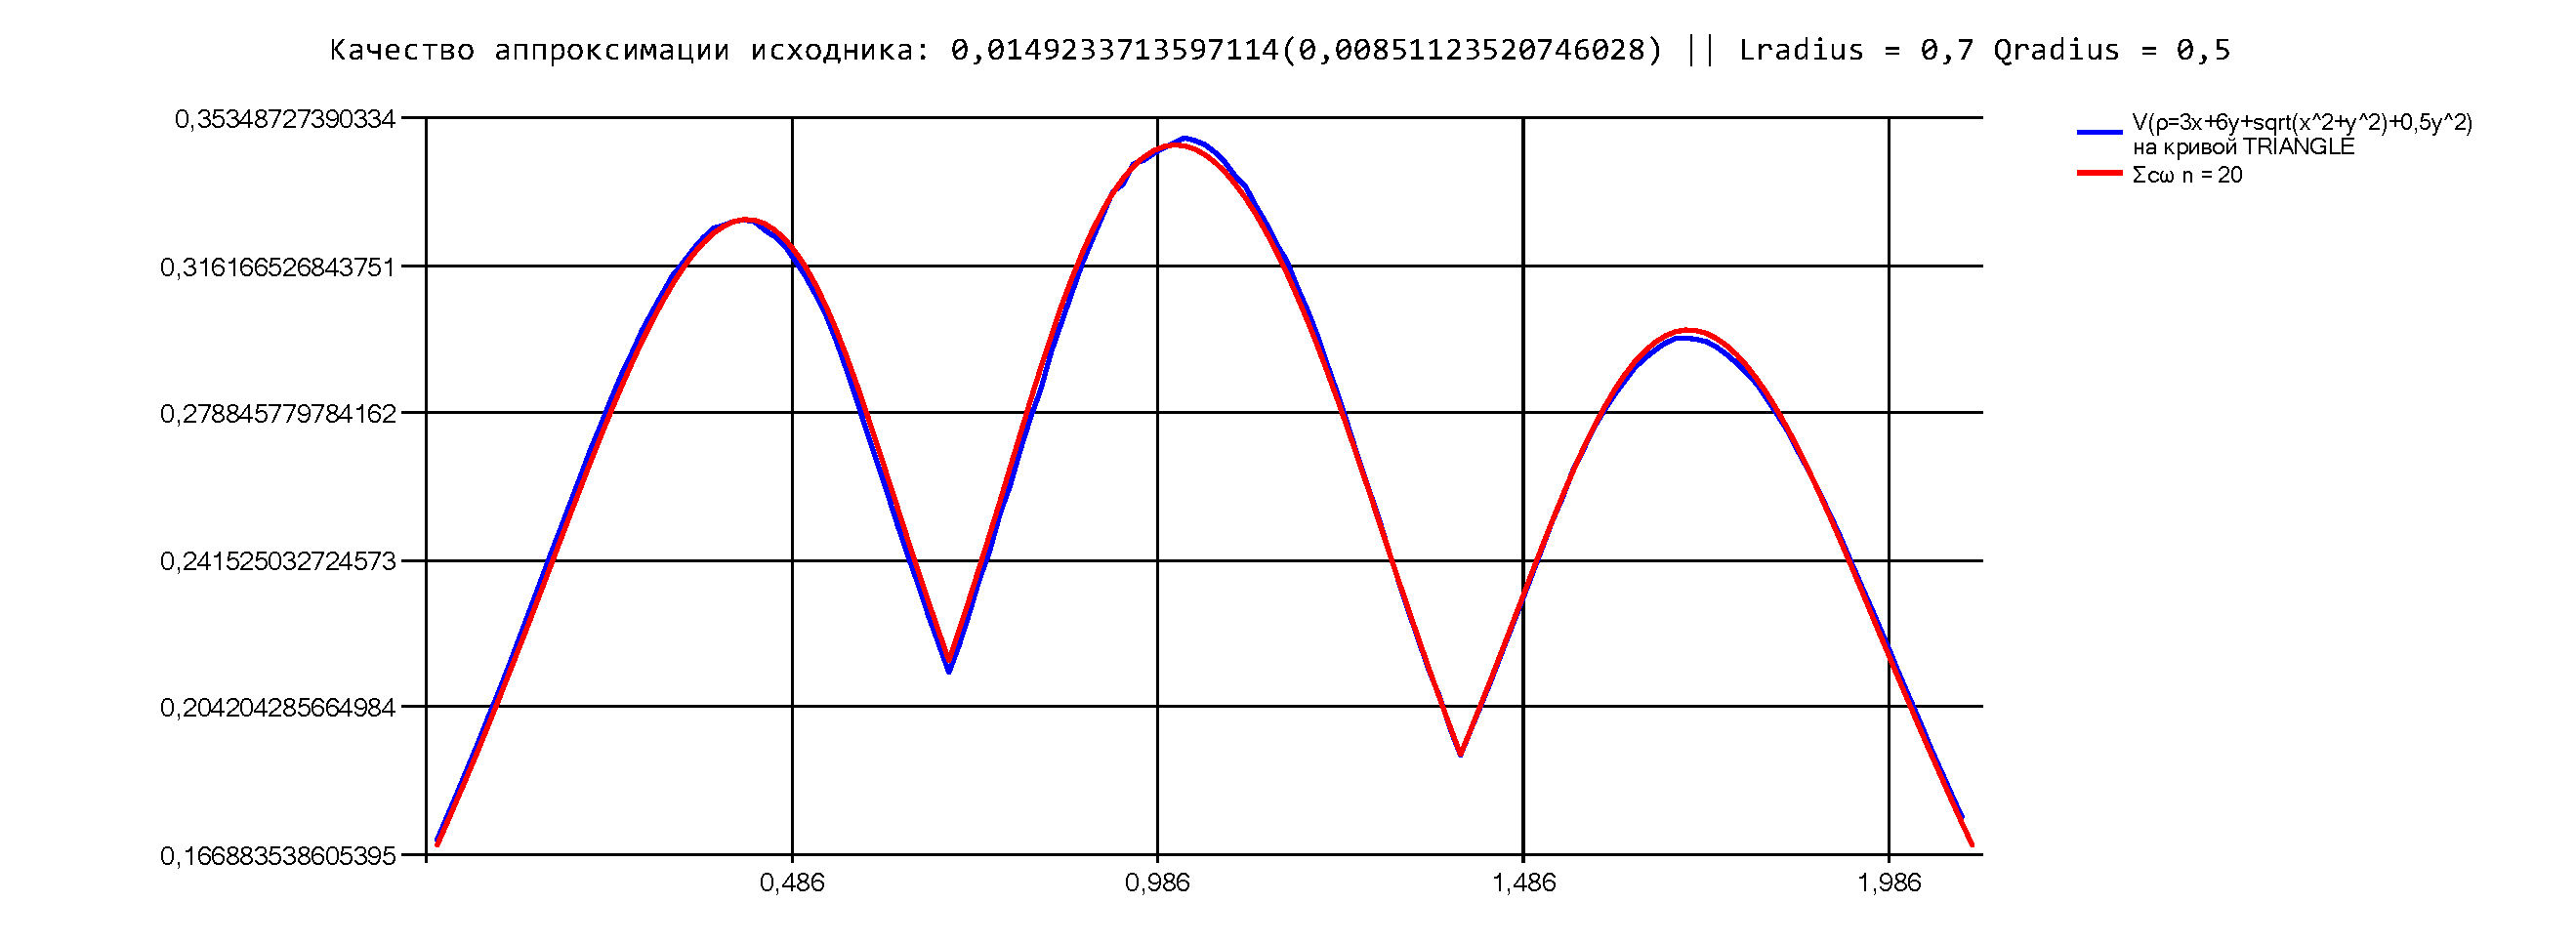
\includegraphics[width=0.8\linewidth]{v3.pdf} \\ для потенциала} 
      \end{minipage}} 
      \caption{Один из результатов работы алгоритма} 
      \label{ris:image1} 
      \end{figure}

      \begin{figure}[h] 
        \center{\begin{minipage}[h]{\linewidth} 
        \center{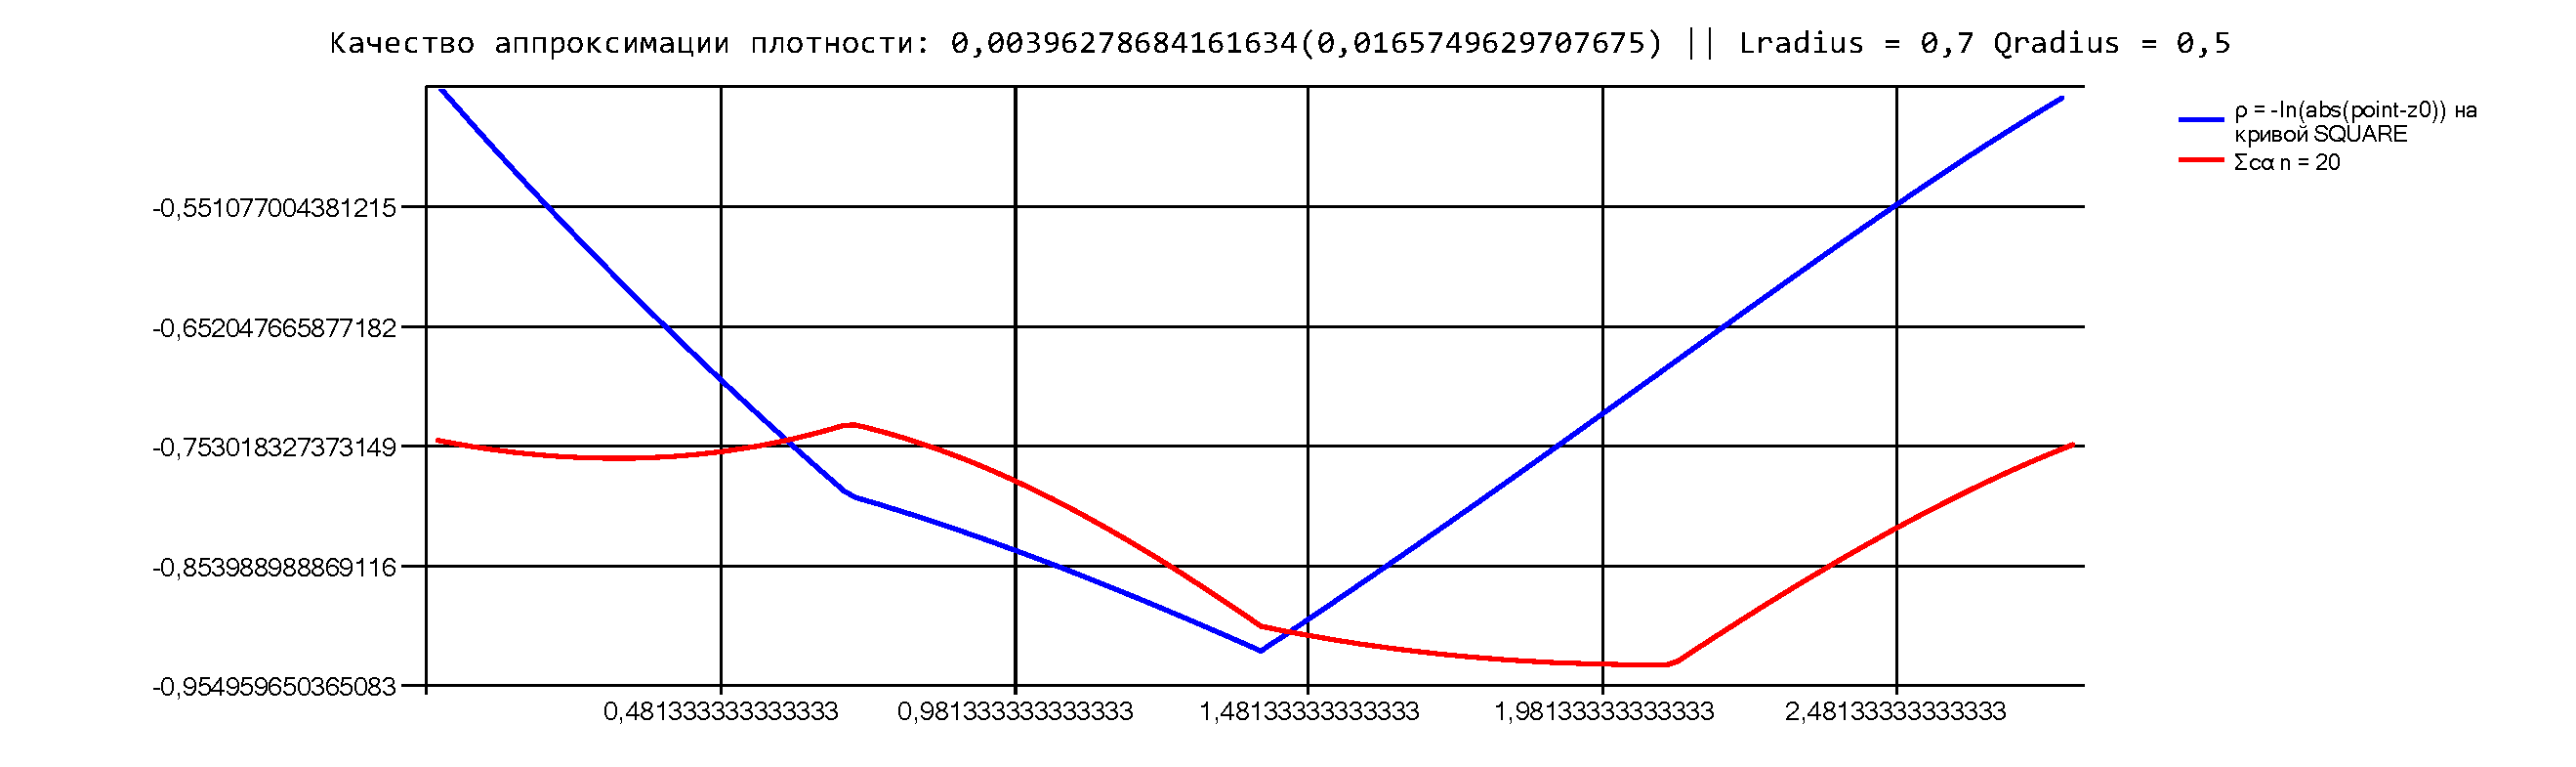
\includegraphics[width=0.8\linewidth]{d4.pdf} \\ для плотности} 
        \end{minipage}} 
        \vfill 
        \center{\begin{minipage}[h]{\linewidth} 
        \center{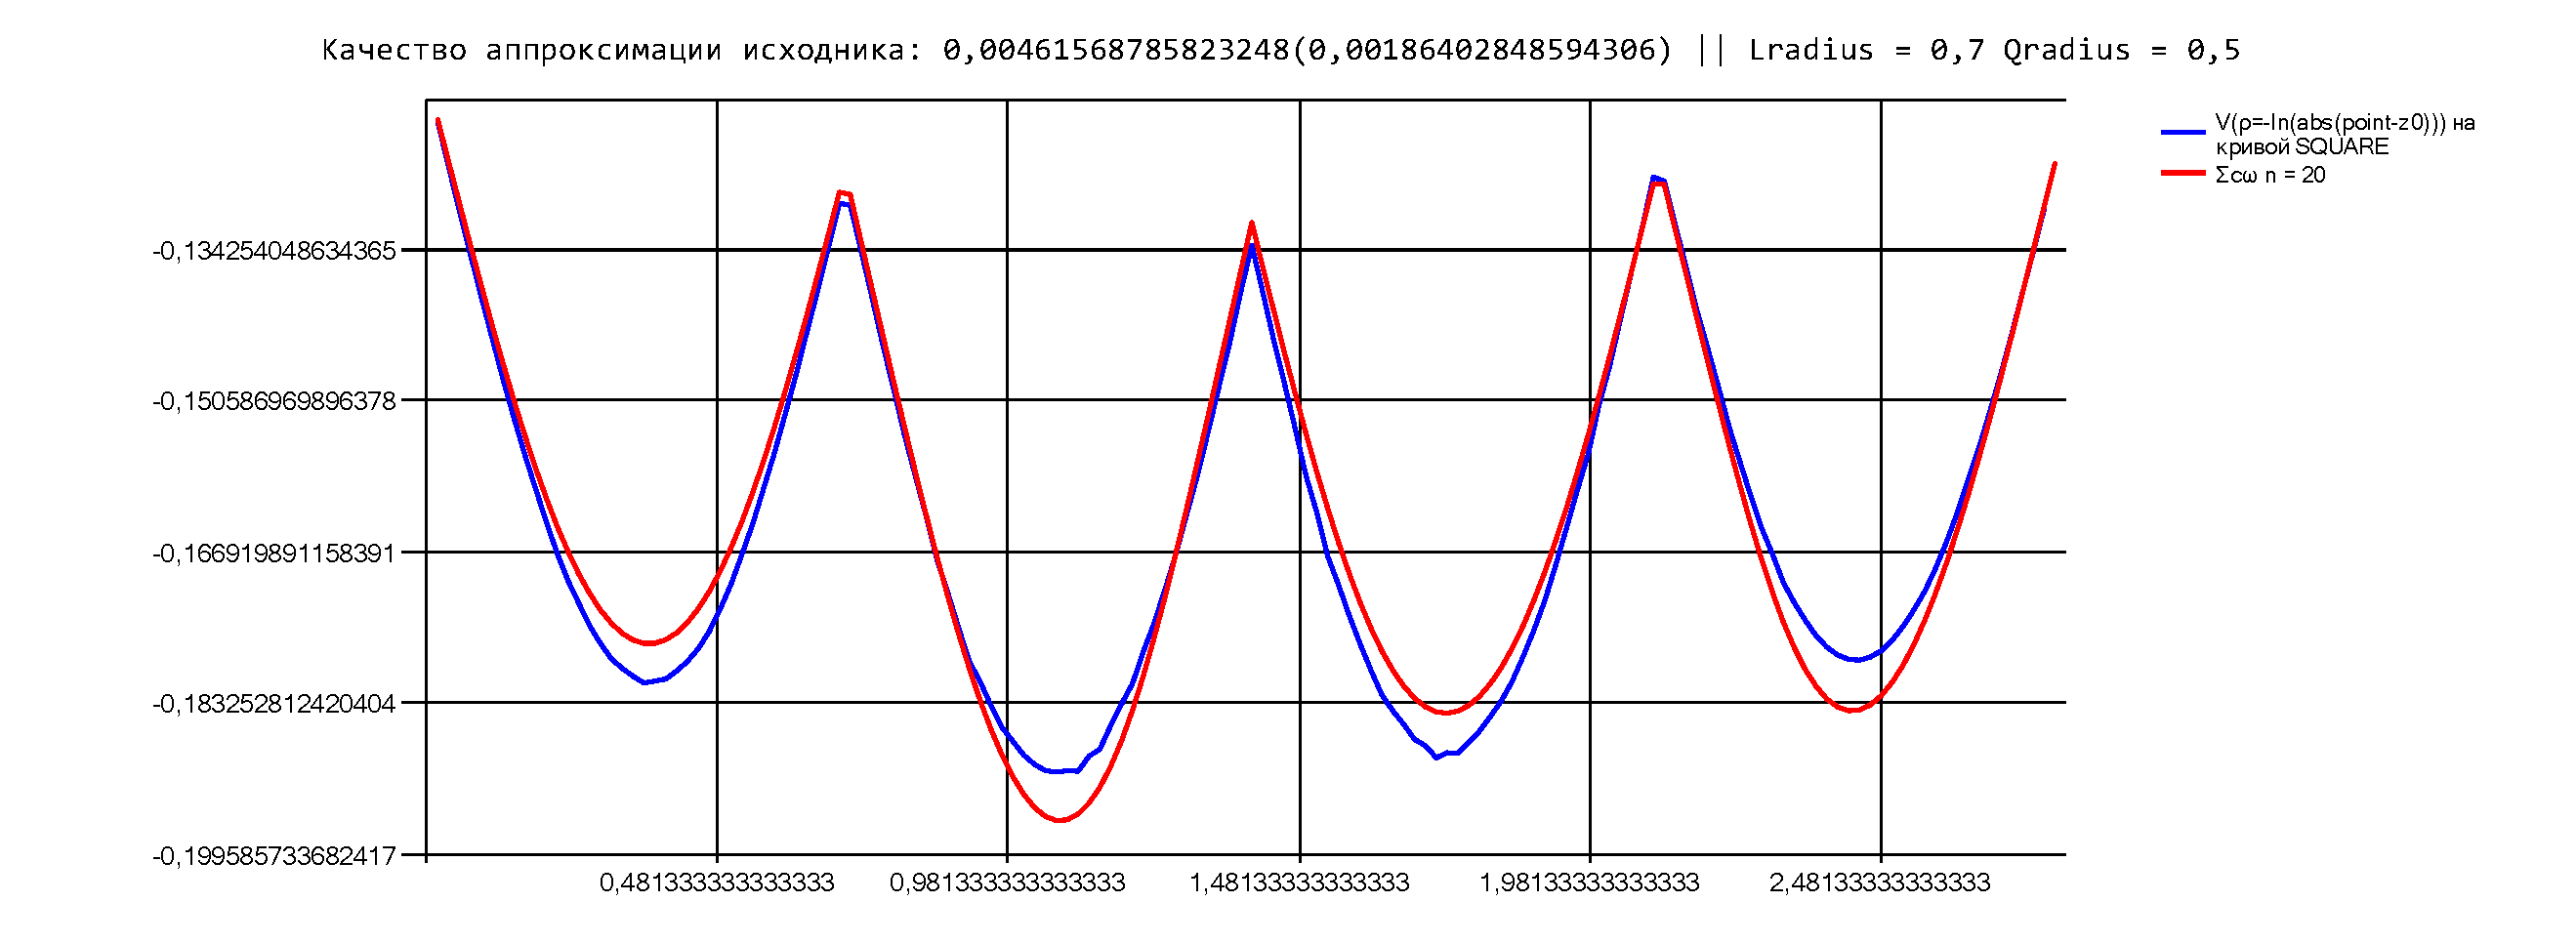
\includegraphics[width=0.8\linewidth]{v4.pdf} \\ для потенциала} 
        \end{minipage}} 
        \caption{Один из результатов работы алгоритма} 
        \label{ris:image1} 
        \end{figure}

        \begin{figure}[h] 
          \center{\begin{minipage}[h]{\linewidth} 
          \center{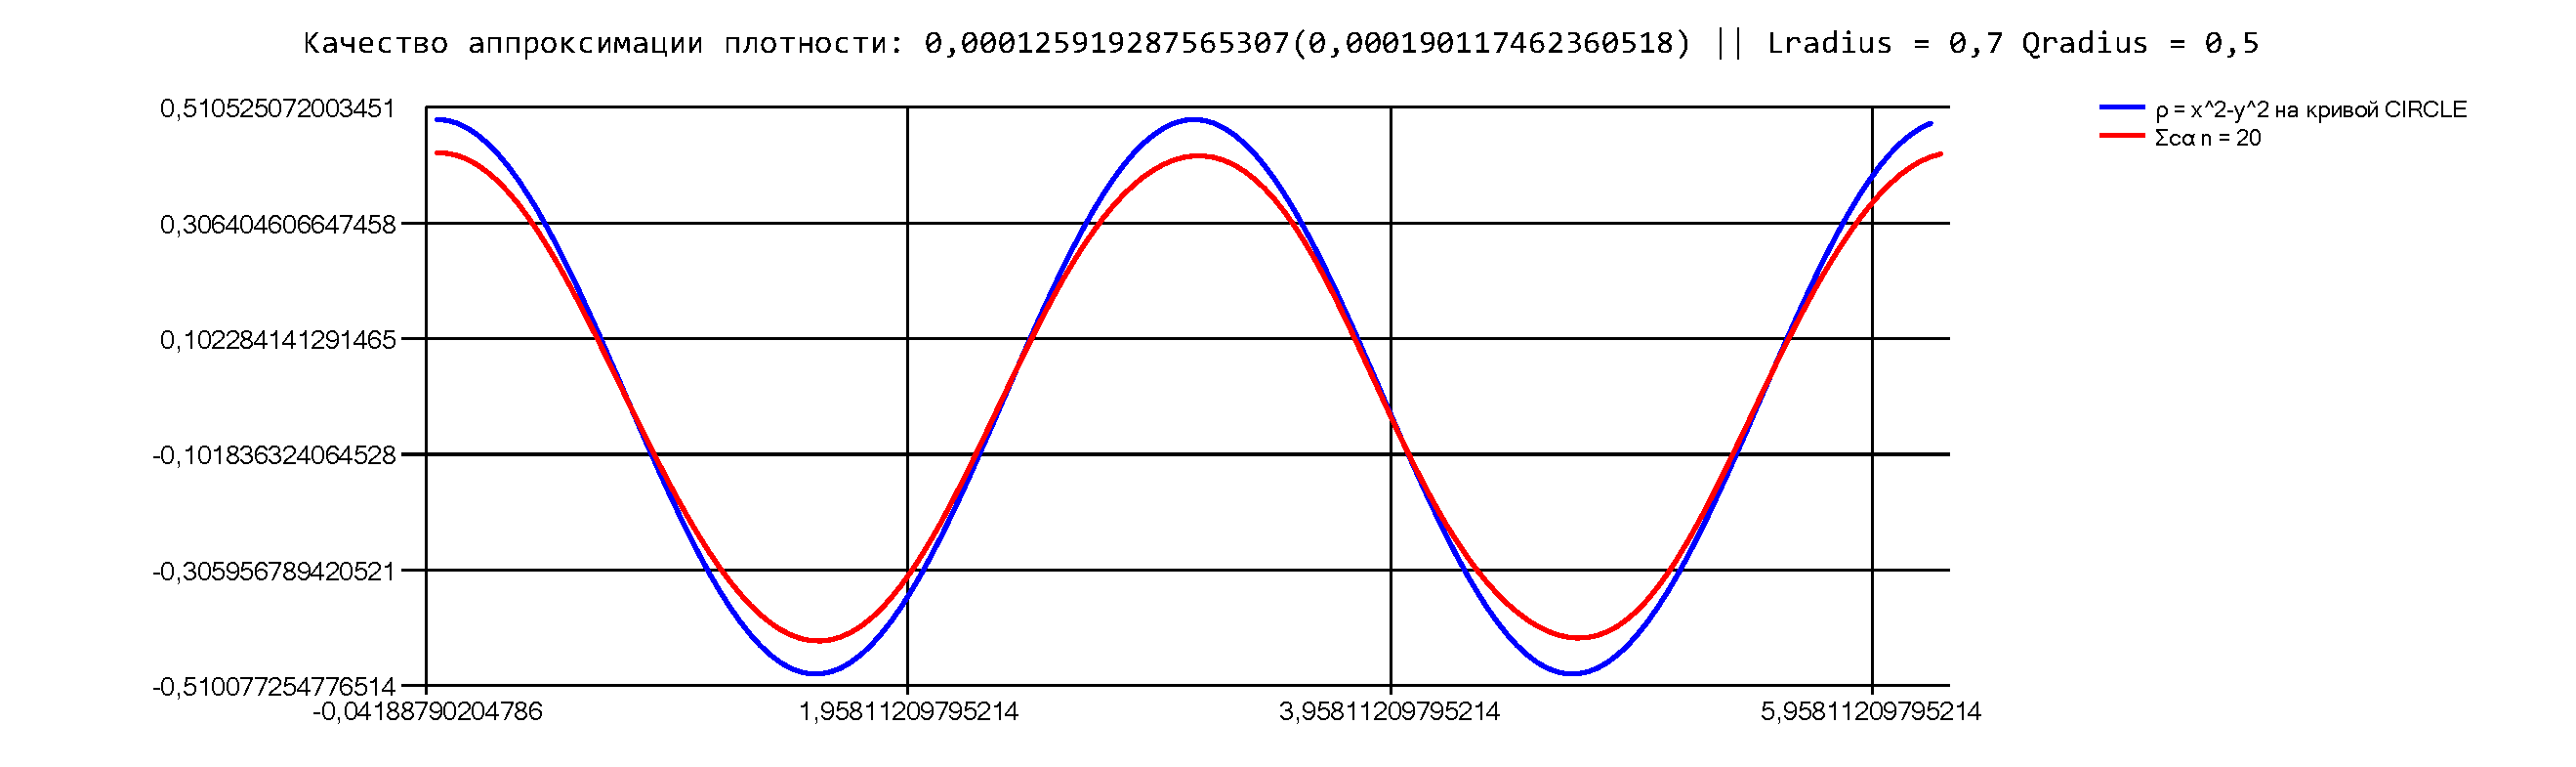
\includegraphics[width=0.8\linewidth]{d5.pdf} \\ для плотности} 
          \end{minipage}} 
          \vfill 
          \center{\begin{minipage}[h]{\linewidth} 
          \center{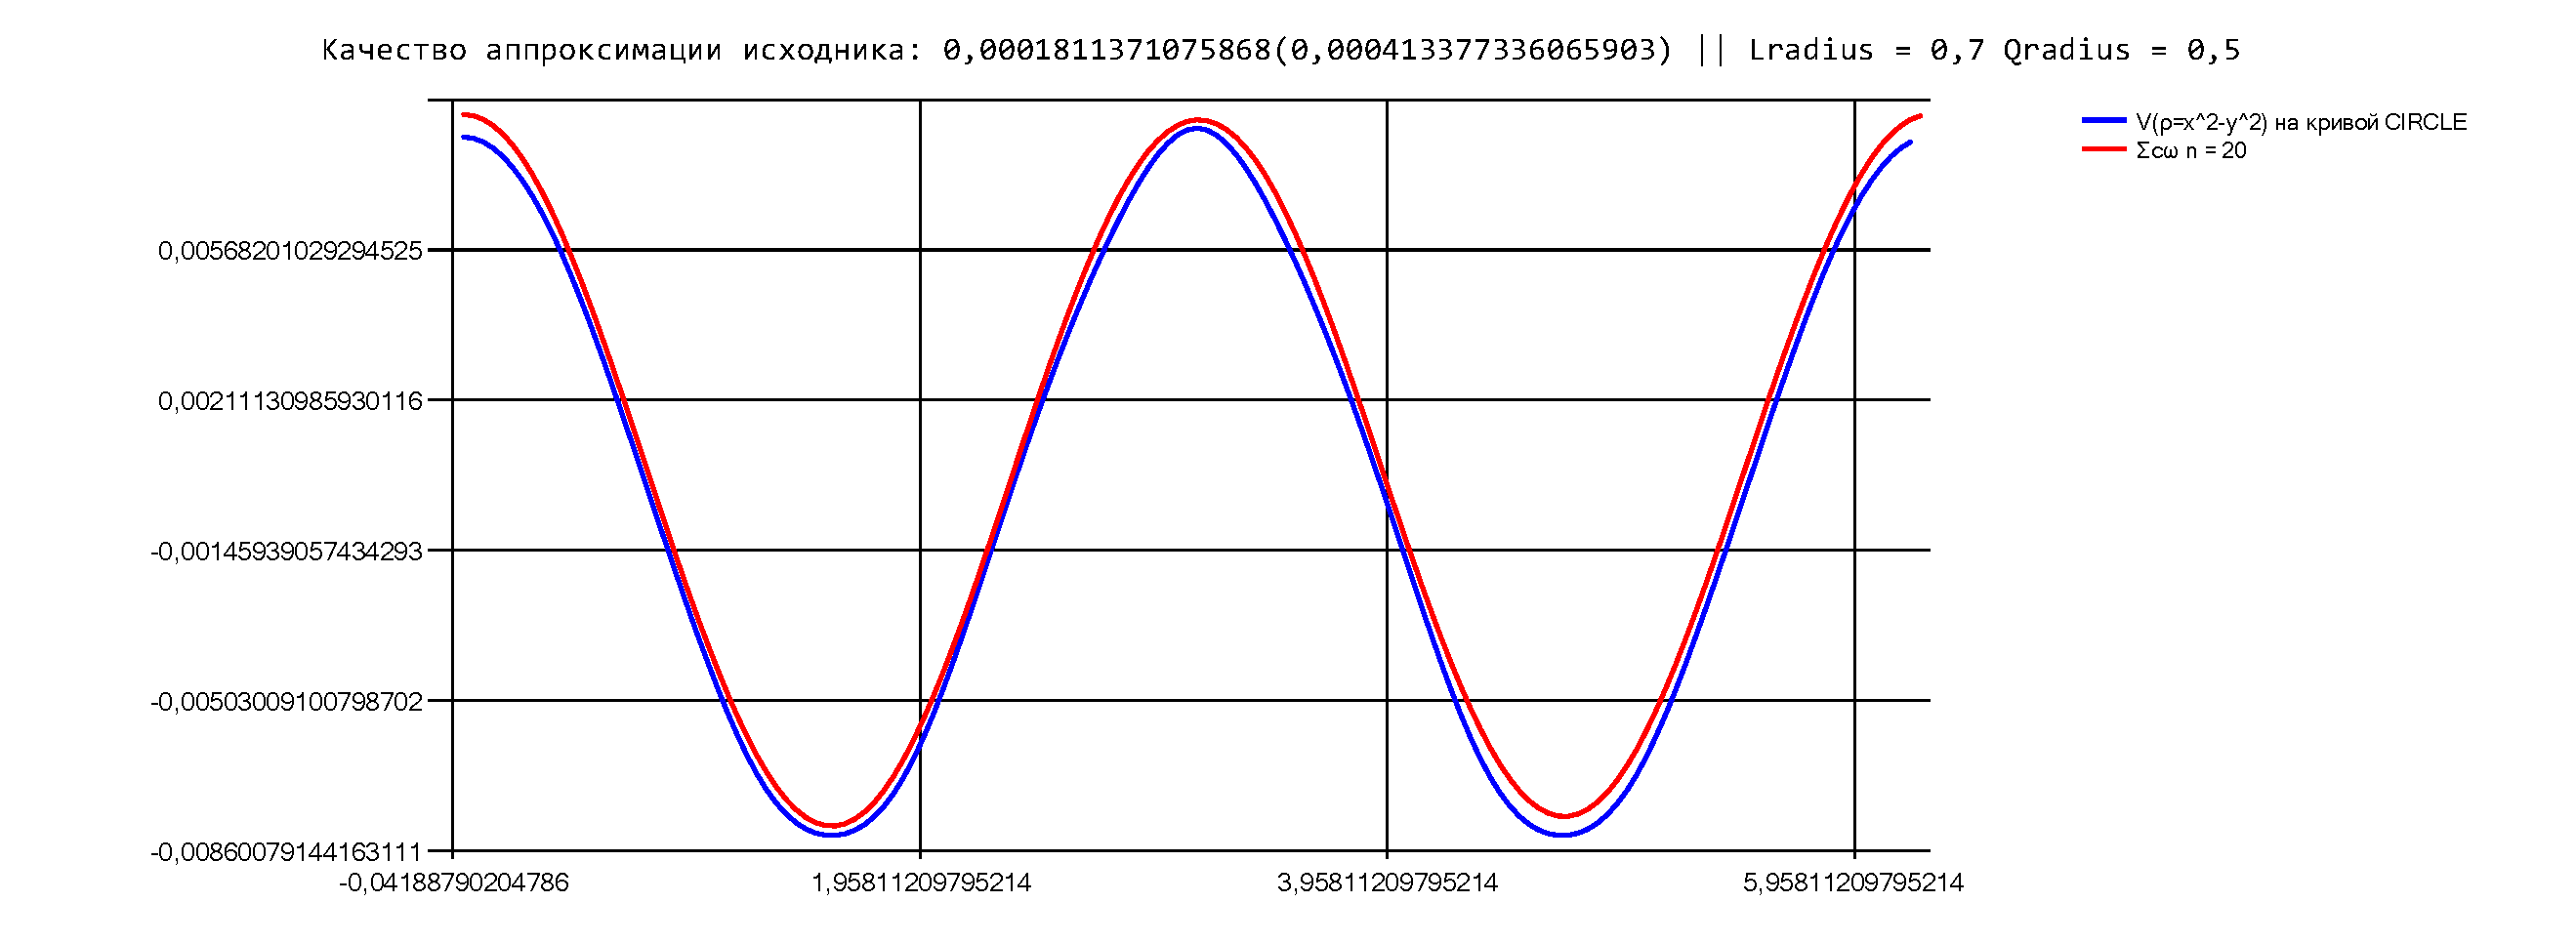
\includegraphics[width=0.8\linewidth]{v5.pdf} \\ для потенциала} 
          \end{minipage}} 
          \caption{Один из результатов работы алгоритма} 
          \label{ris:image1} 
          \end{figure}

          \begin{figure}[h] 
            \center{\begin{minipage}[h]{\linewidth} 
            \center{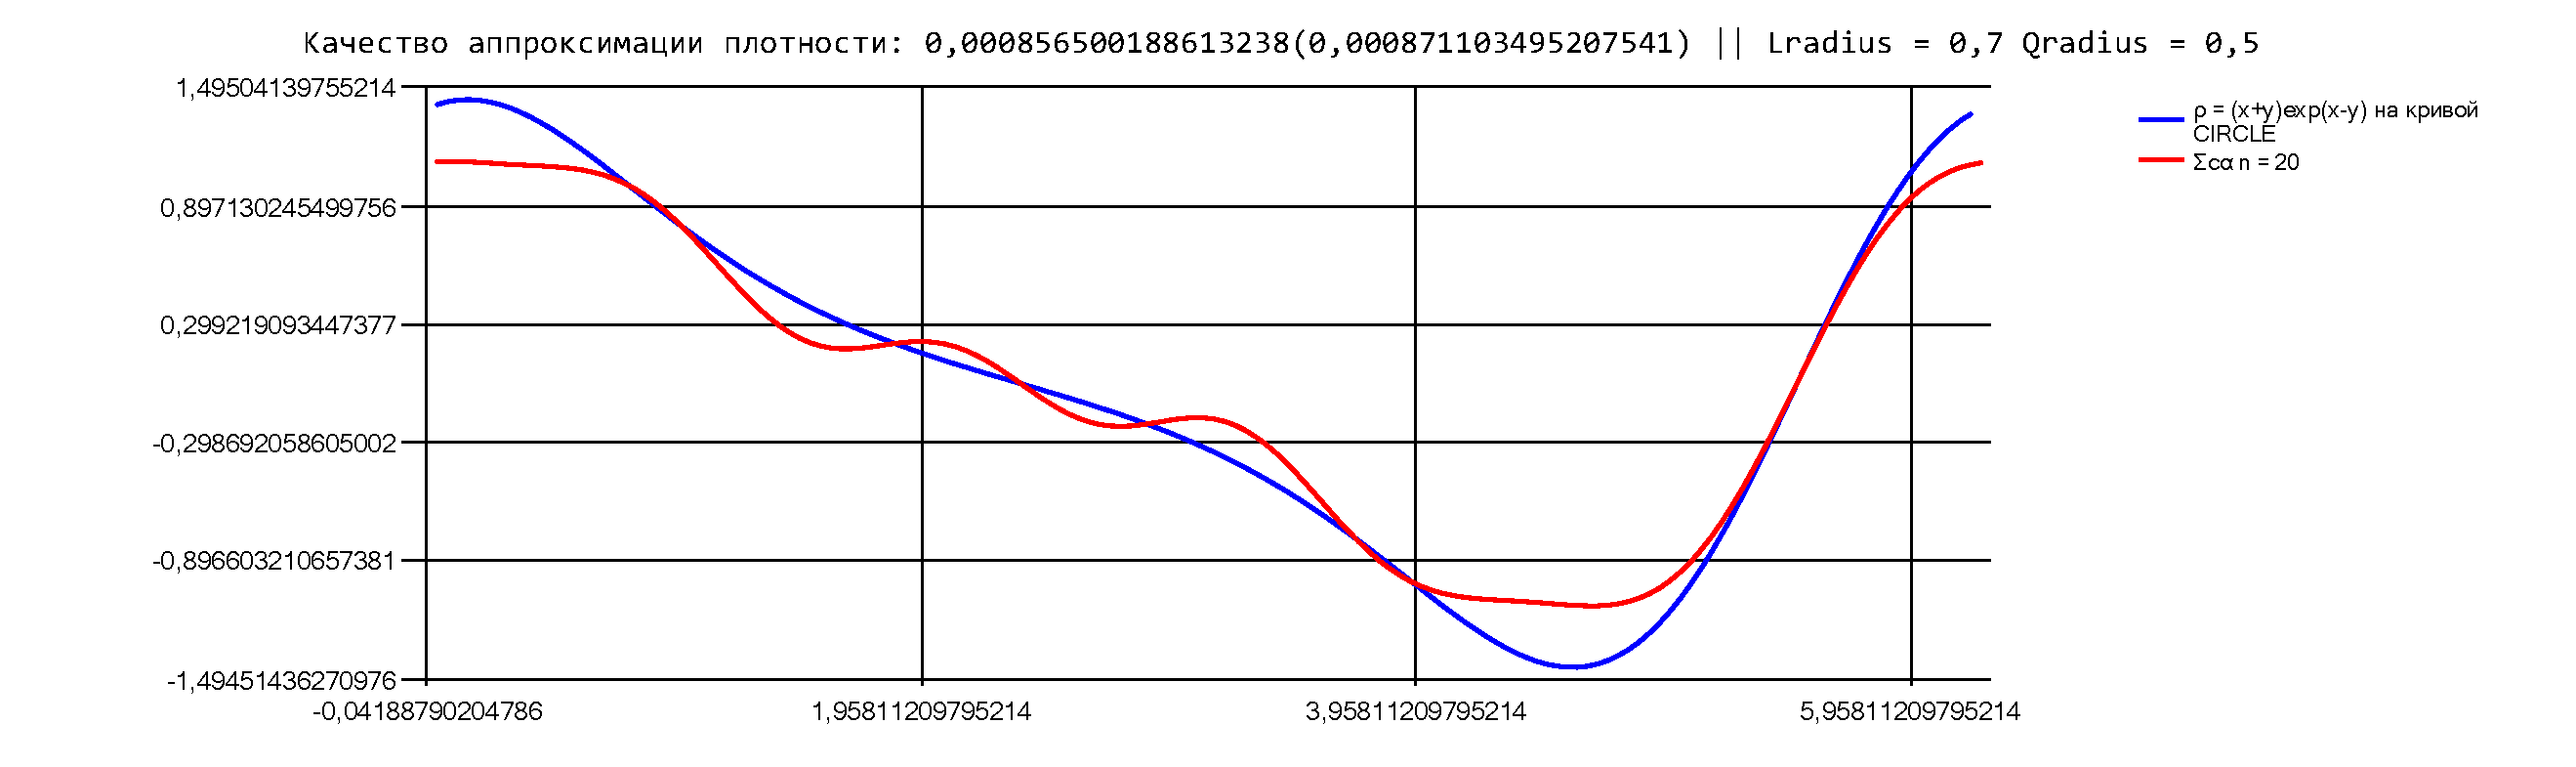
\includegraphics[width=0.8\linewidth]{d6.pdf} \\ для плотности} 
            \end{minipage}} 
            \vfill 
            \center{\begin{minipage}[h]{\linewidth} 
            \center{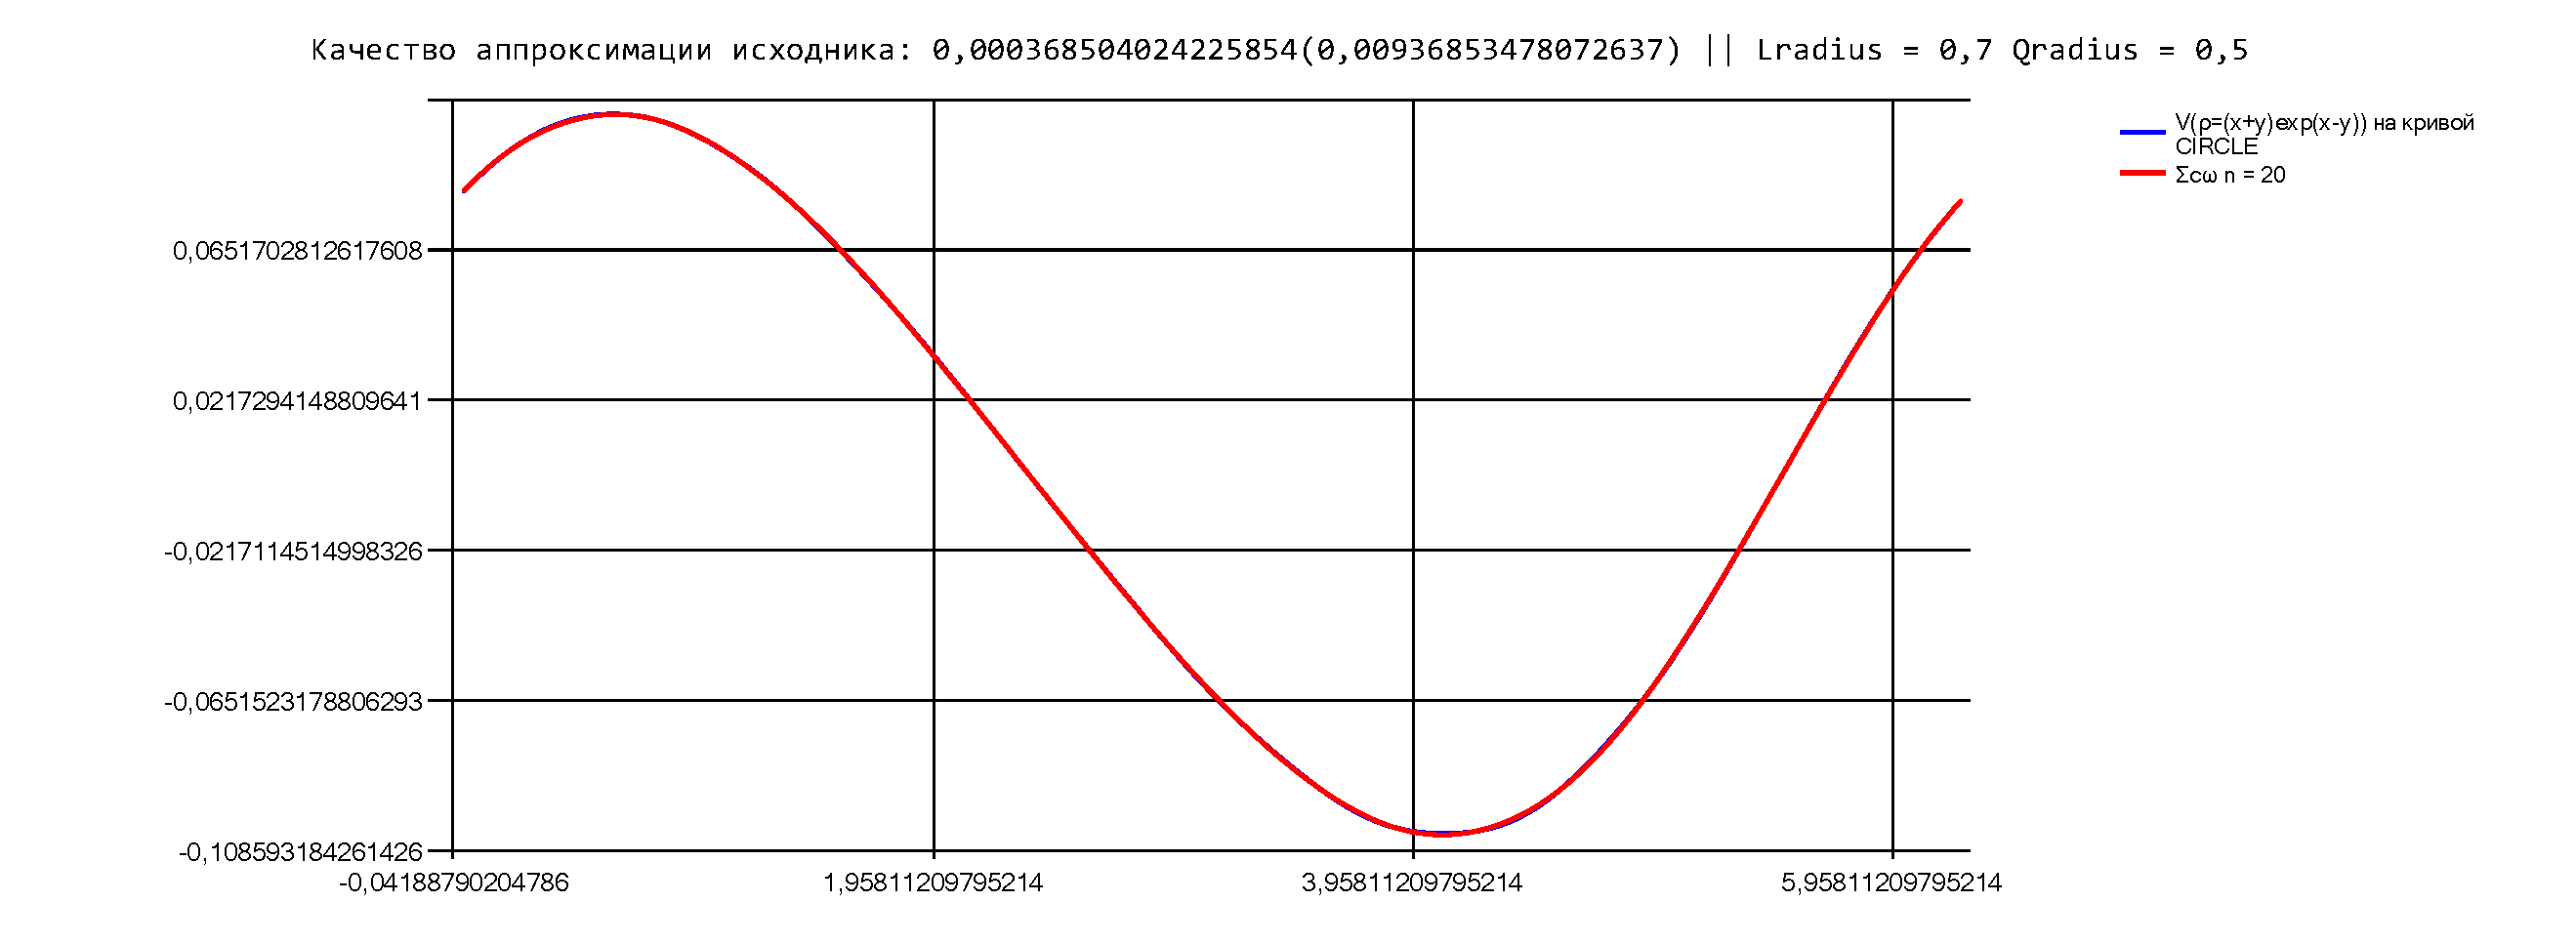
\includegraphics[width=0.8\linewidth]{v6.pdf} \\ для потенциала} 
            \end{minipage}} 
            \caption{Один из результатов работы алгоритма} 
            \label{ris:image1} 
            \end{figure}

            \begin{figure}[h] 
              \center{\begin{minipage}[h]{\linewidth} 
              \center{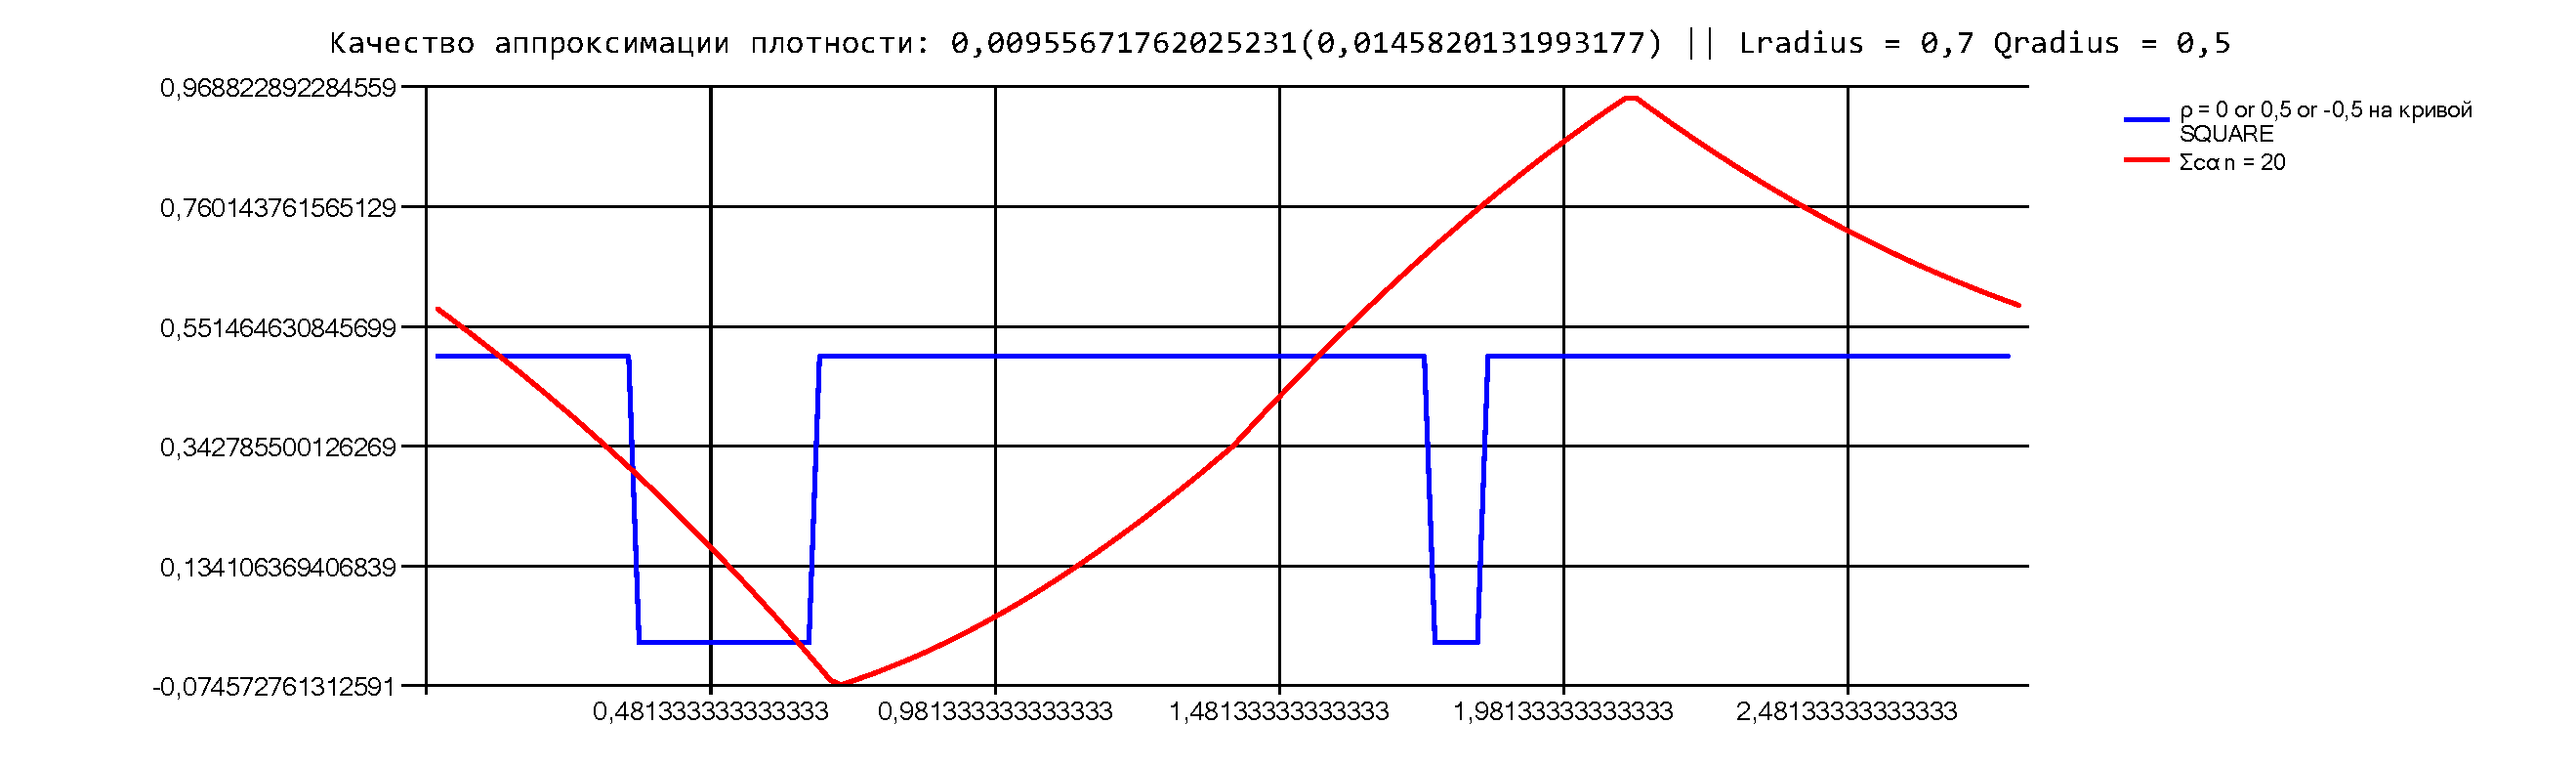
\includegraphics[width=0.8\linewidth]{d7.pdf} \\ для плотности} 
              \end{minipage}} 
              \vfill 
              \center{\begin{minipage}[h]{\linewidth} 
              \center{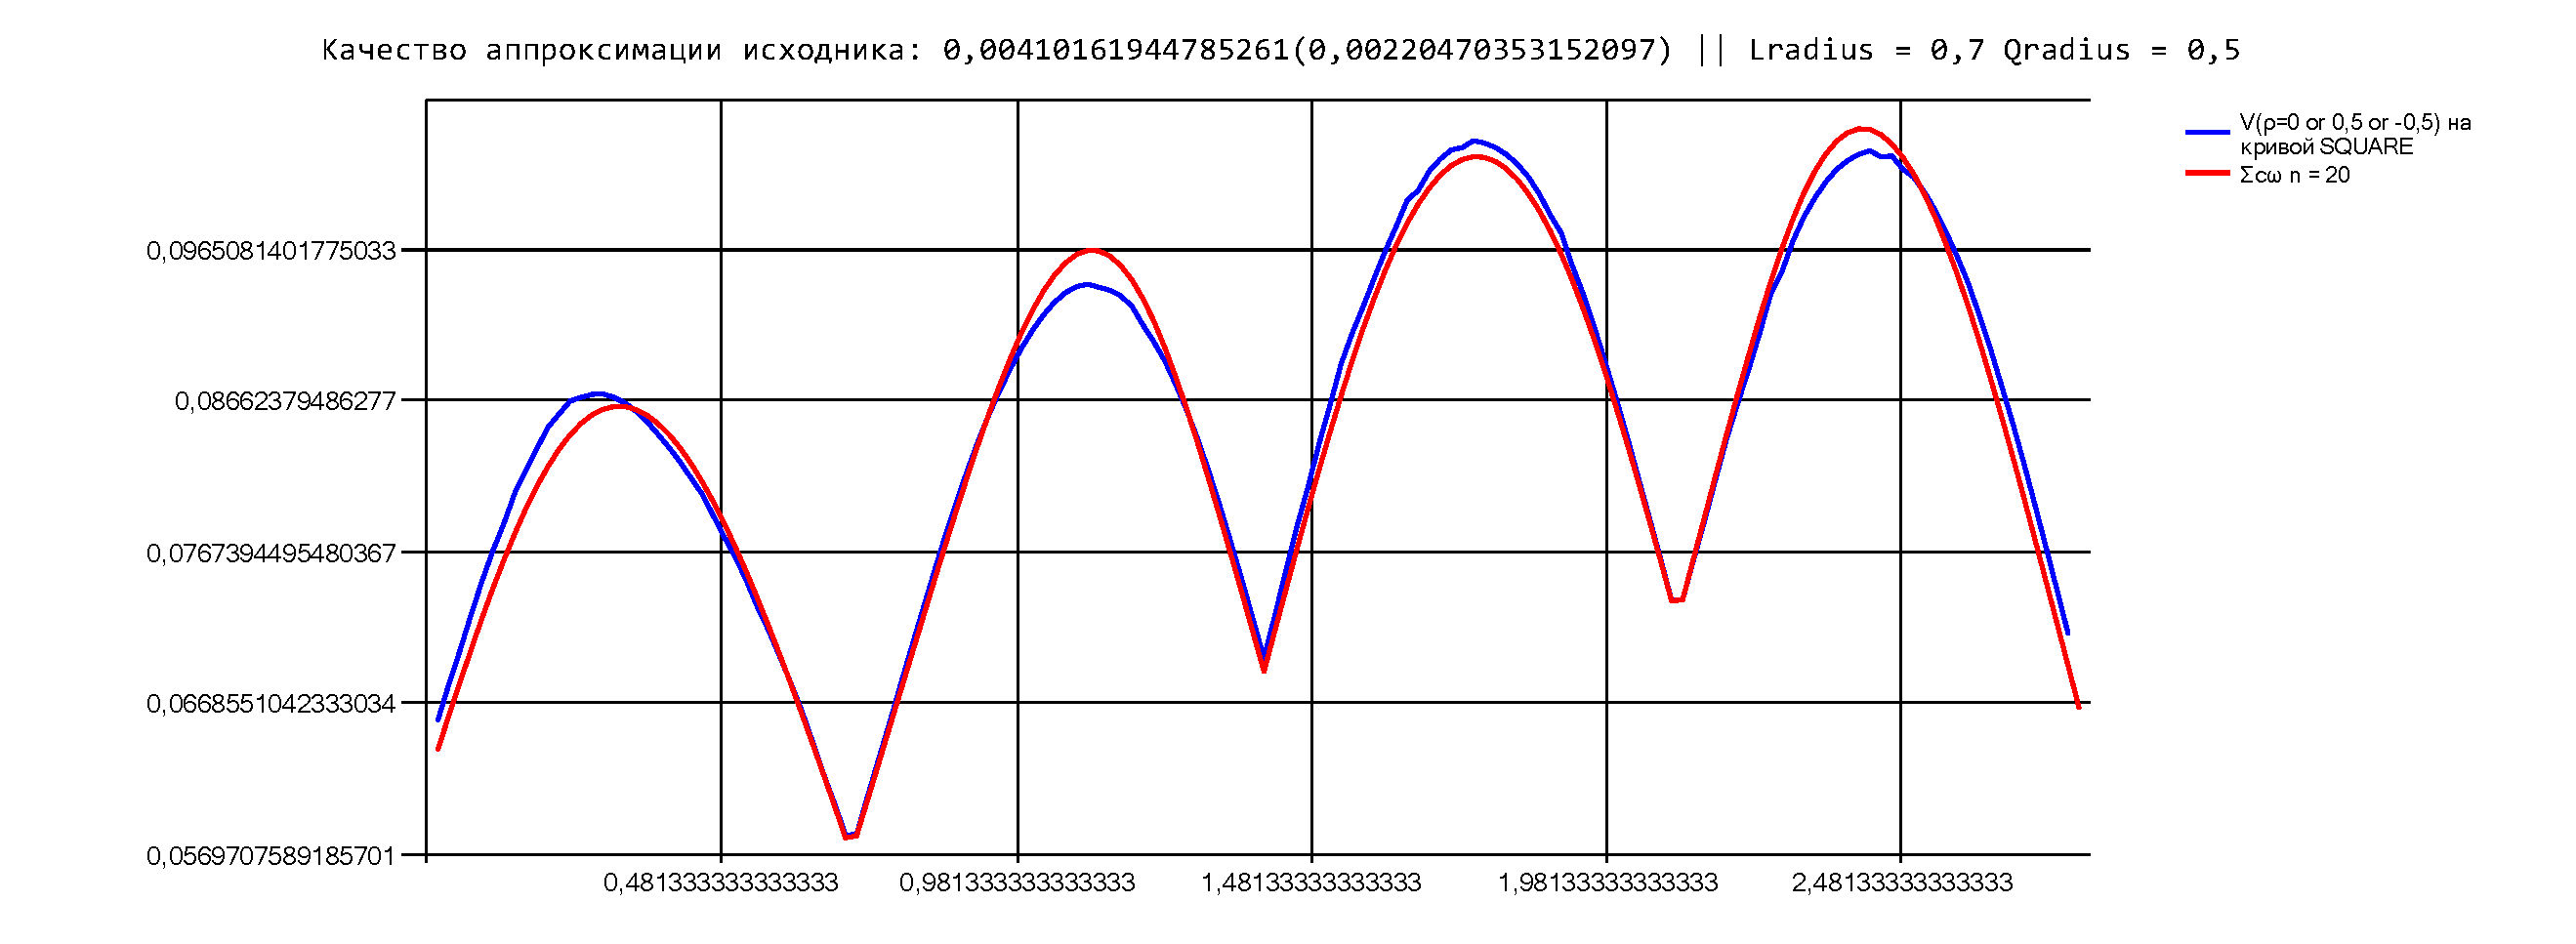
\includegraphics[width=0.8\linewidth]{v7.pdf} \\ для потенциала} 
              \end{minipage}} 
              \caption{Один из результатов работы алгоритма} 
              \label{p1} 
              \end{figure}

              \begin{figure}[h] 
                \center{\begin{minipage}[h]{\linewidth} 
                \center{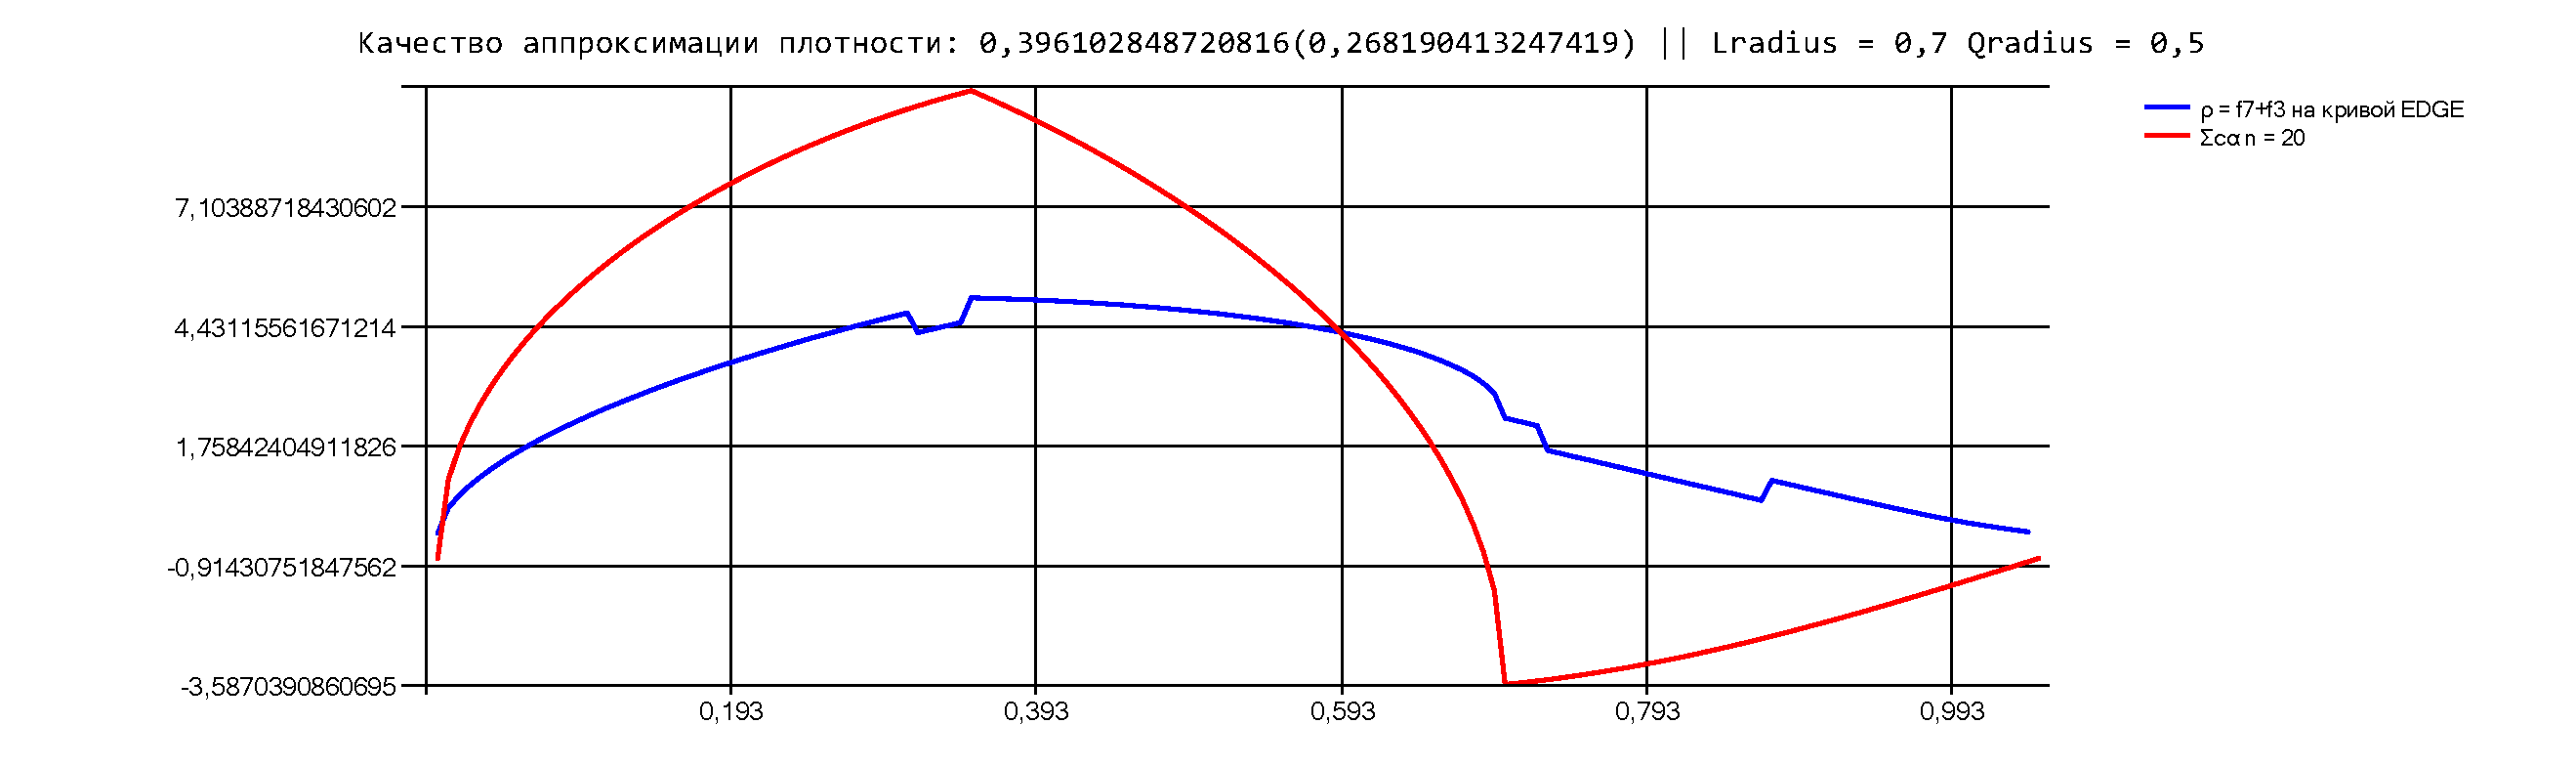
\includegraphics[width=0.8\linewidth]{d8.pdf} \\ для плотности} 
                \end{minipage}} 
                \vfill 
                \center{\begin{minipage}[h]{\linewidth} 
                \center{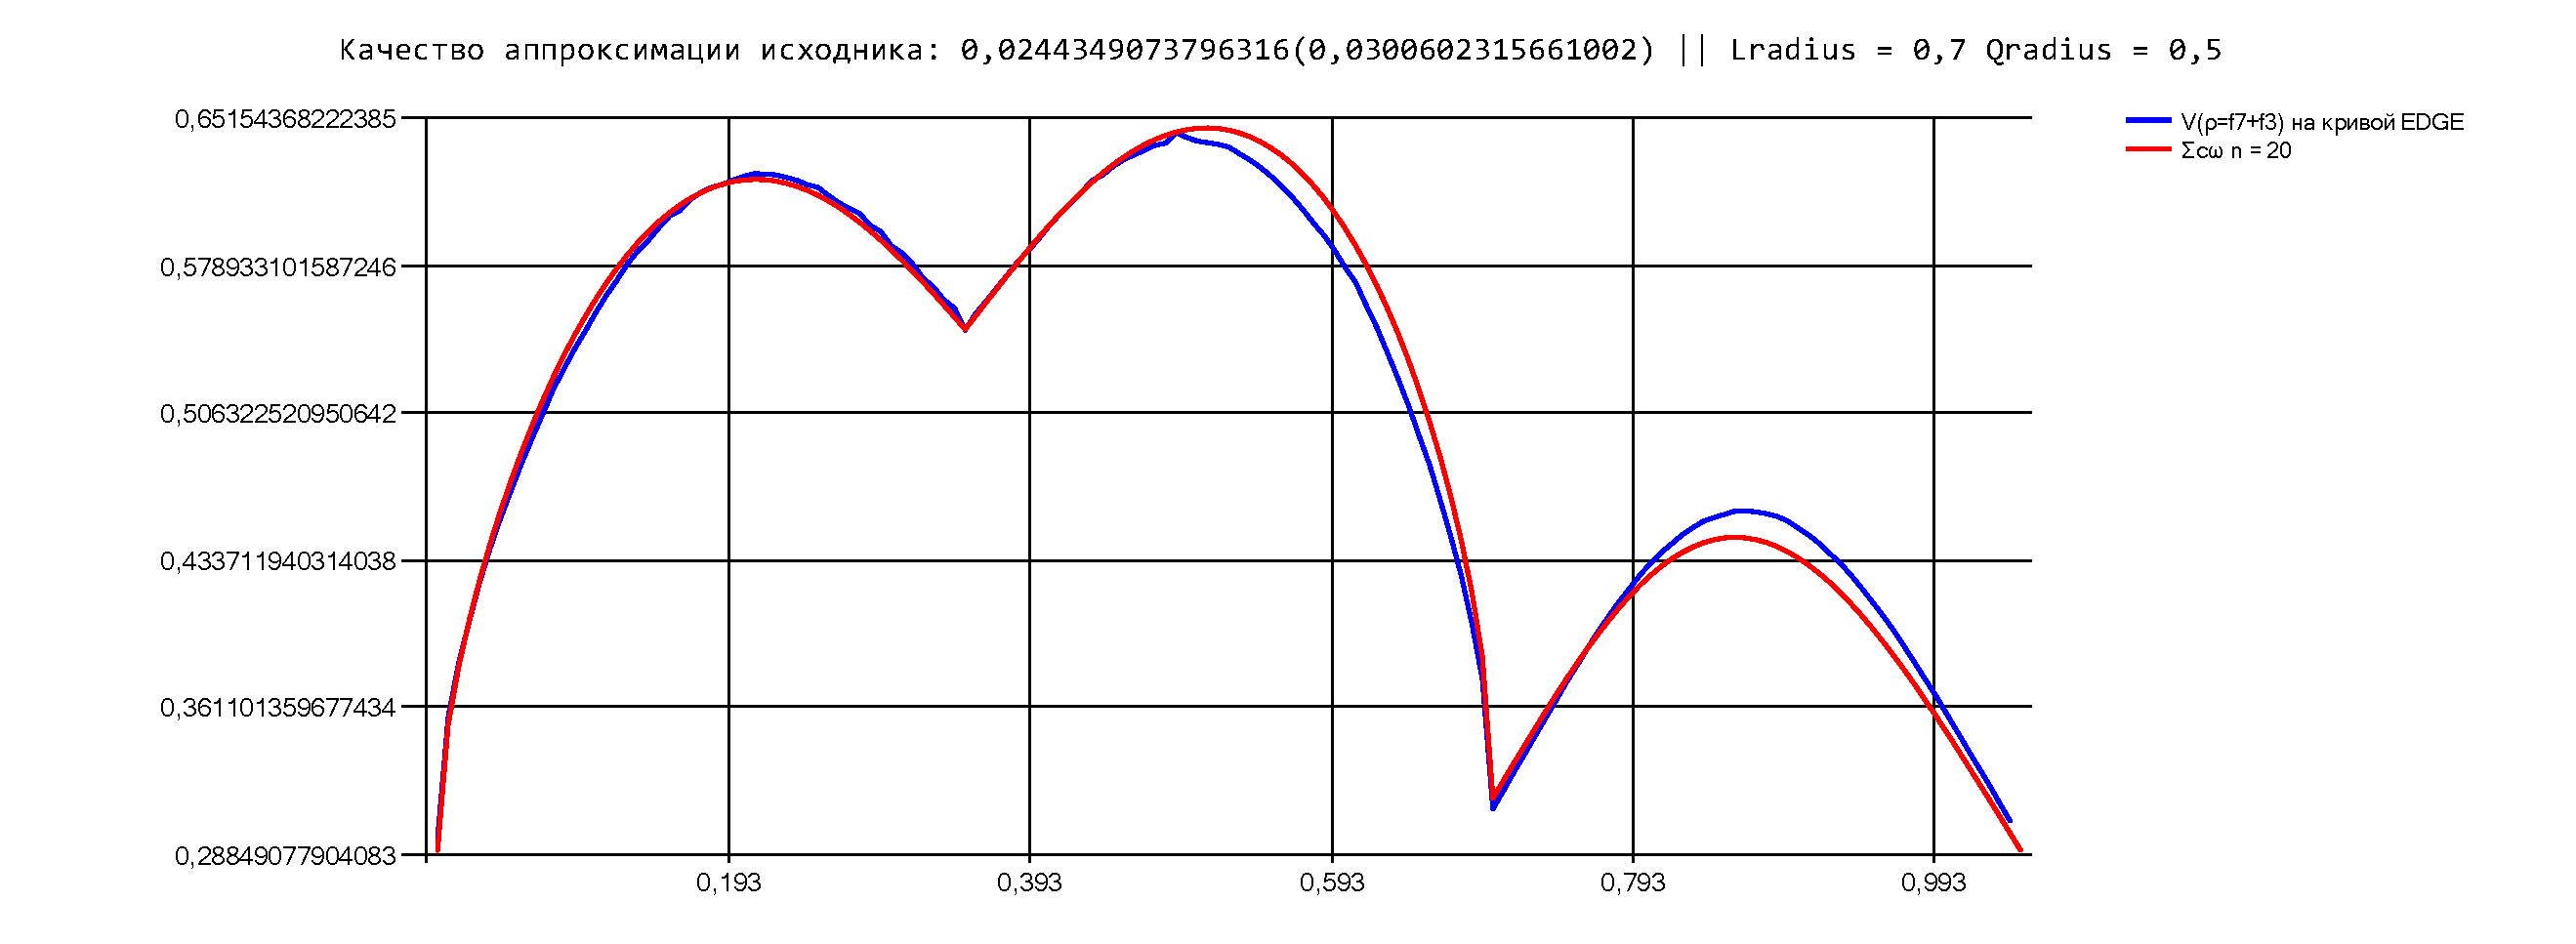
\includegraphics[width=0.8\linewidth]{v8.pdf} \\ для потенциала} 
                \end{minipage}} 
                \caption{Один из результатов работы алгоритма} 
                \label{p2} 
                \end{figure}


                \begin{figure}[h] 
                  \center{\begin{minipage}[h]{\linewidth} 
                  \center{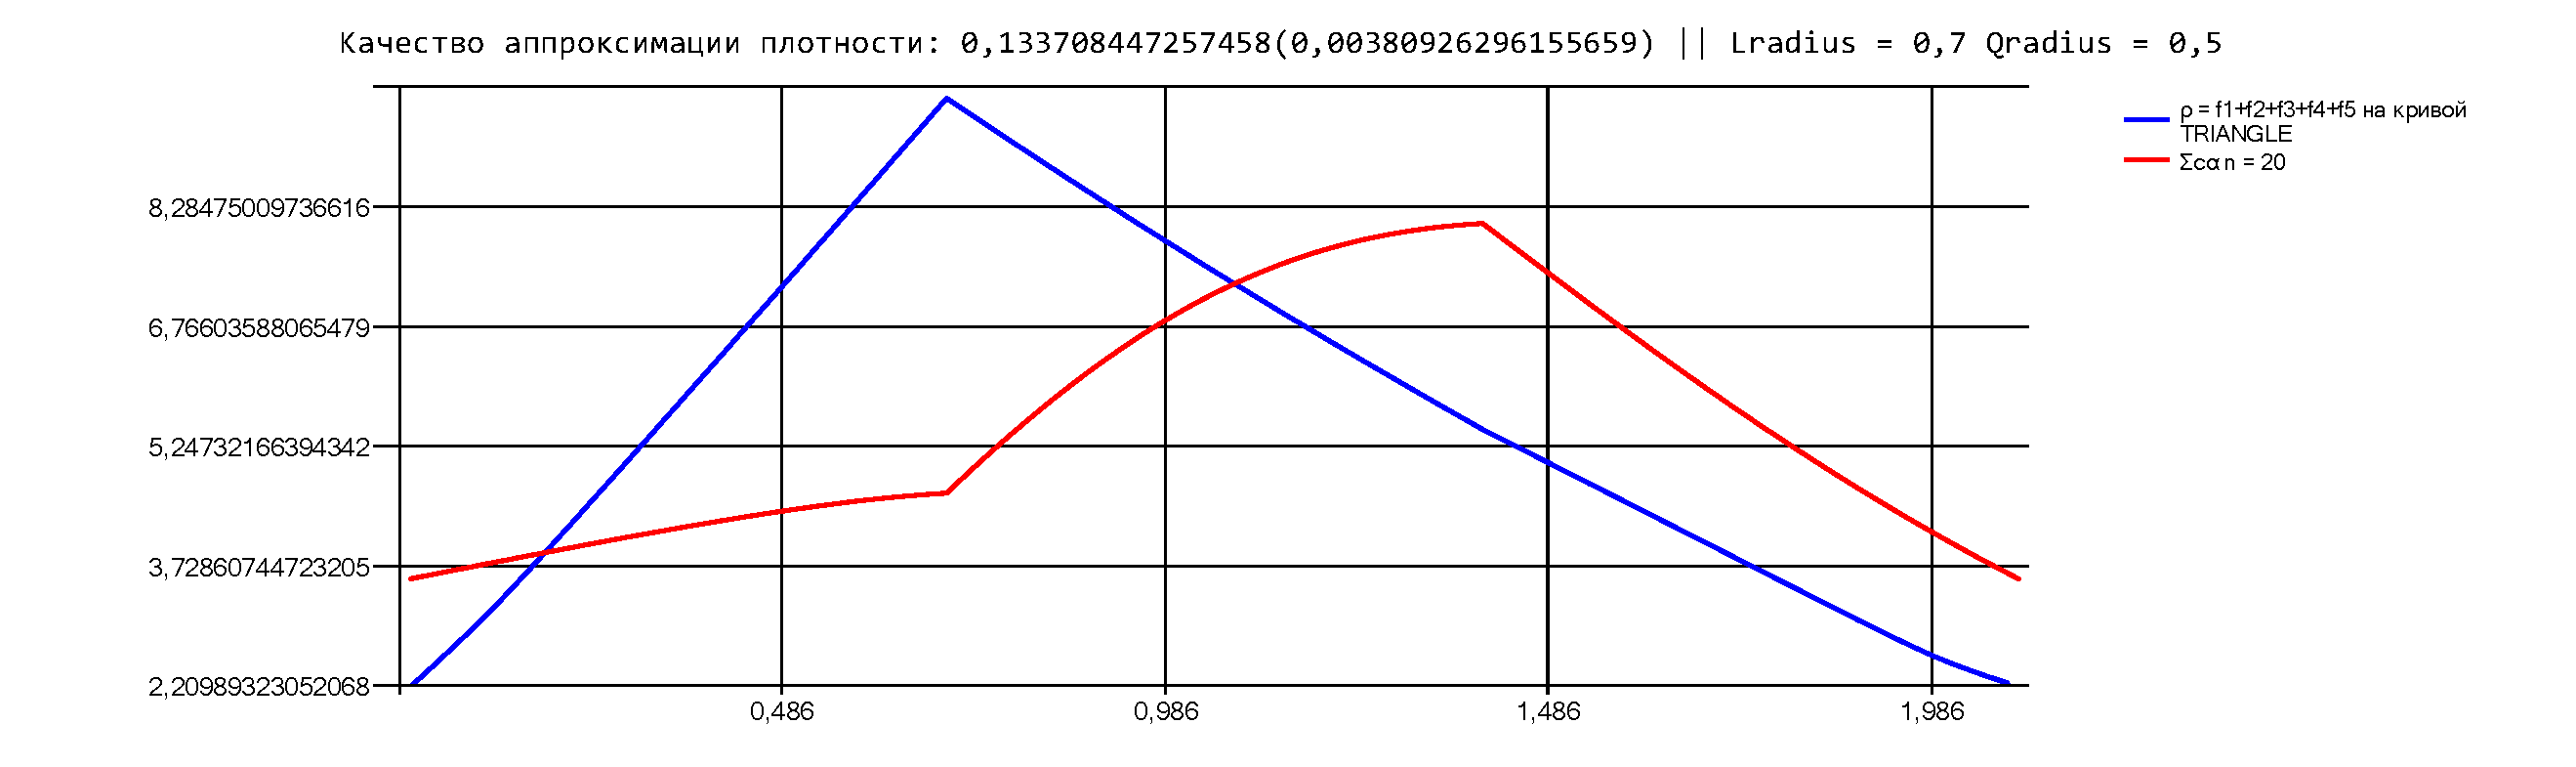
\includegraphics[width=0.8\linewidth]{d9.pdf} \\ для плотности} 
                  \end{minipage}} 
                  \vfill 
                  \center{\begin{minipage}[h]{\linewidth} 
                  \center{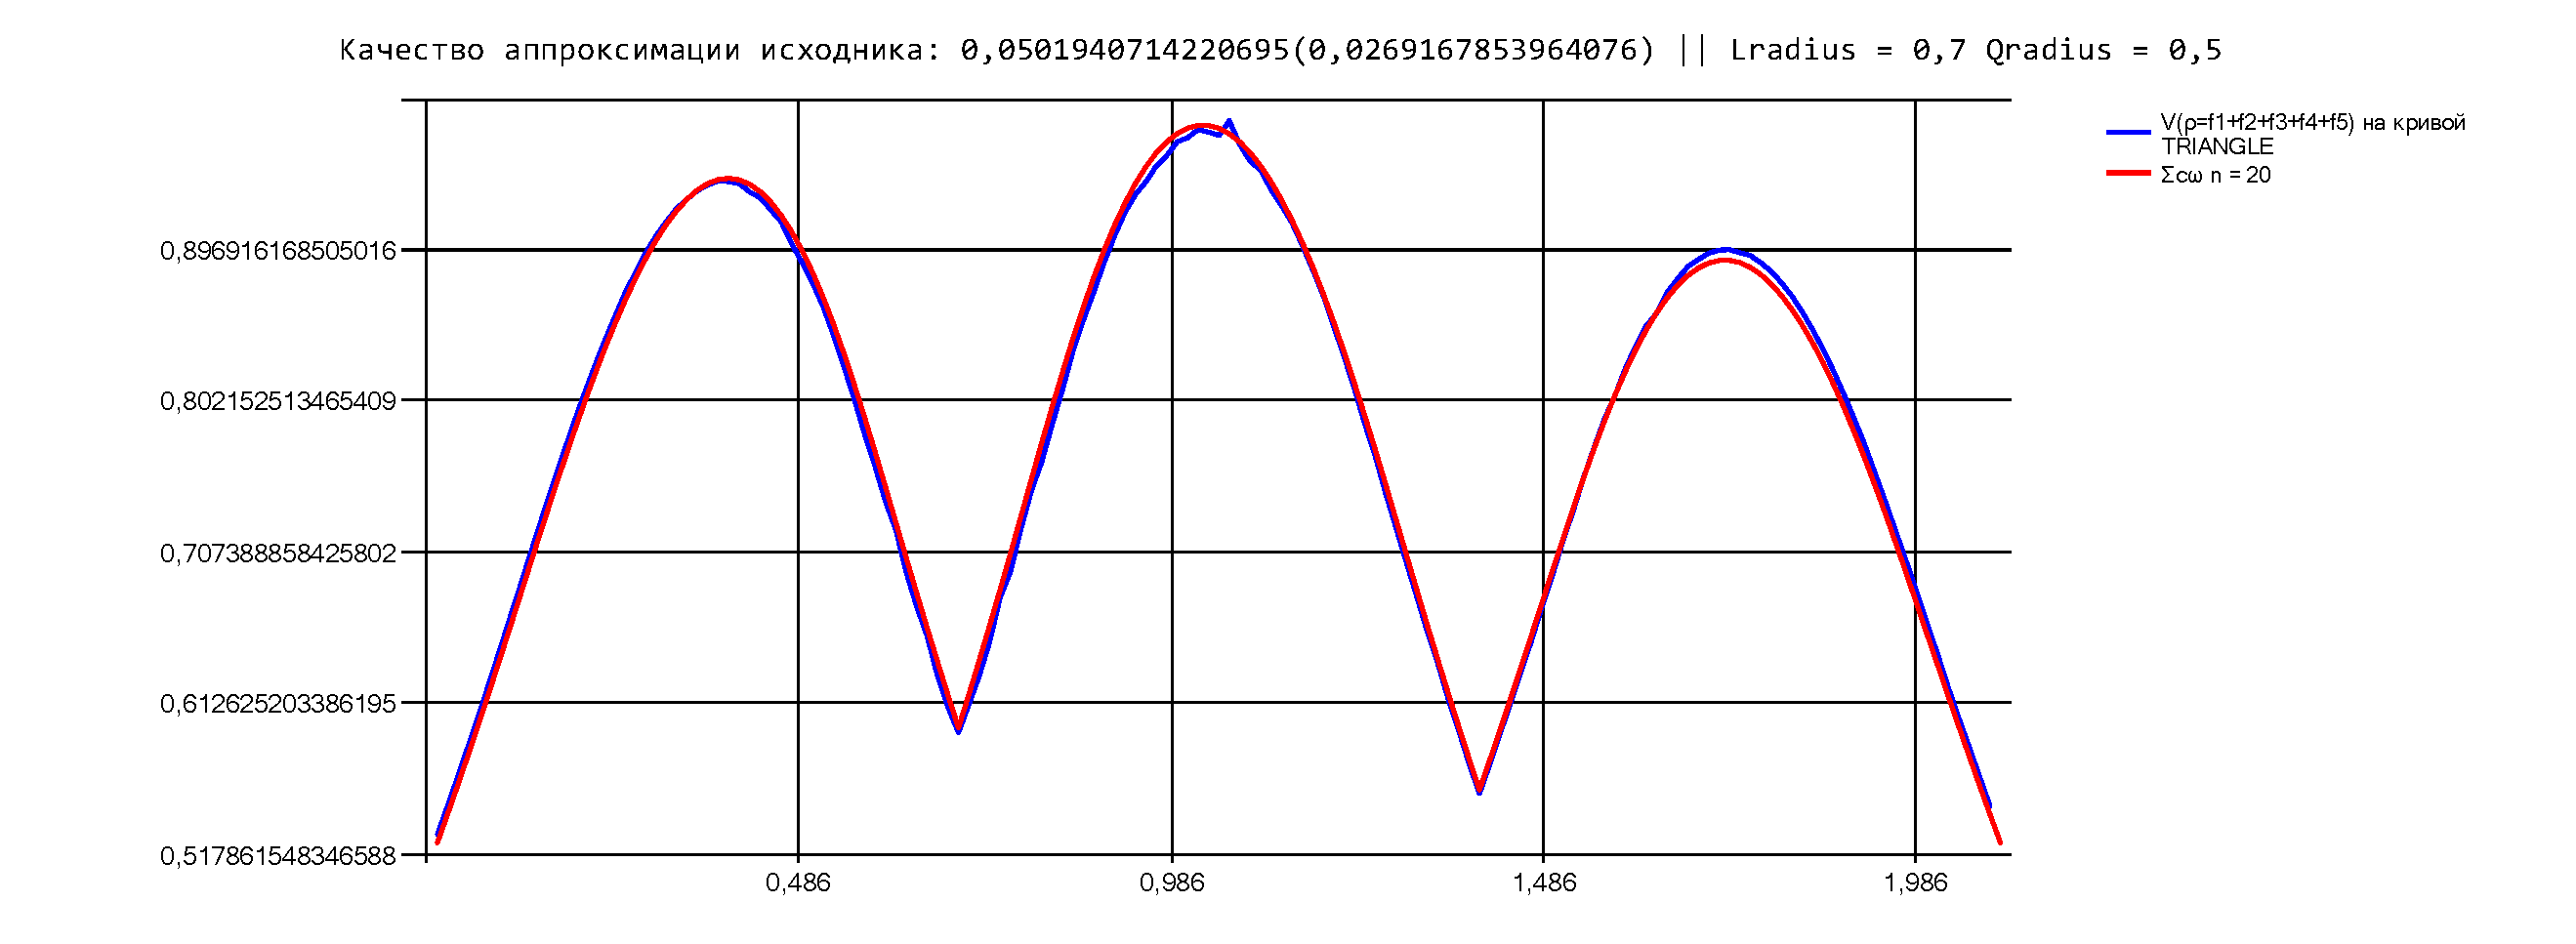
\includegraphics[width=0.8\linewidth]{v9.pdf} \\ для потенциала} 
                  \end{minipage}} 
                  \caption{Один из результатов работы алгоритма} 
                  \label{ris:image1} 
                  \end{figure}

                  \begin{figure}[h] 
                    \center{\begin{minipage}[h]{\linewidth} 
                    \center{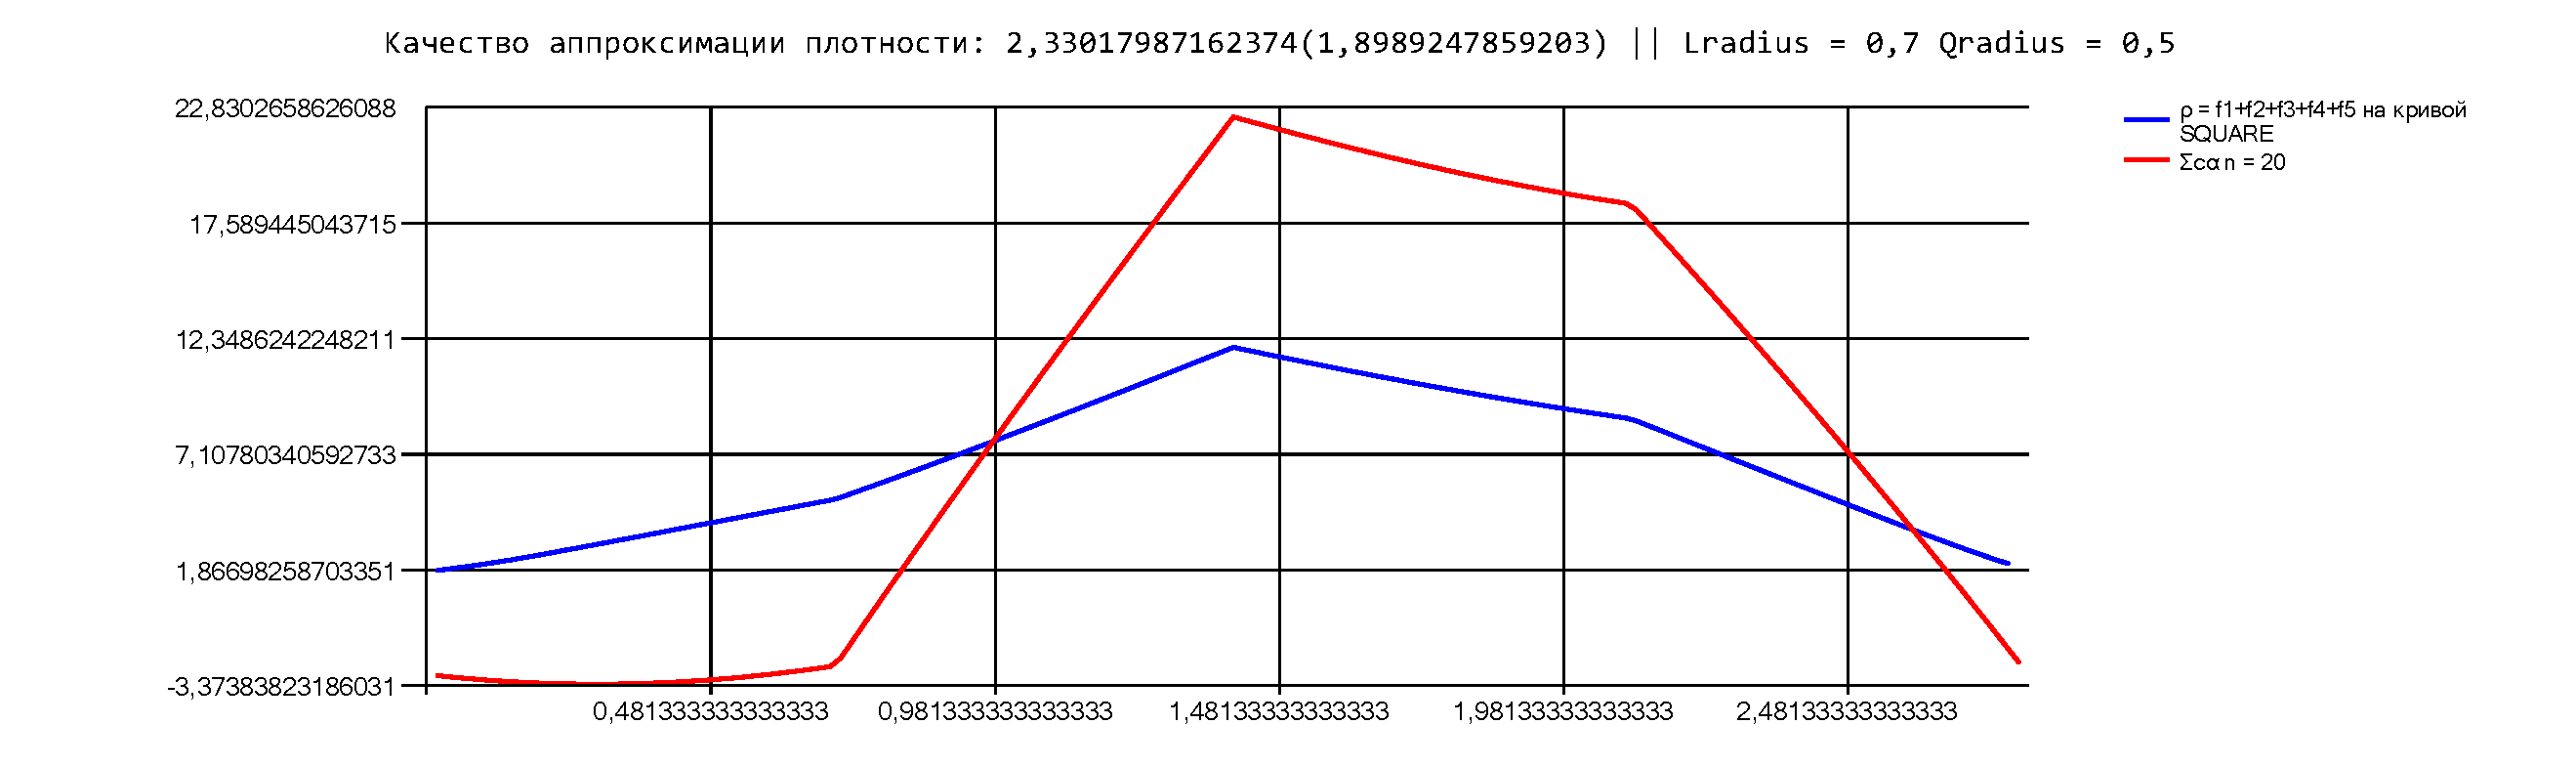
\includegraphics[width=0.8\linewidth]{d10.pdf} \\ для плотности} 
                    \end{minipage}} 
                    \vfill 
                    \center{\begin{minipage}[h]{\linewidth} 
                    \center{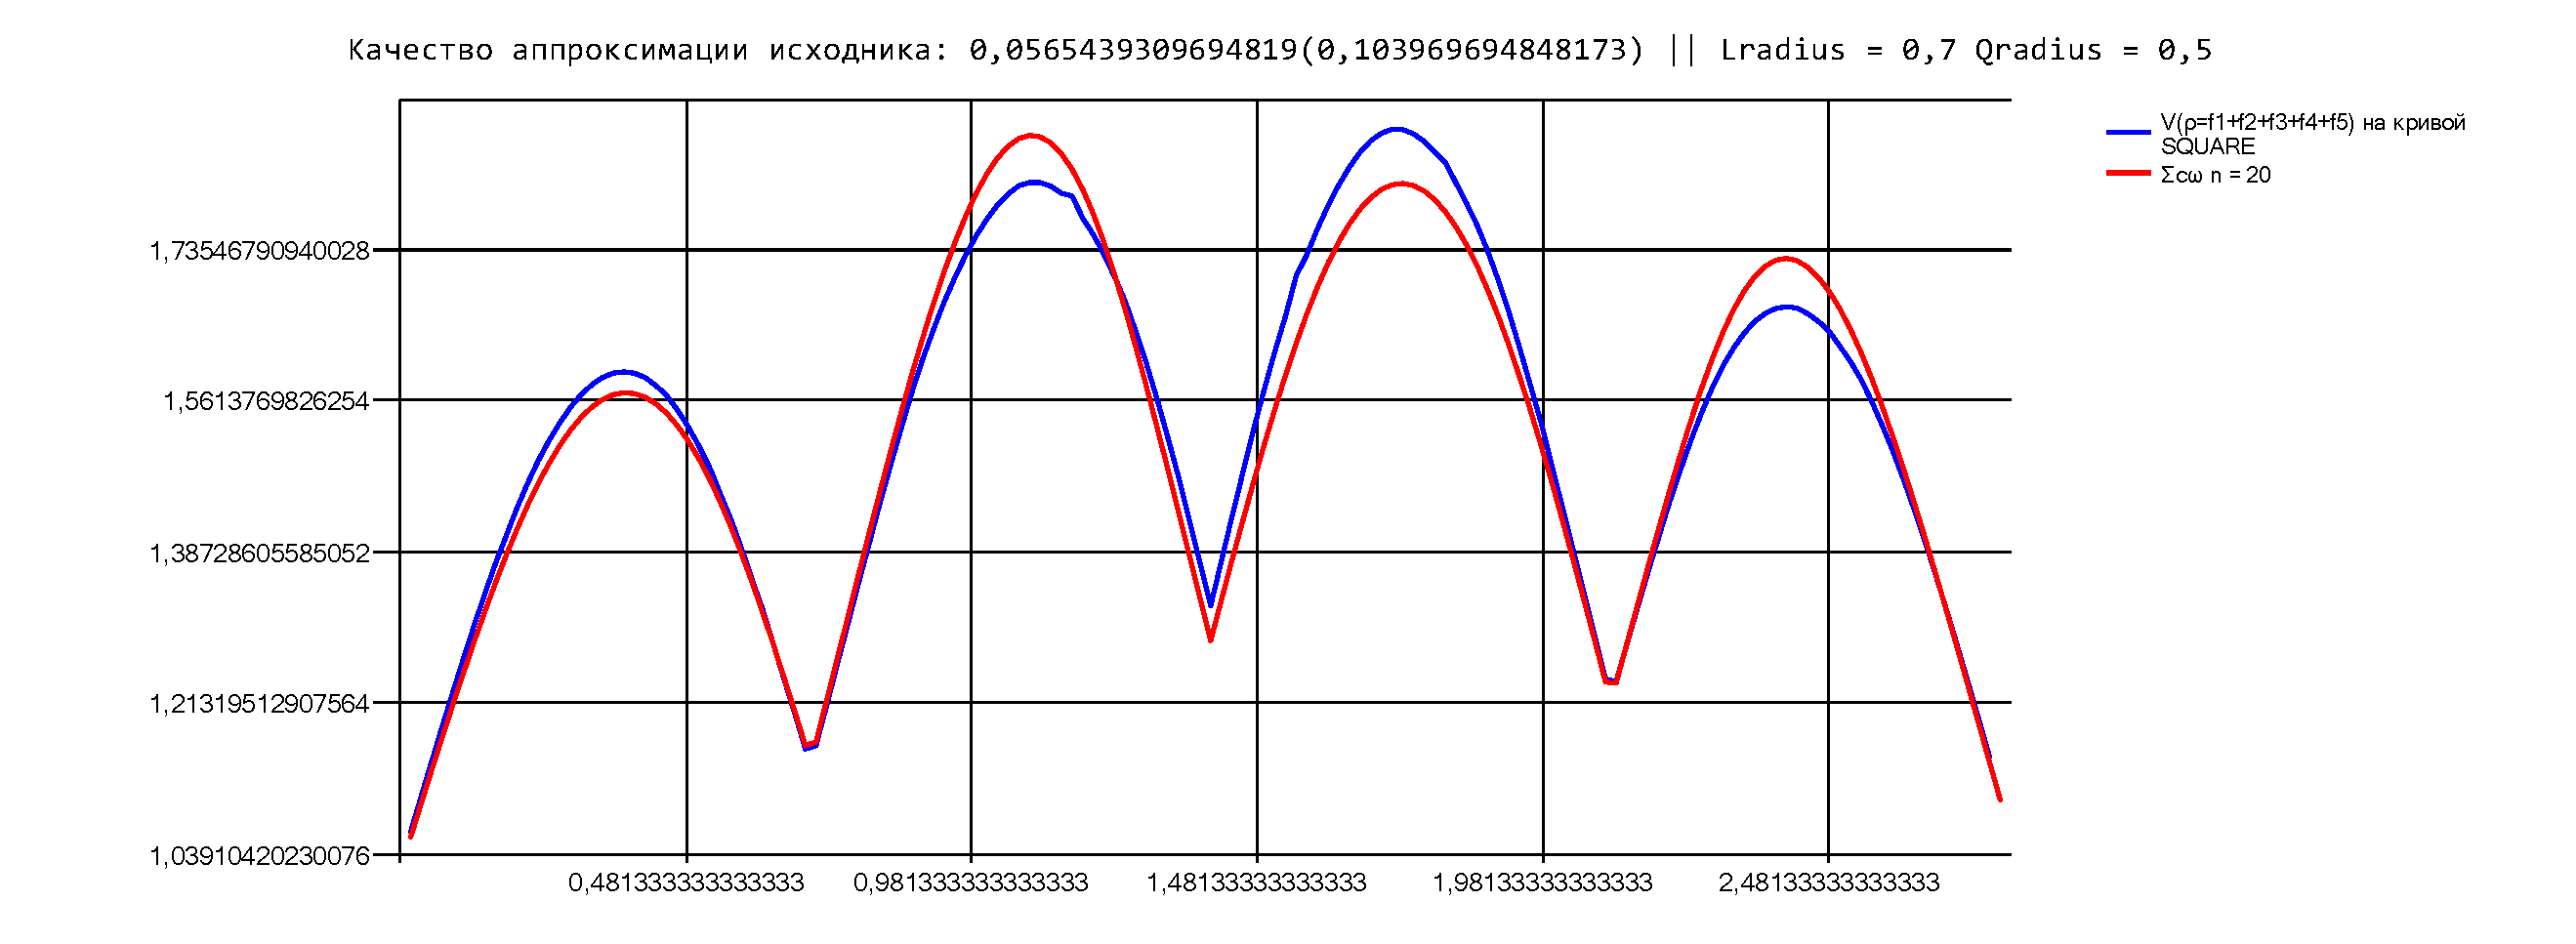
\includegraphics[width=0.8\linewidth]{v10.pdf} \\ для потенциала} 
                    \end{minipage}} 
                    \caption{Один из результатов работы алгоритма} 
                    \label{hexampl} 
                    \end{figure}                                        

Рассмотрев результаты тестирования (несколько сотен графиков), я сделал вывод, что в среднем аппроксимация по круговой области происходит немного лучше.
%Для других областей, возможно, требует увеличивать точность интегрирования, либо сам характер области оказывает влияние на работу метода (на рисунке \ref{hexampl} показана аппроксимация первого базисного потенциала на треугольнике, которая логически должна составлял абсолютный ноль).
Однако, некоторые функции лучше аппроксимировались на некруговых областях.
Кроме этого, хорошая аппроксимация $||V_f-V_{\tilde{\rho} } ||_{L_2(L)}$ не всегда означает хорошую аппроксимацию $||\rho-\tilde{\rho} ||_{L_2(Q)}$ (неустойчивость заметна на многих рисунках).%, рисунки \ref{p1},\ref{p2},\ref{p3},\ref{p4},\ref{p5},\ref{p6},\ref{p7}).

\subsection{3D-графики}
Если 2D-графики из прошлого подраздела показывали особенности аппроксимации на границе области $Q$, то следующие графики показывают поведение погрешности по всей области в целом.
В следующих графиках (рисунки \ref{d3beg}-\ref{d3end}) число базисных потенциалов равно $20$, под Density имеется в виду плотность $\rho$, под Density approx. --- $\tilde{\rho}$, под Difference --- функция $|\rho-\tilde{\rho}|$.

\begin{figure}[h]
  \begin{minipage}[h]{0.49\linewidth}
  \center{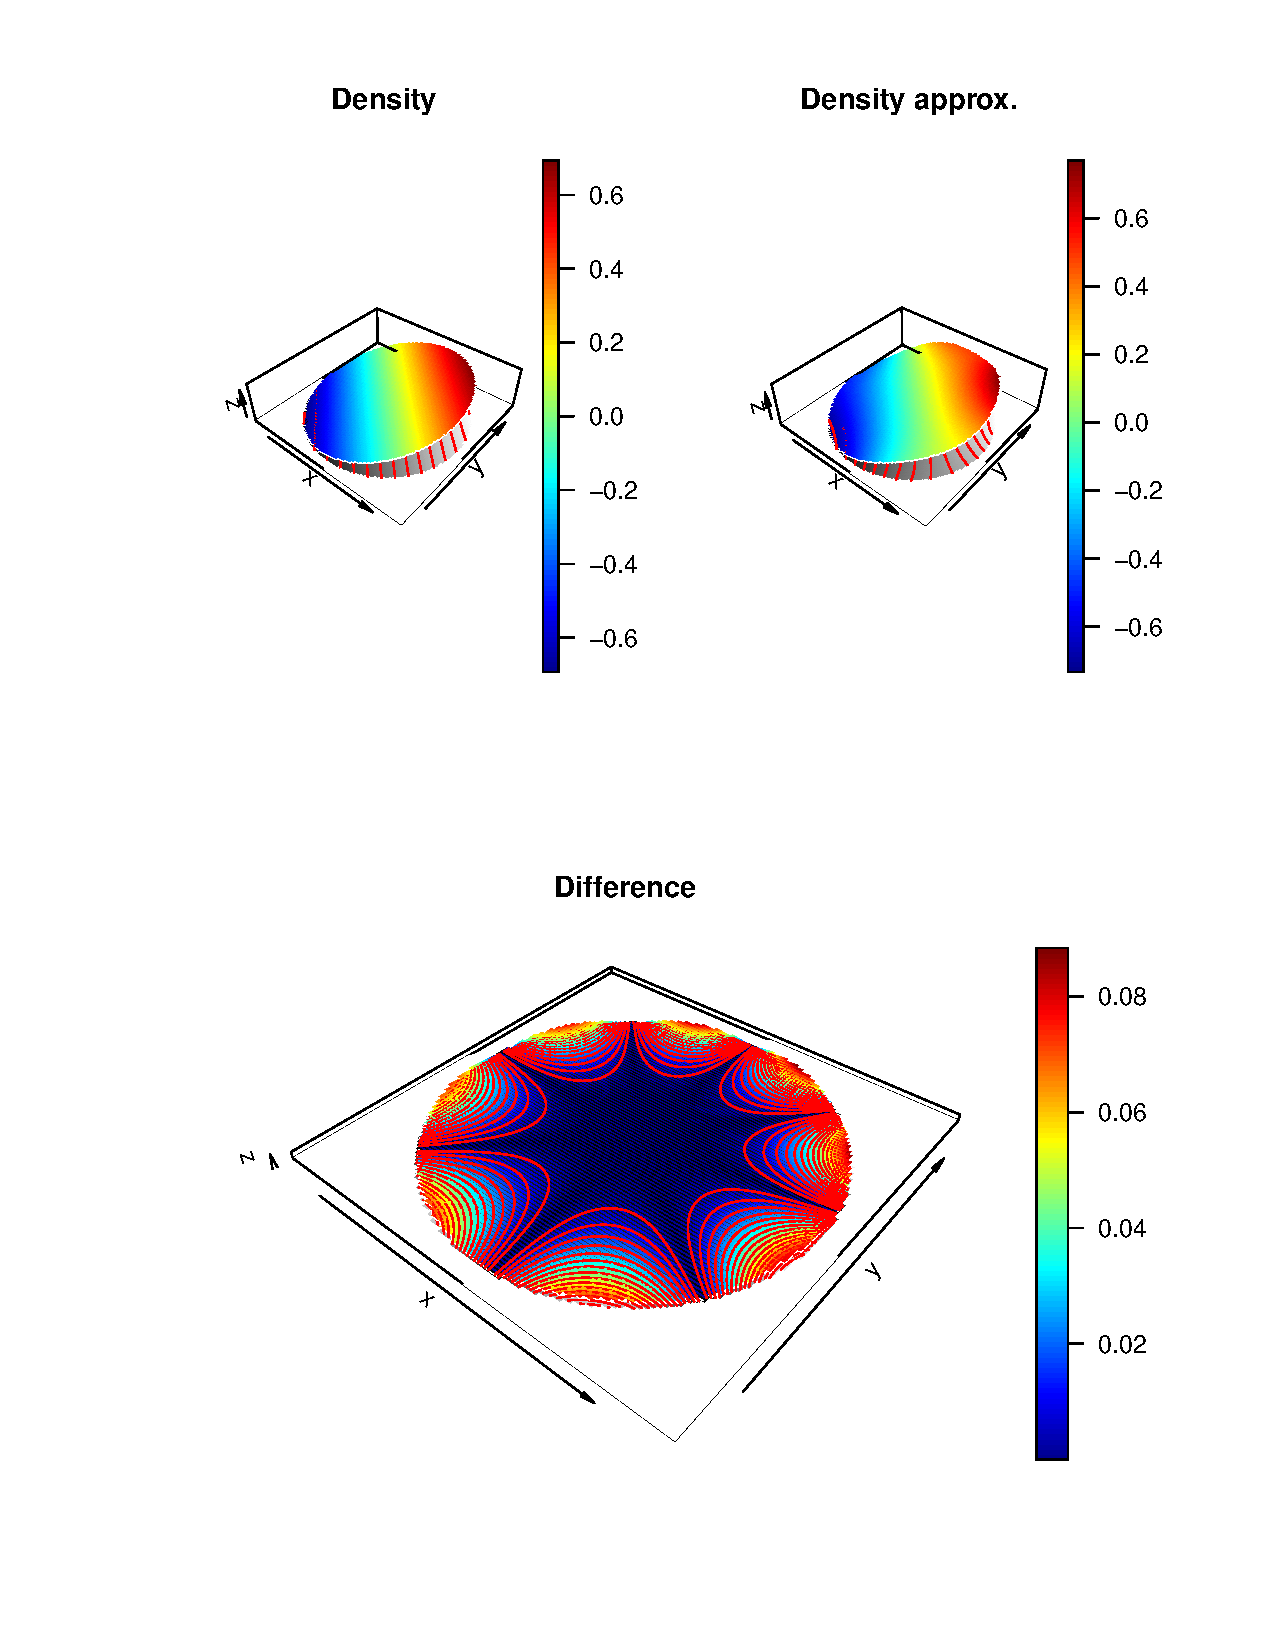
\includegraphics[width=0.95\linewidth]{f11.pdf}}
  \end{minipage}
  \hfill
  \begin{minipage}[h]{0.49\linewidth}
  \center{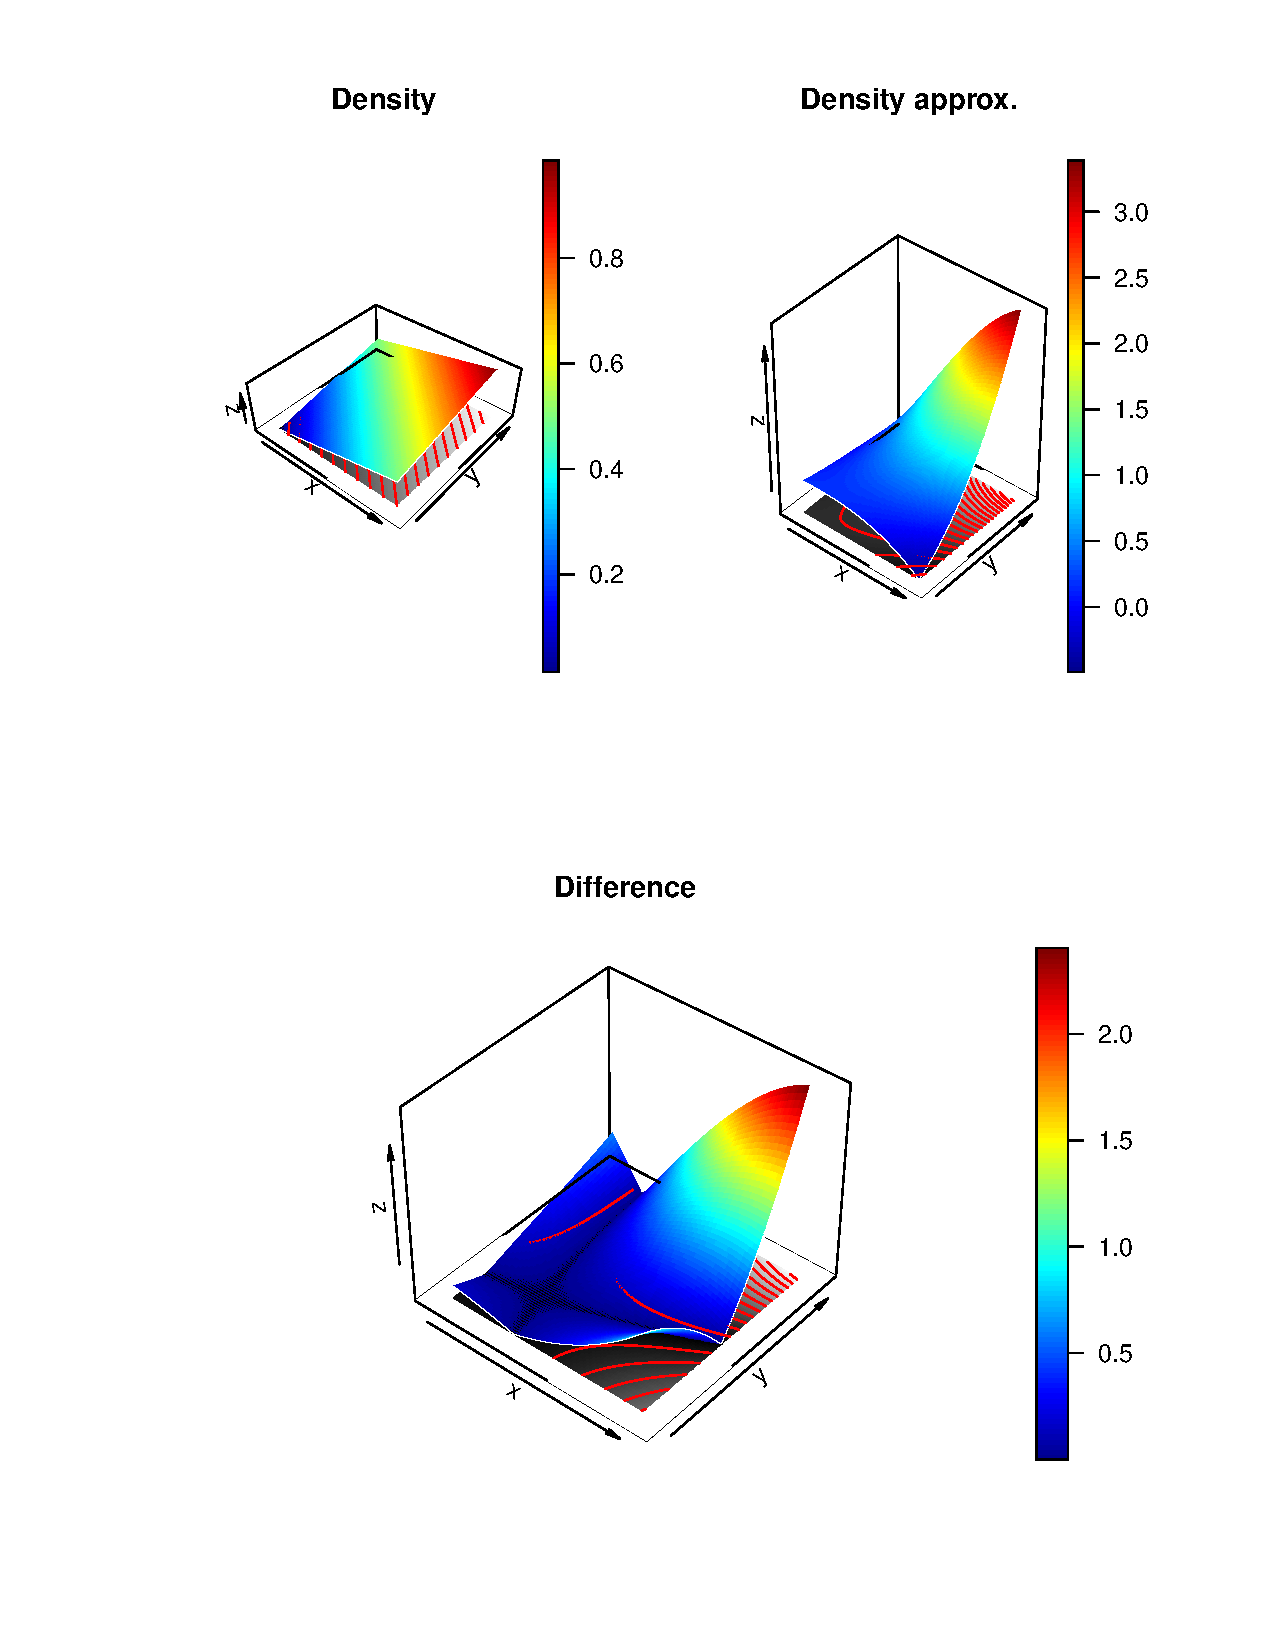
\includegraphics[width=0.95\linewidth]{f13.pdf}}
  \end{minipage}
  \caption{Для $f_1$}
  \label{d3beg}
  \end{figure}

  \begin{figure}[h]
    \begin{minipage}[h]{0.49\linewidth}
    \center{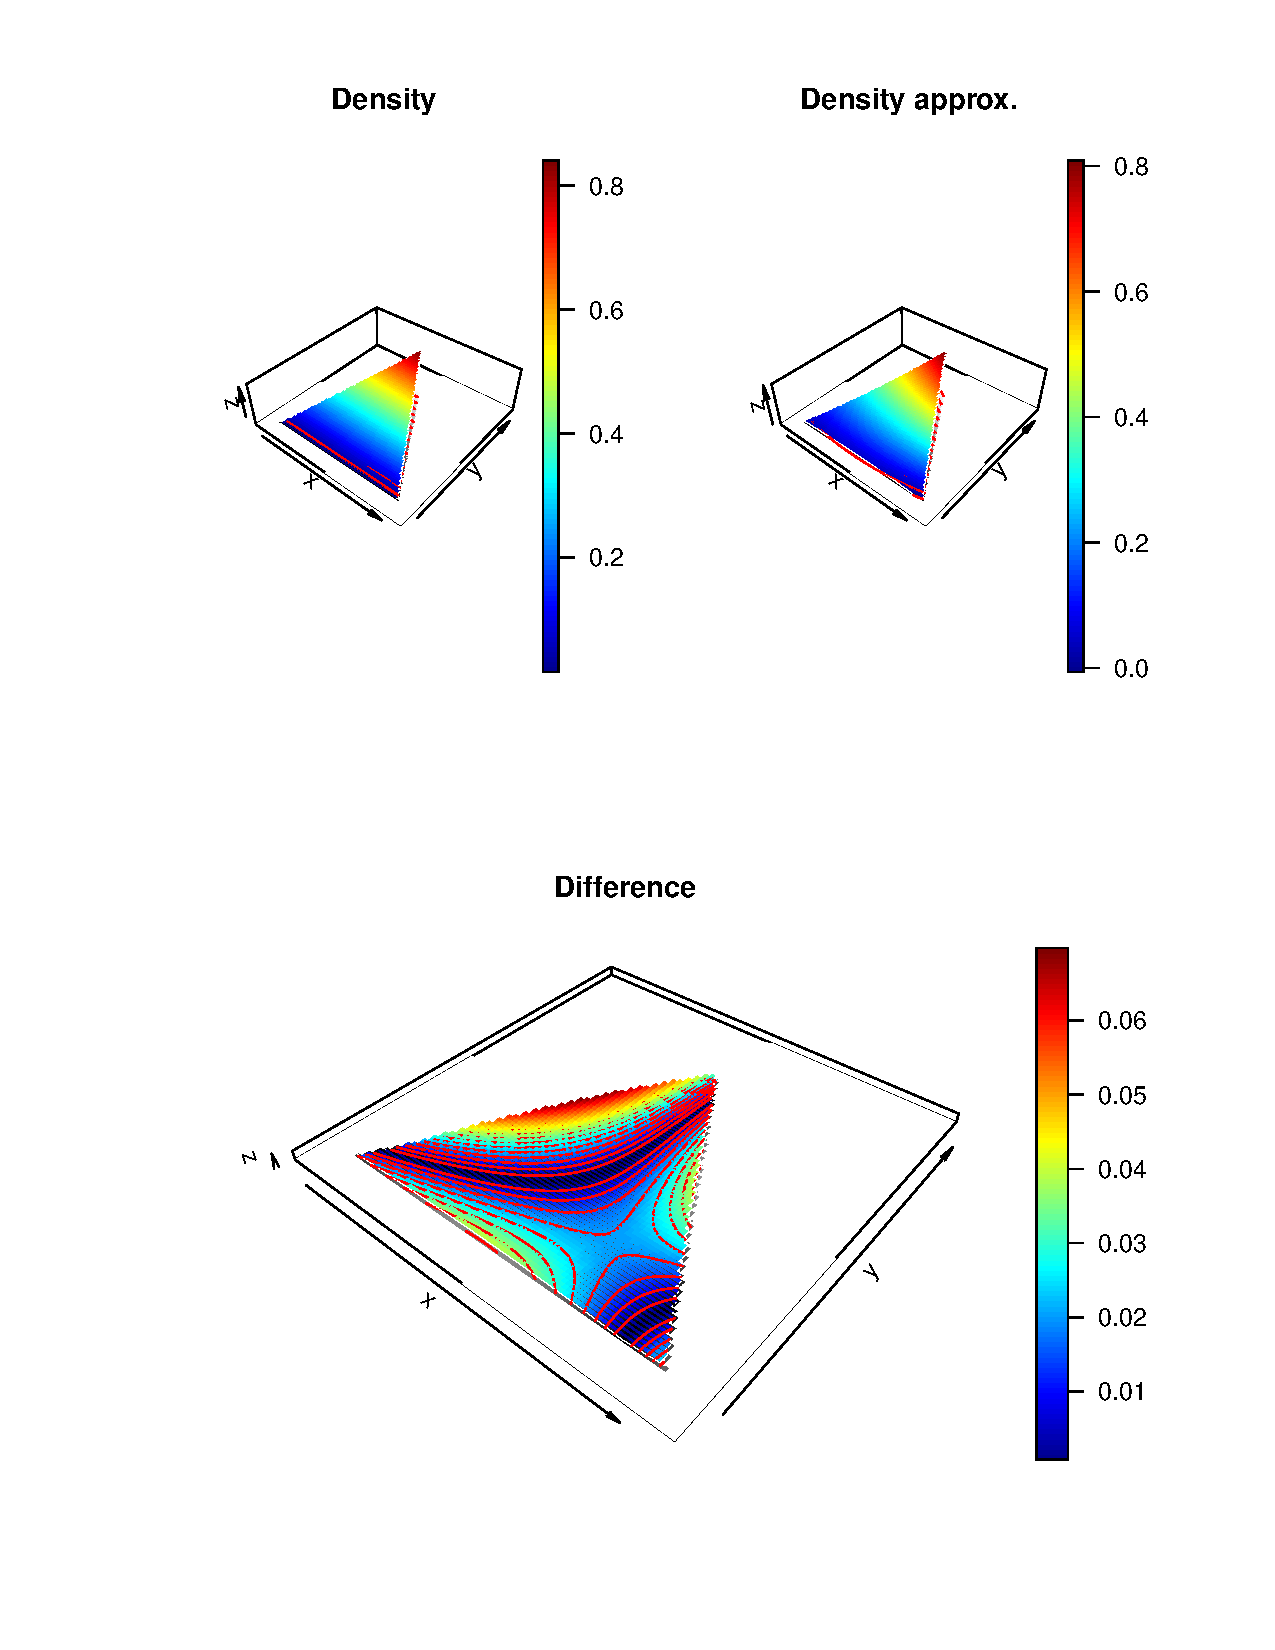
\includegraphics[width=0.95\linewidth]{f22.pdf}}
    \end{minipage}
    \hfill
    \begin{minipage}[h]{0.49\linewidth}
    \center{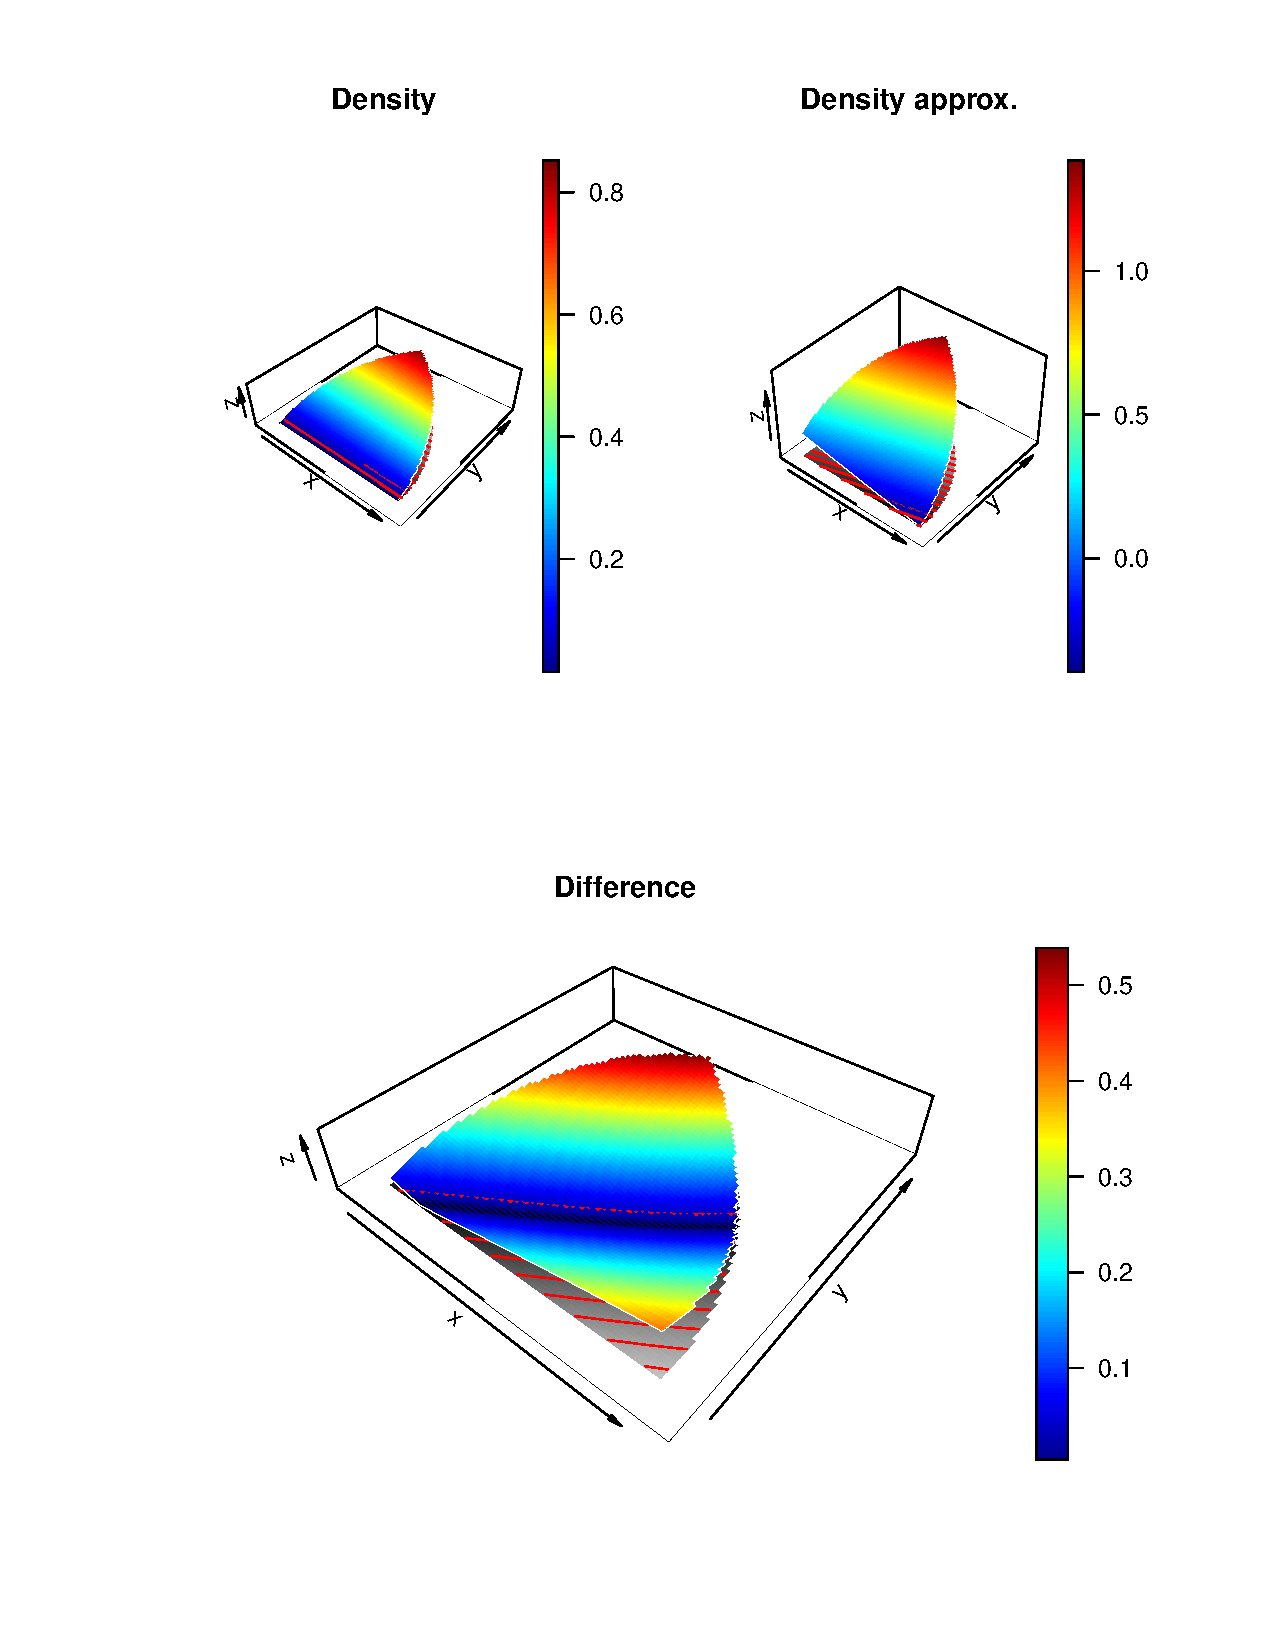
\includegraphics[width=0.95\linewidth]{f24.pdf}}
    \end{minipage}
    \caption{Для $f_2$}
    \label{ris:image1}
    \end{figure}

    \begin{figure}[h]
      \begin{minipage}[h]{0.49\linewidth}
      \center{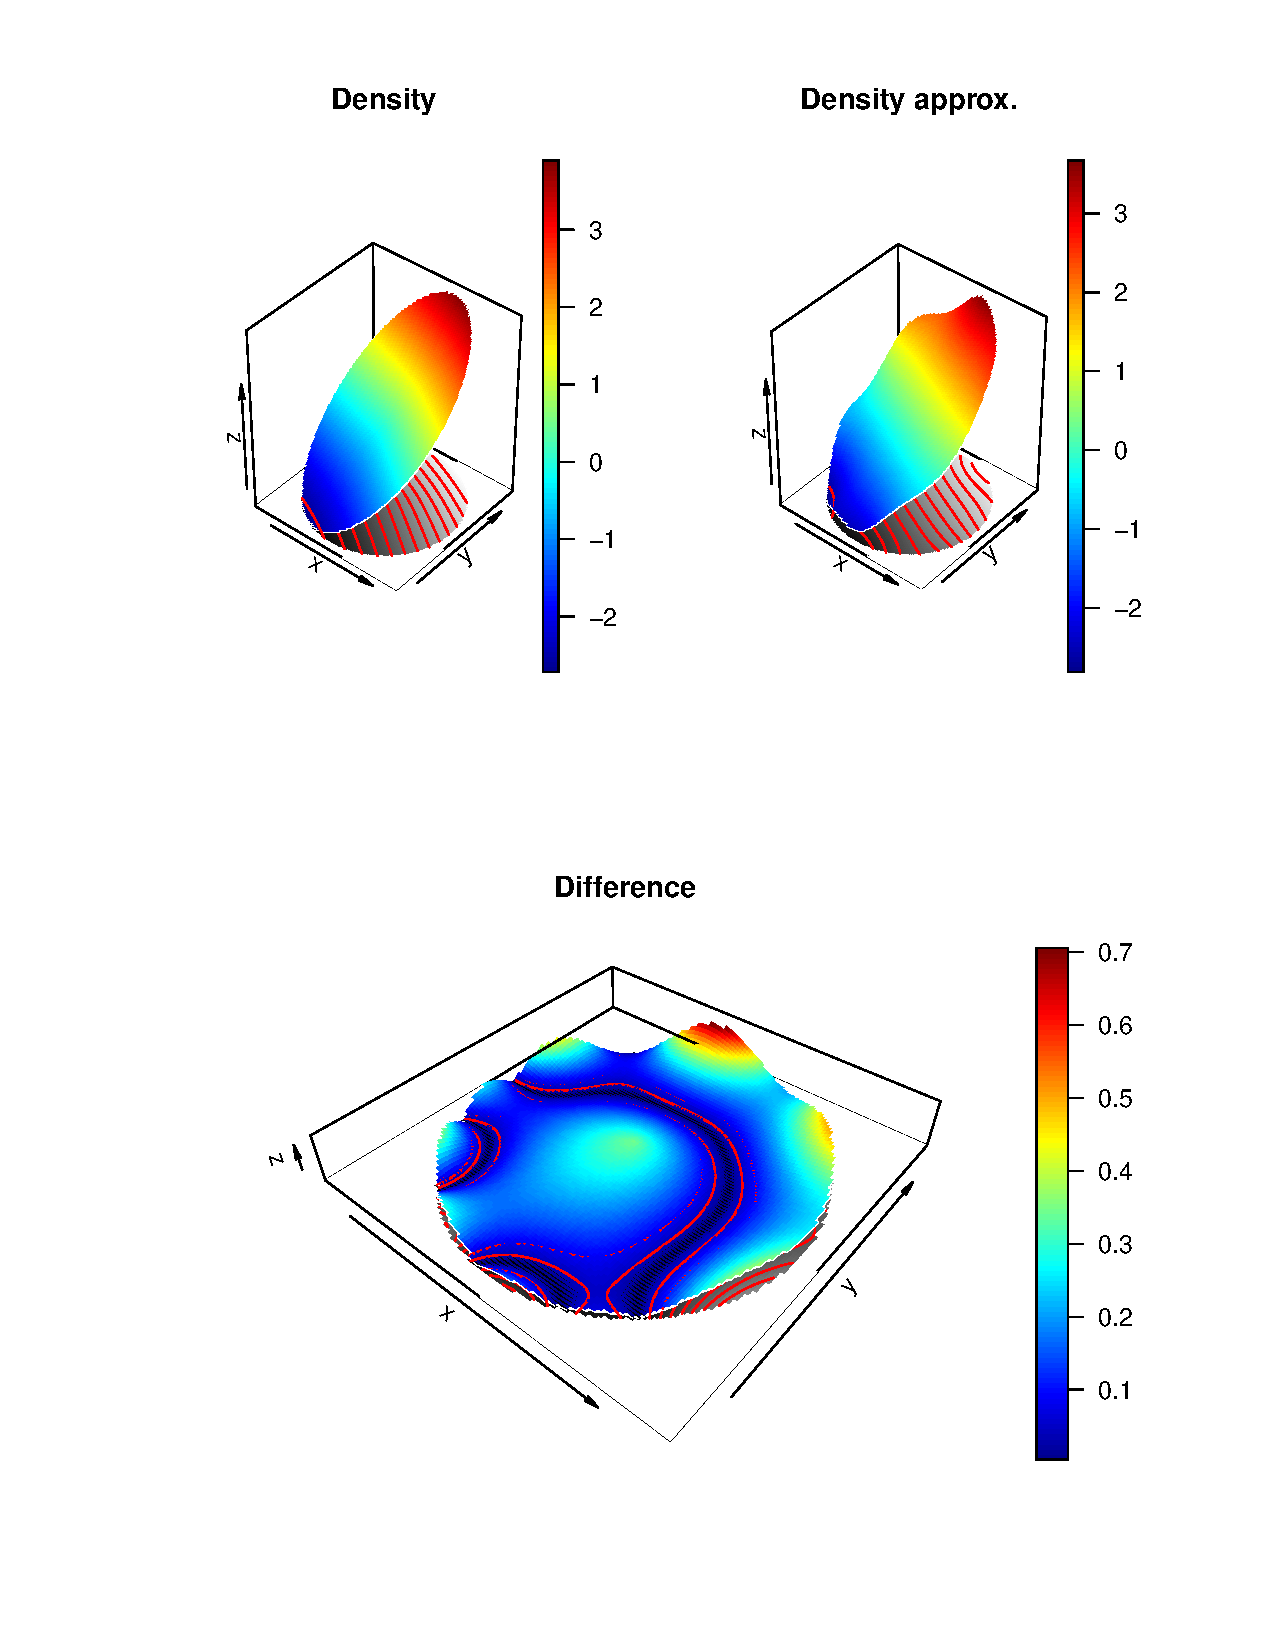
\includegraphics[width=0.95\linewidth]{f31.pdf}}
      \end{minipage}
      \hfill
      \begin{minipage}[h]{0.49\linewidth}
      \center{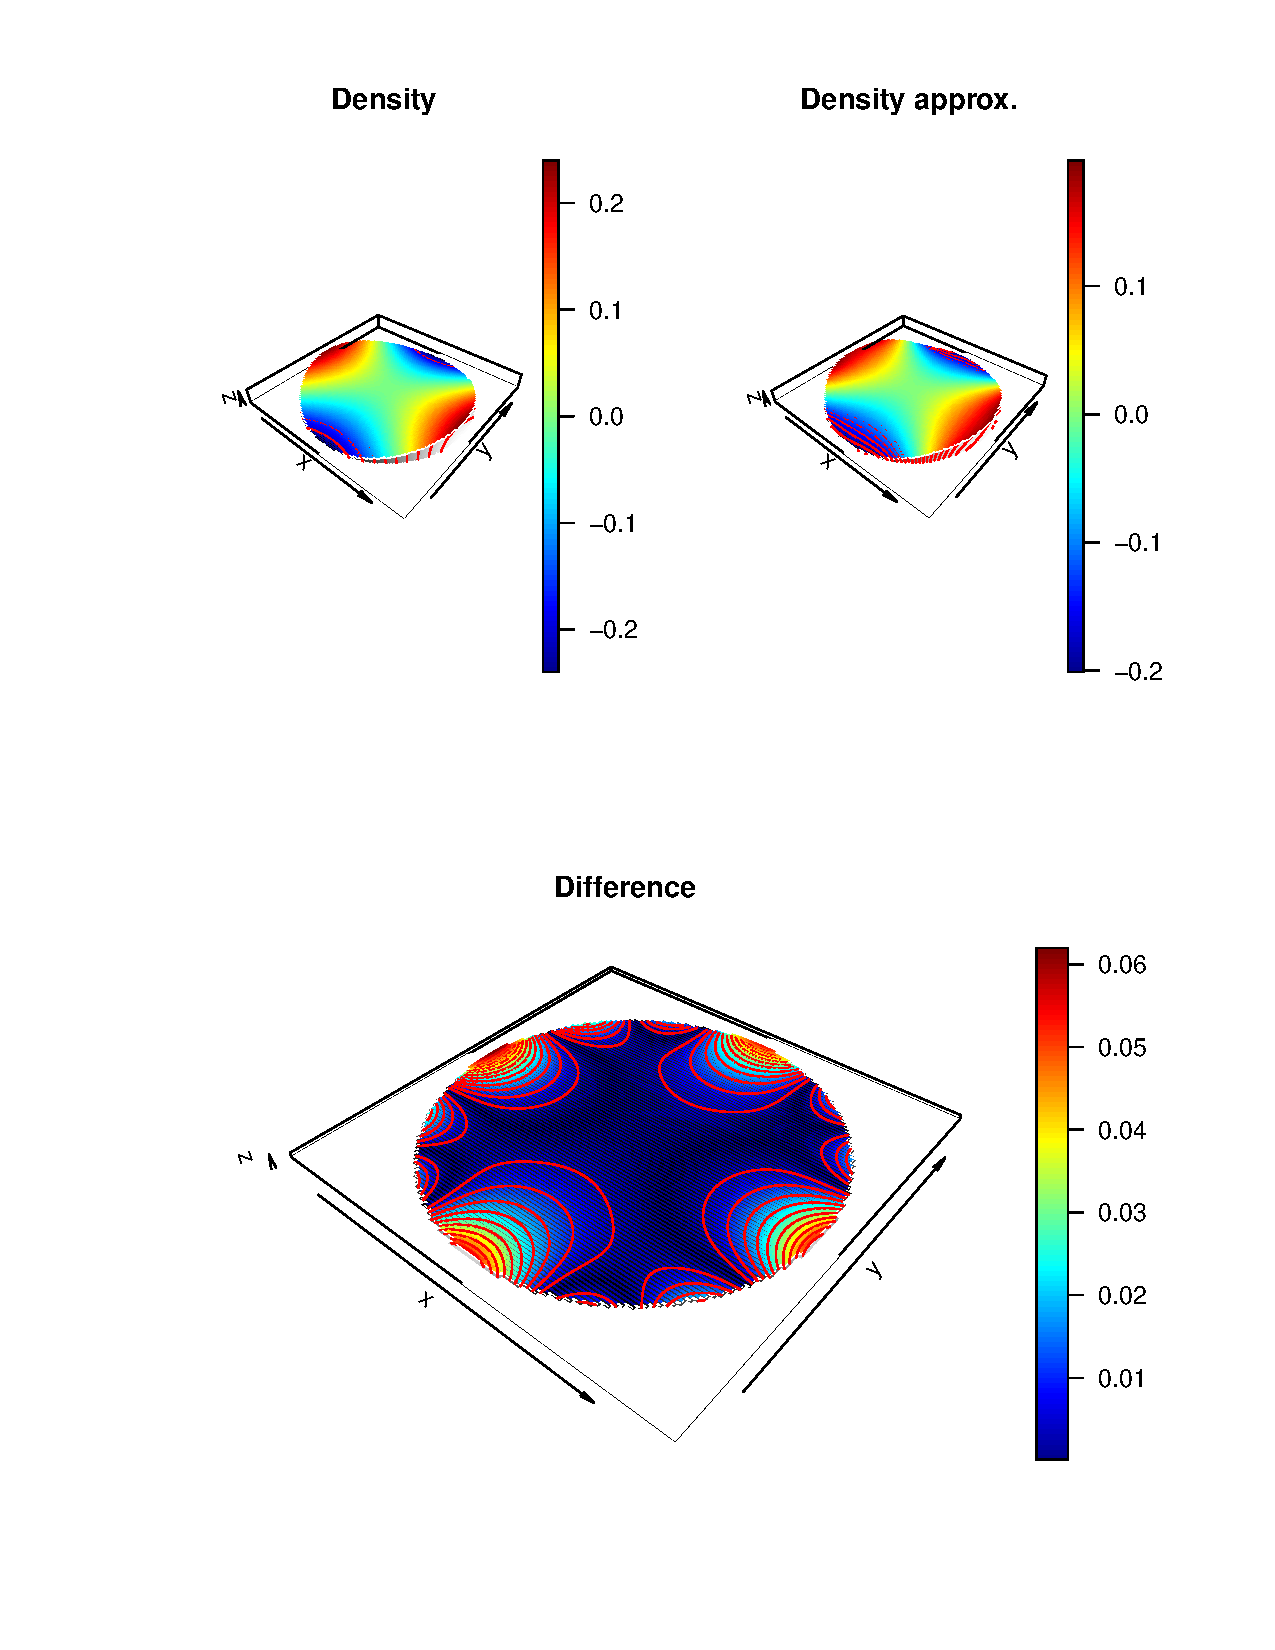
\includegraphics[width=0.95\linewidth]{f51.pdf}}
      \end{minipage}
      \caption{Для $f_3$ и $f_5$}
      \label{ris:image1}
      \end{figure}

    \begin{figure}[h]
      \begin{minipage}[h]{0.49\linewidth}
      \center{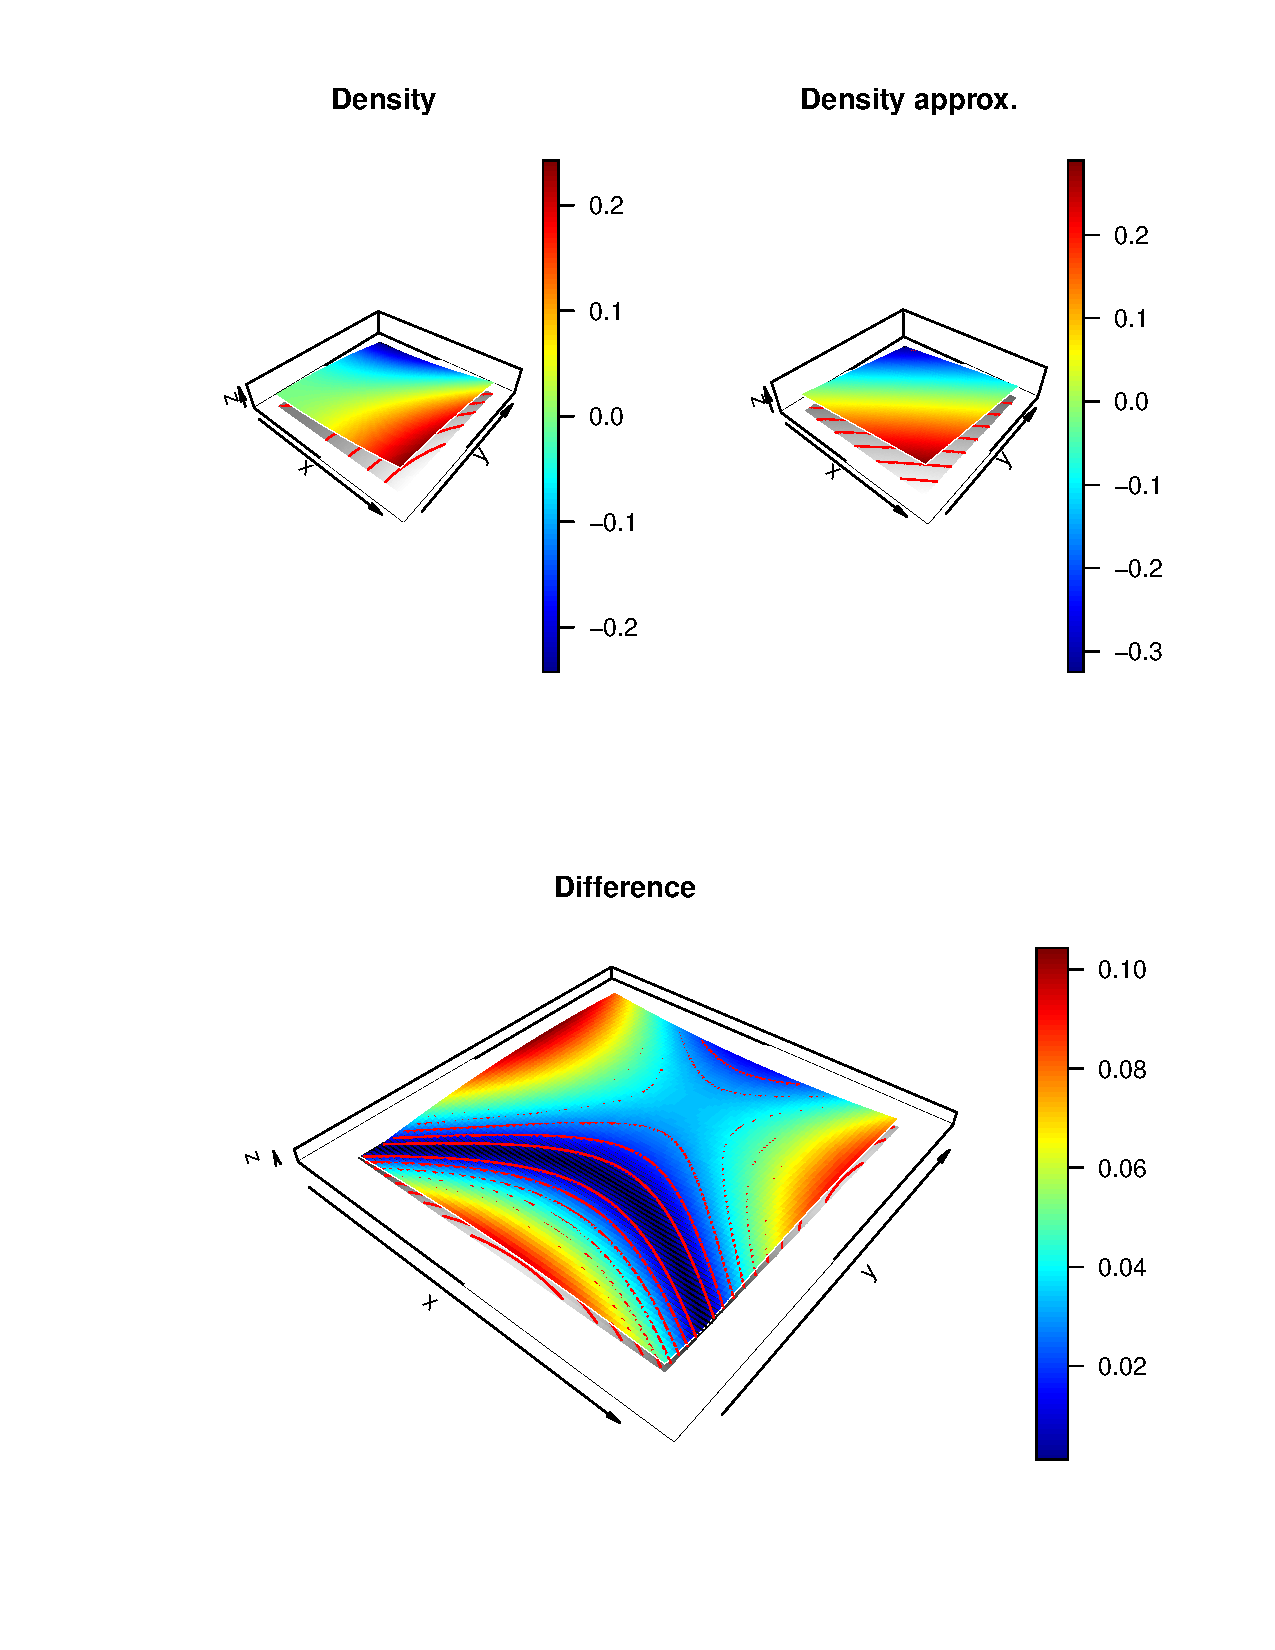
\includegraphics[width=0.95\linewidth]{f53.pdf}}
      \end{minipage}
      \hfill
      \begin{minipage}[h]{0.49\linewidth}
      \center{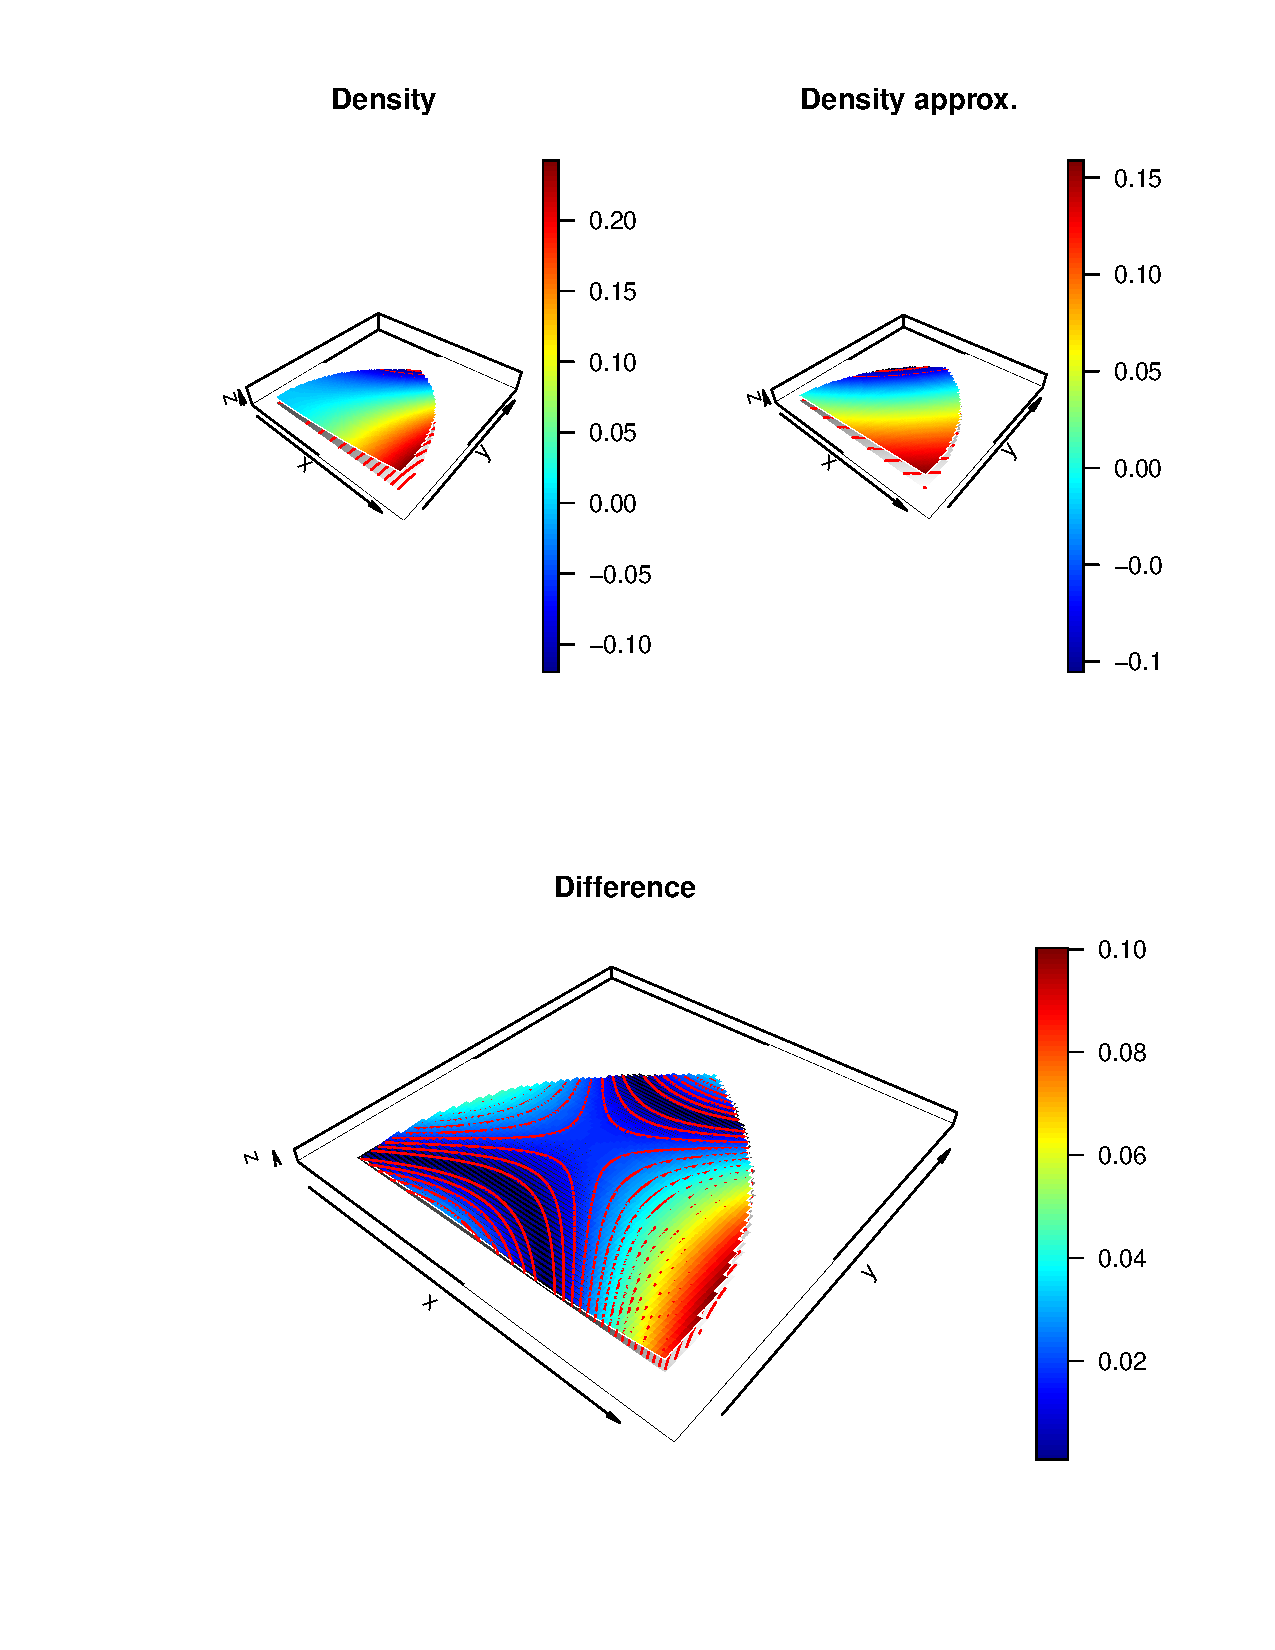
\includegraphics[width=0.95\linewidth]{f54.pdf}}
      \end{minipage}
      \caption{Для $f_5$}
      \label{ris:image1}
      \end{figure}

      \begin{figure}[h]
        \begin{minipage}[h]{0.49\linewidth}
        \center{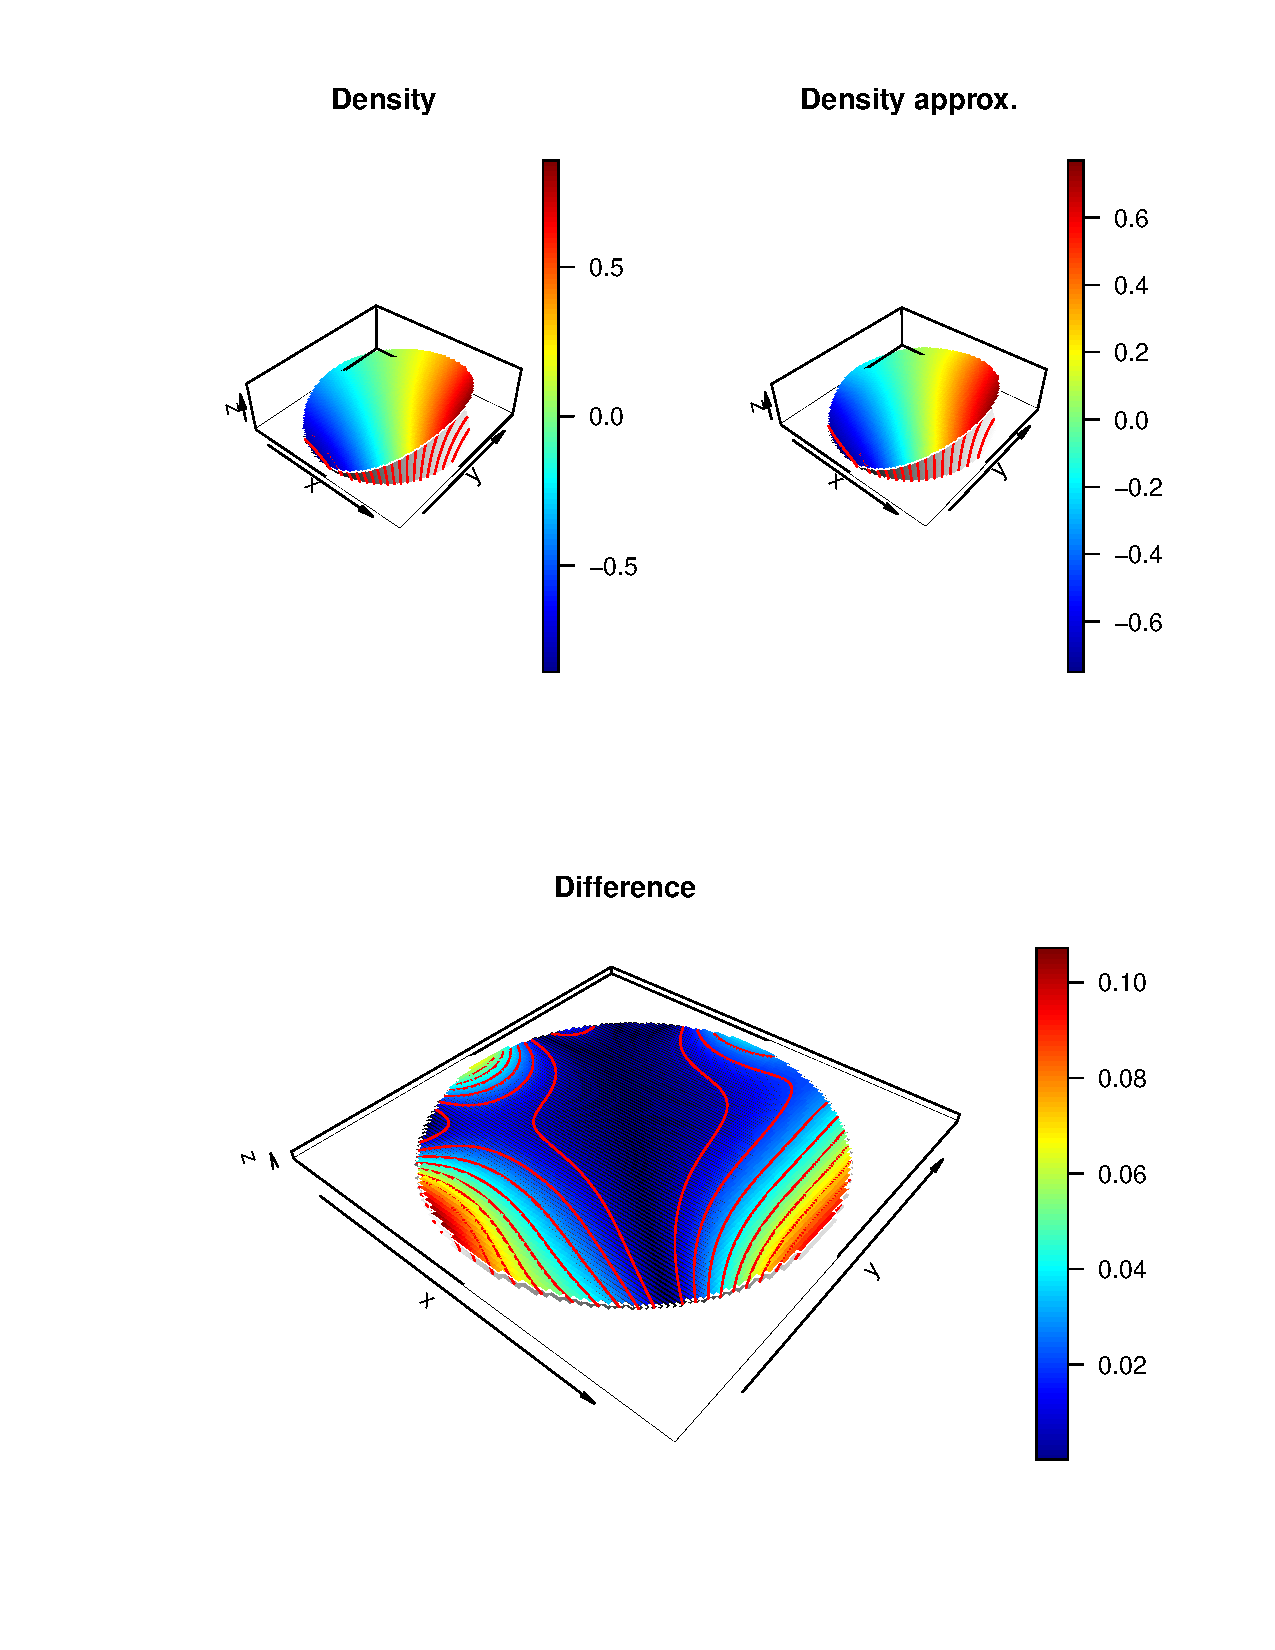
\includegraphics[width=0.95\linewidth]{f61.pdf}}
        \end{minipage}
        \hfill
        \begin{minipage}[h]{0.49\linewidth}
        \center{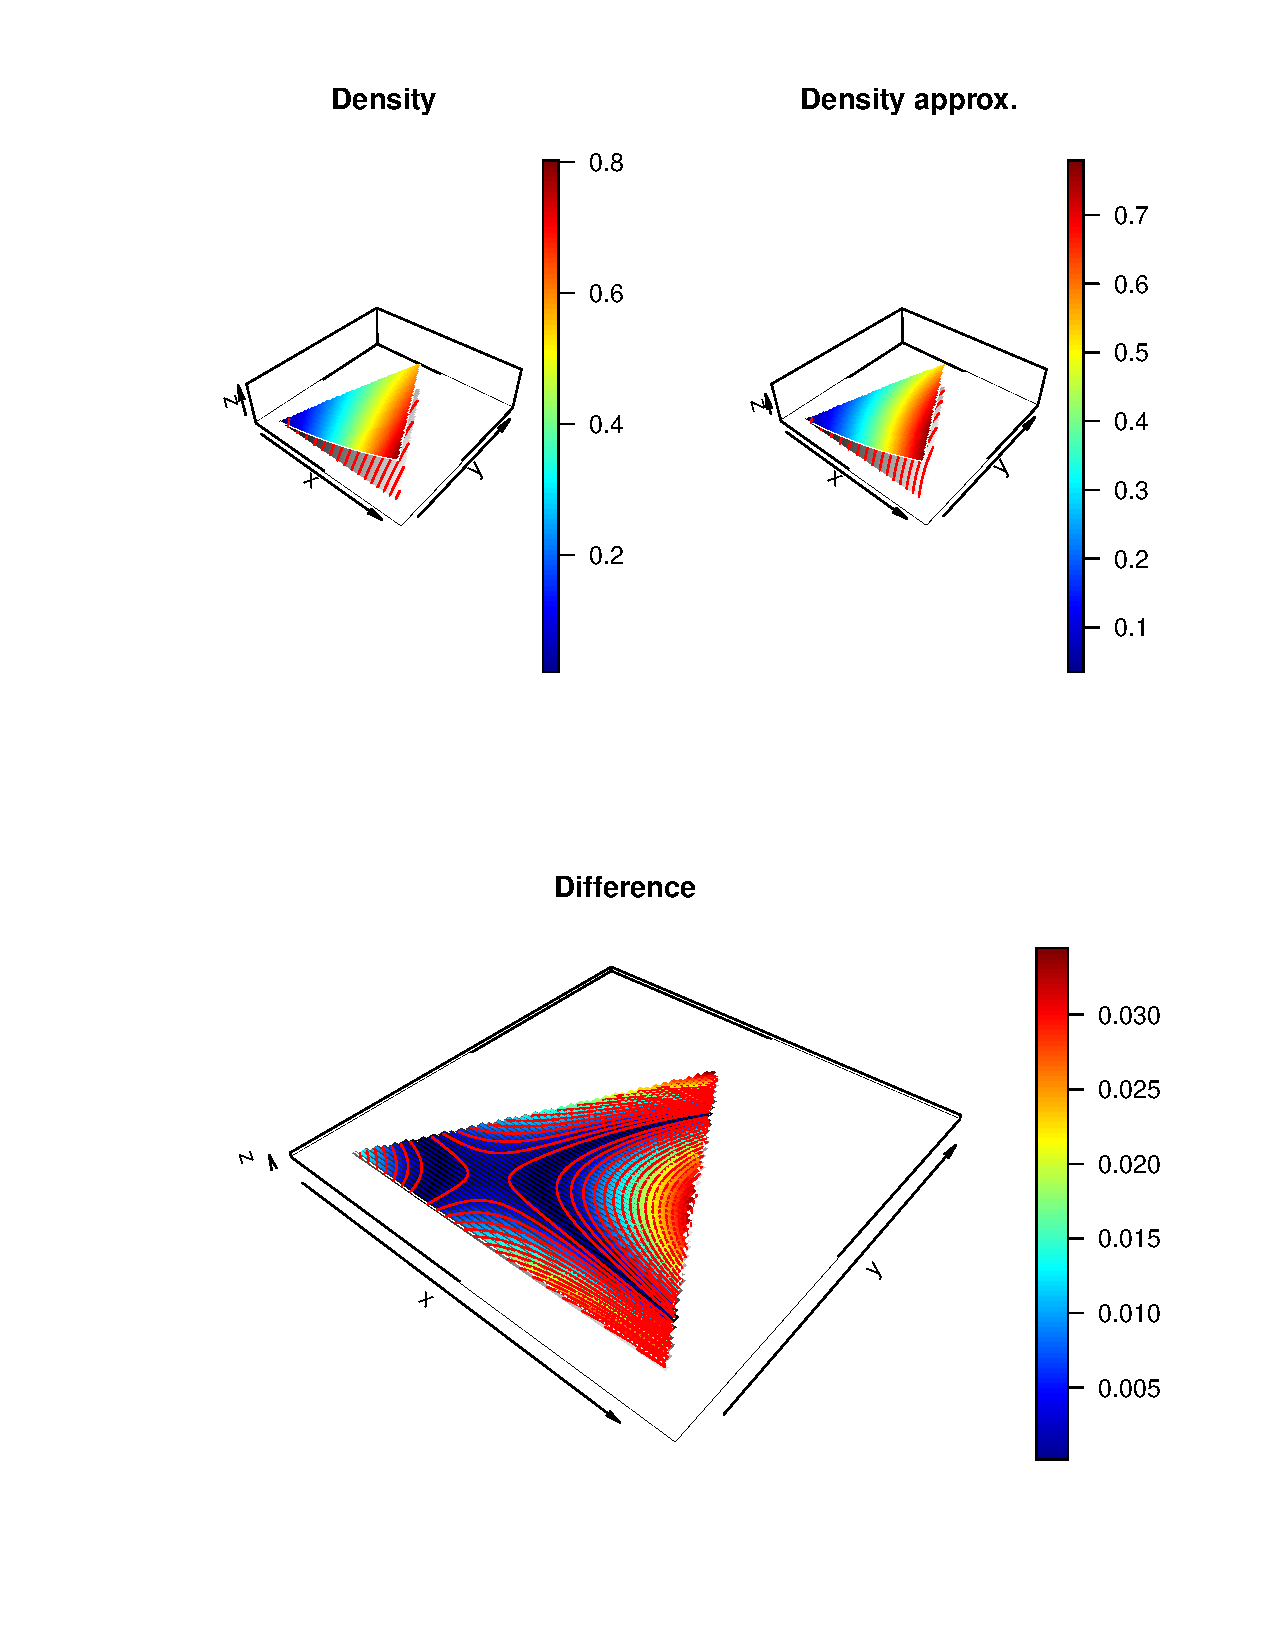
\includegraphics[width=0.95\linewidth]{f62.pdf}}
        \end{minipage}
        \caption{Для $f_6$}
        \label{ris:image1}
        \end{figure}

        \begin{figure}[h]
          \begin{minipage}[h]{0.49\linewidth}
          \center{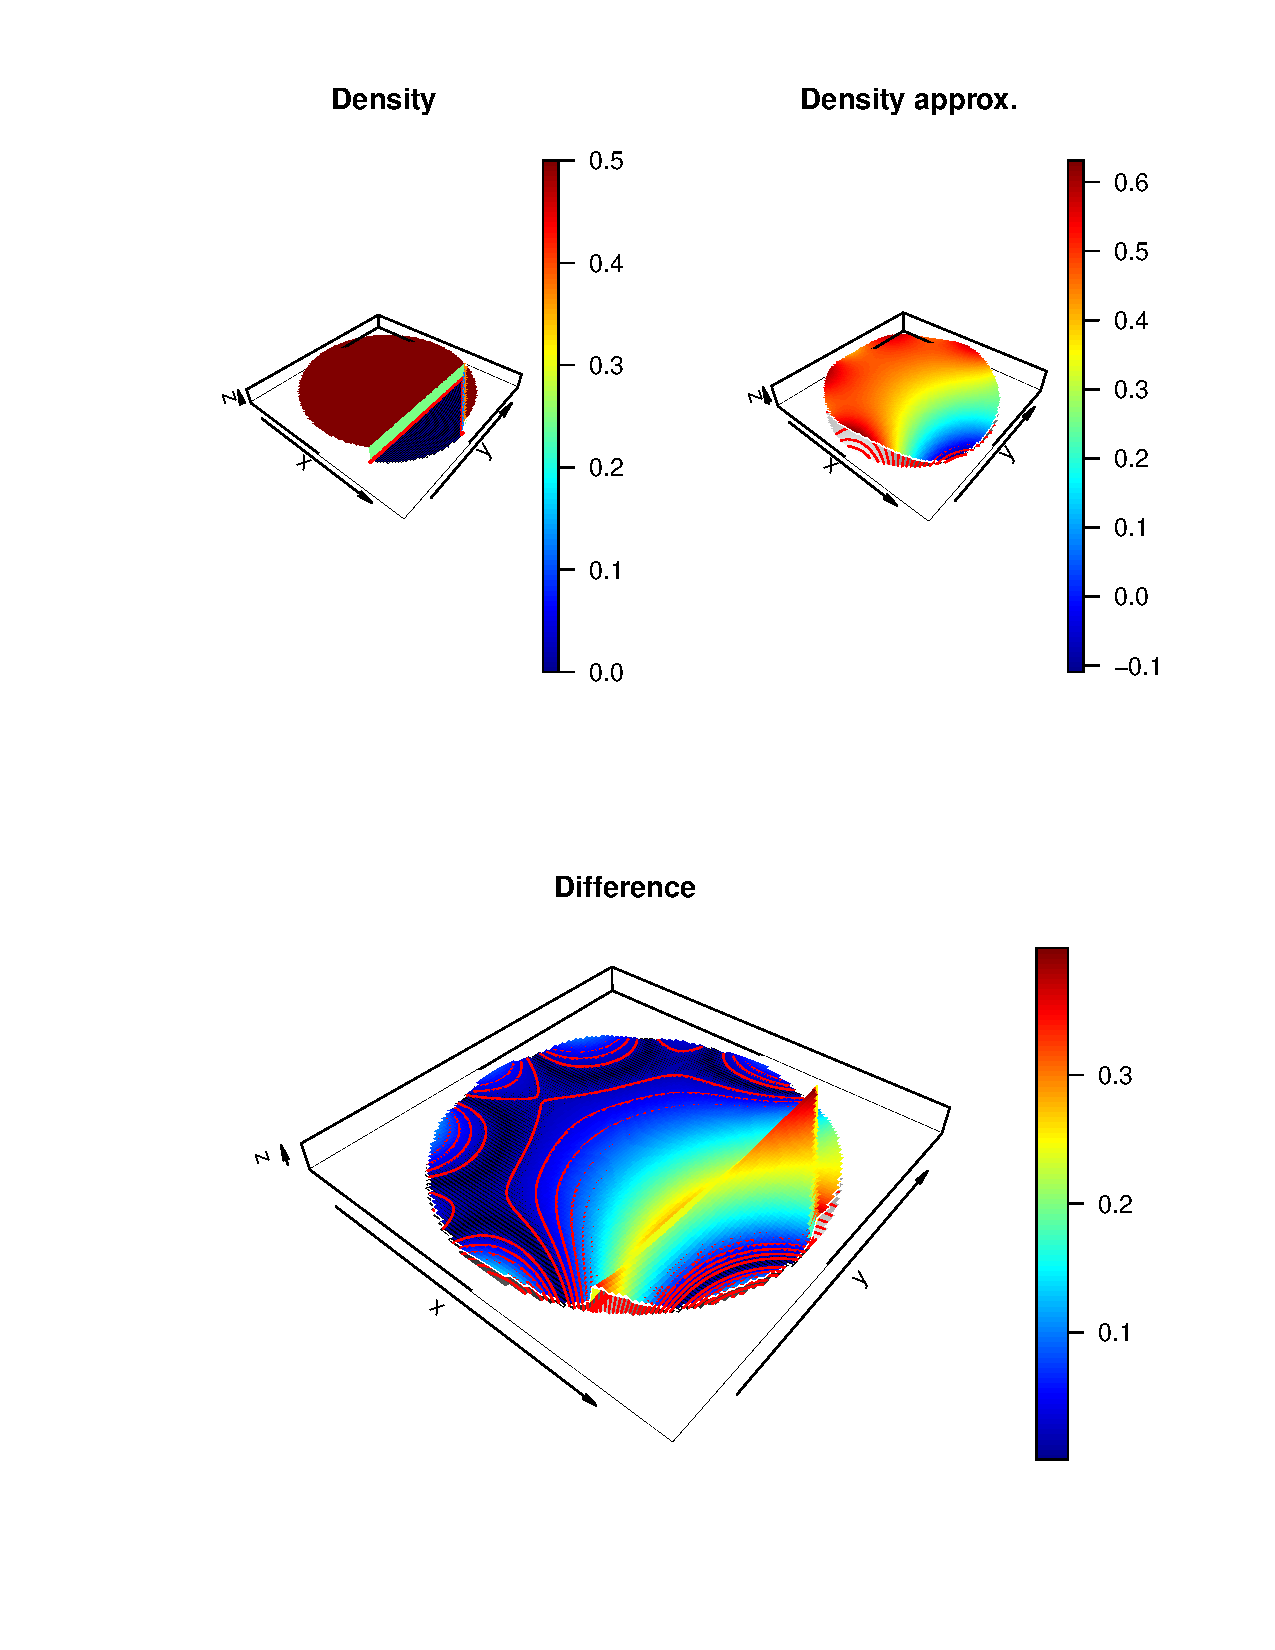
\includegraphics[width=0.95\linewidth]{f71.pdf}}
          \end{minipage}
          \hfill
          \begin{minipage}[h]{0.49\linewidth}
          \center{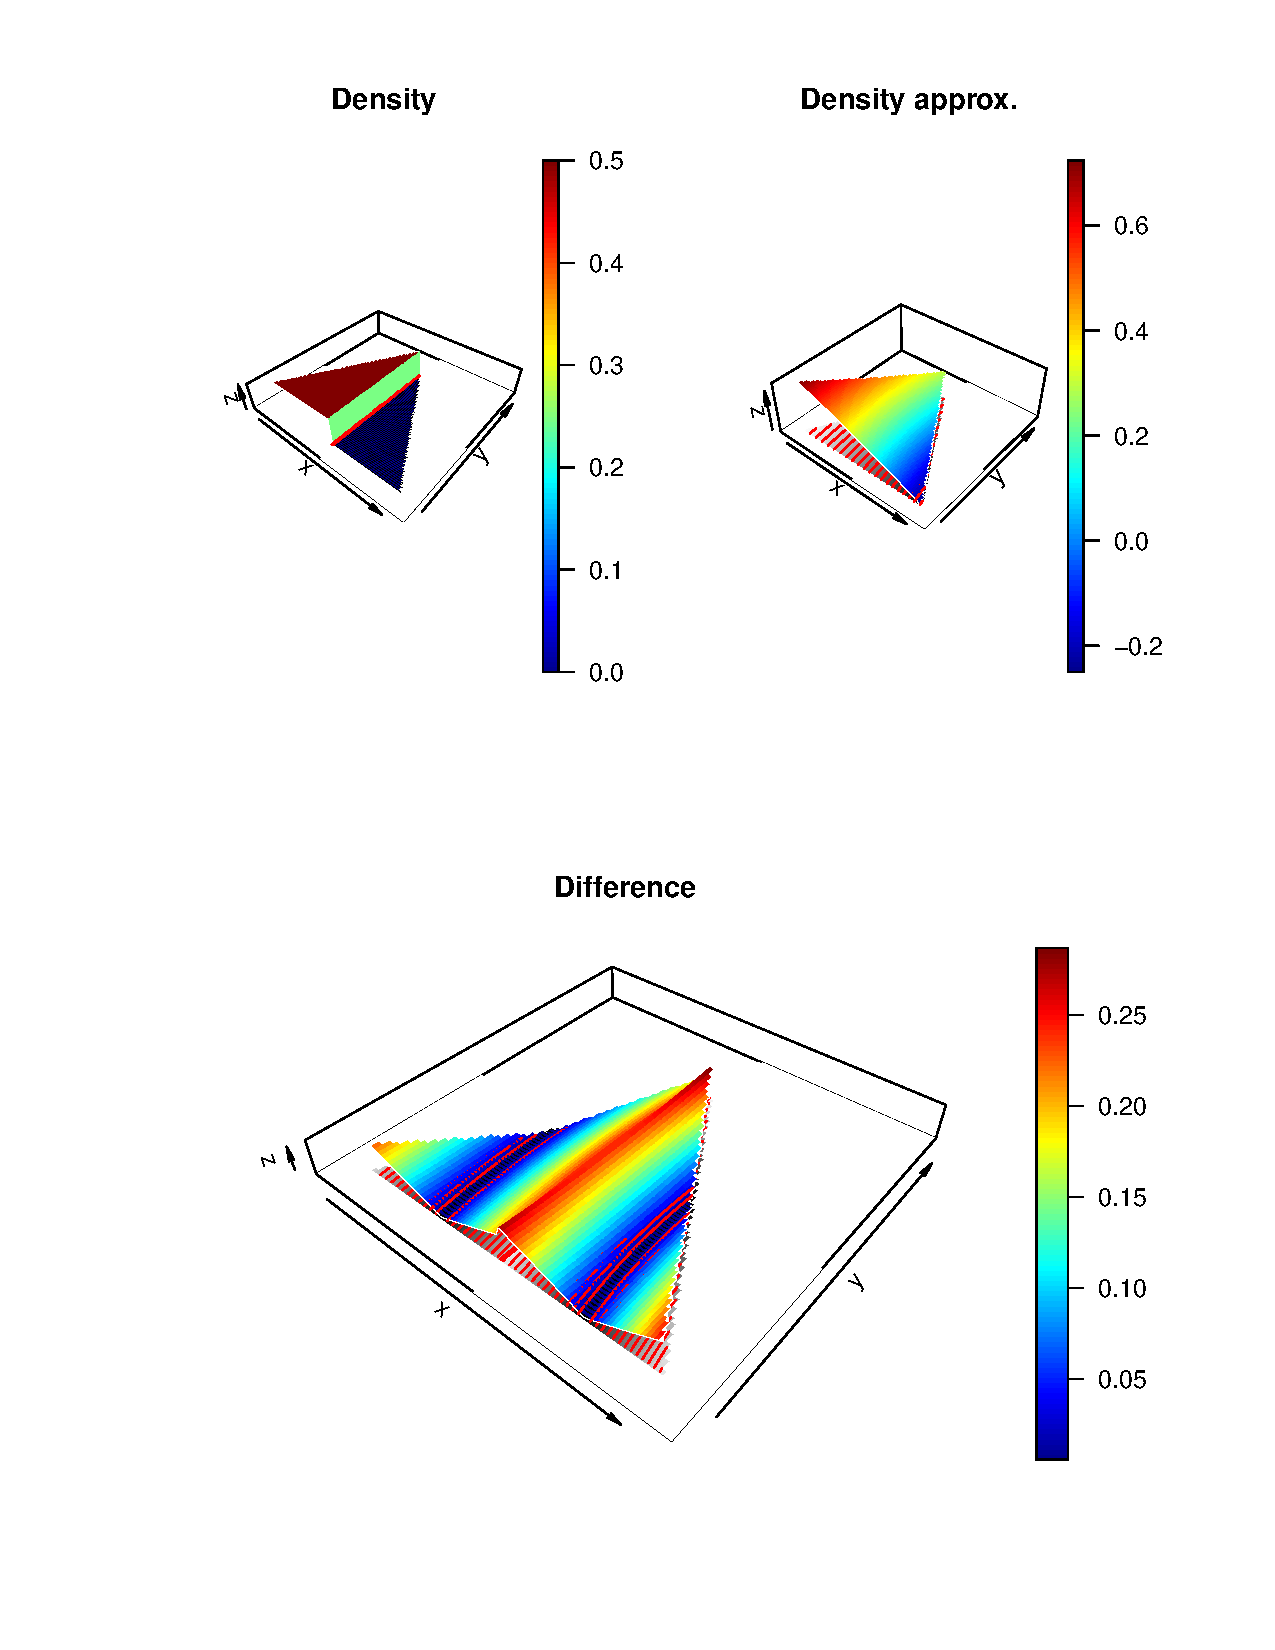
\includegraphics[width=0.95\linewidth]{f72.pdf}}
          \end{minipage}
          \caption{Для $f_7$}
          \label{ris:image1}
          \end{figure}

          \begin{figure}[h]
            \begin{minipage}[h]{0.49\linewidth}
            \center{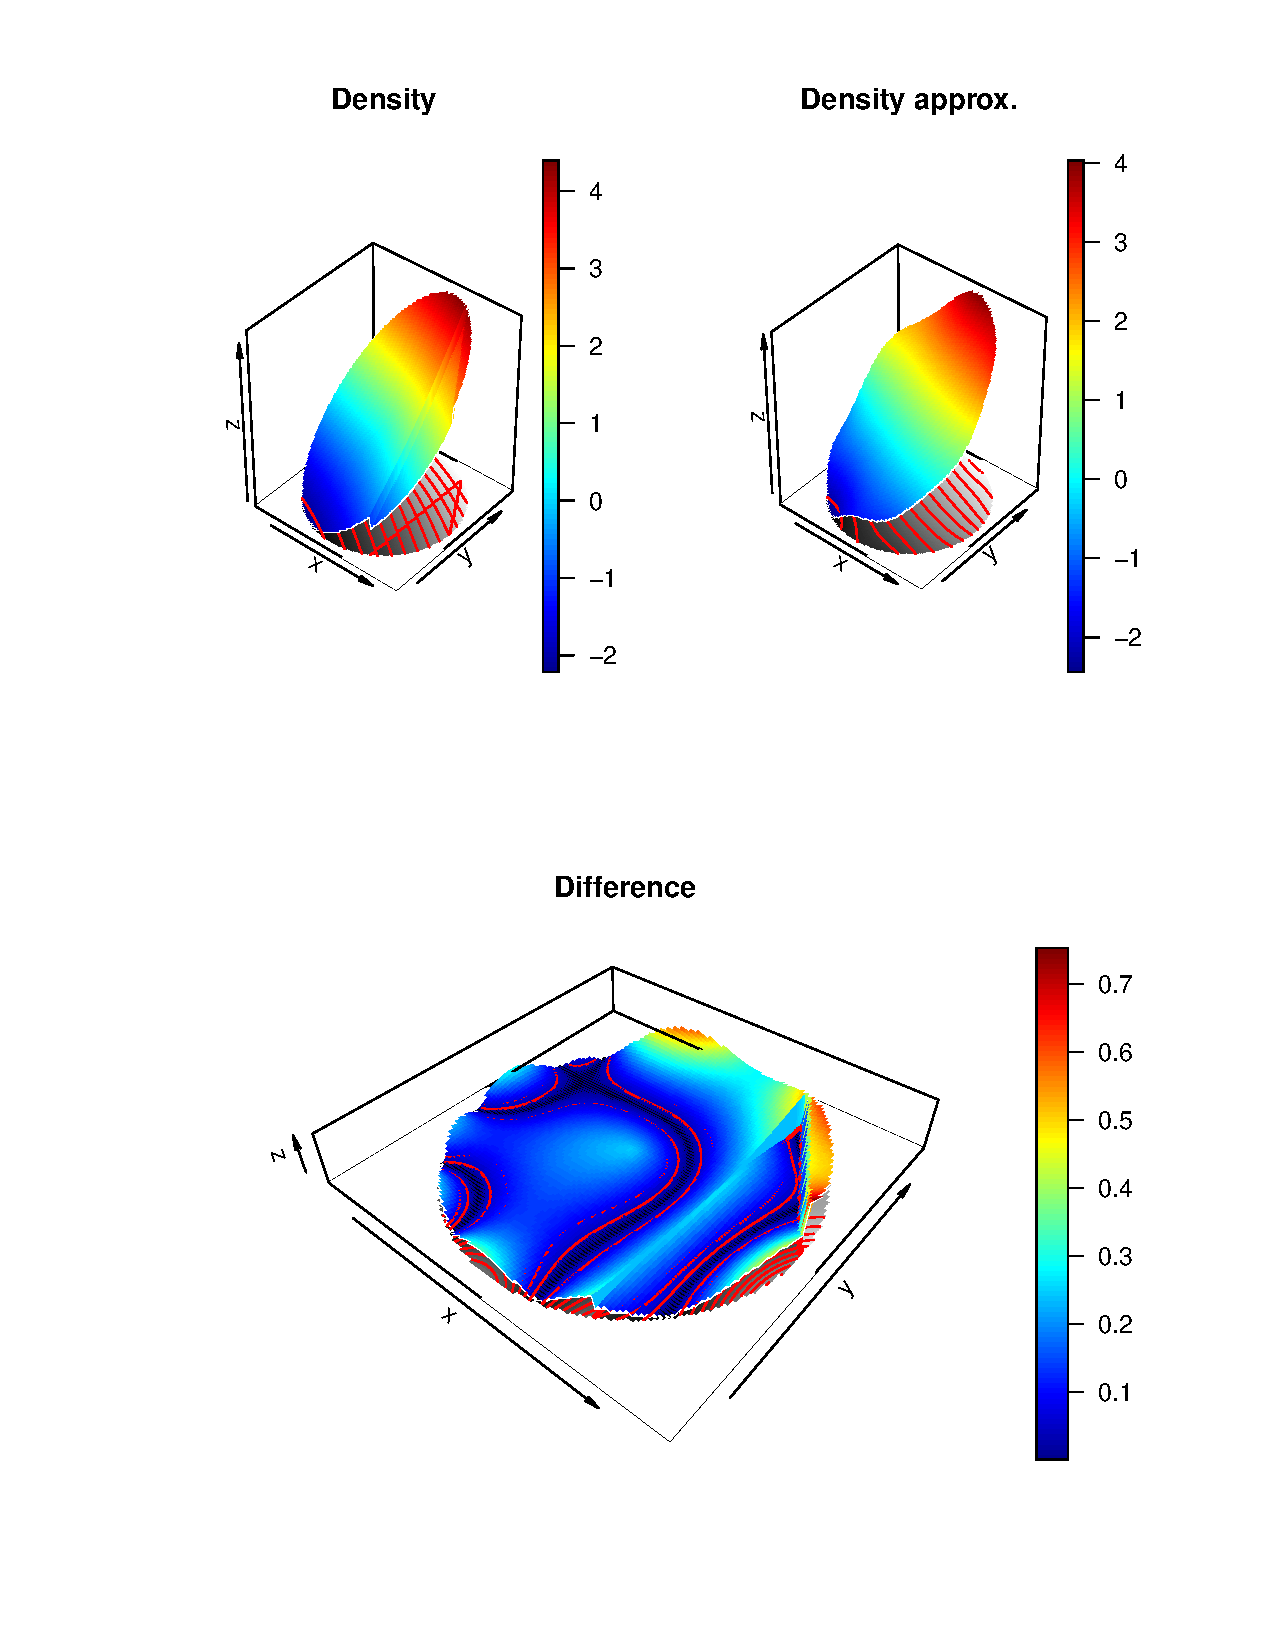
\includegraphics[width=0.95\linewidth]{f81.pdf}}
            \end{minipage}
            \hfill
            \begin{minipage}[h]{0.49\linewidth}
            \center{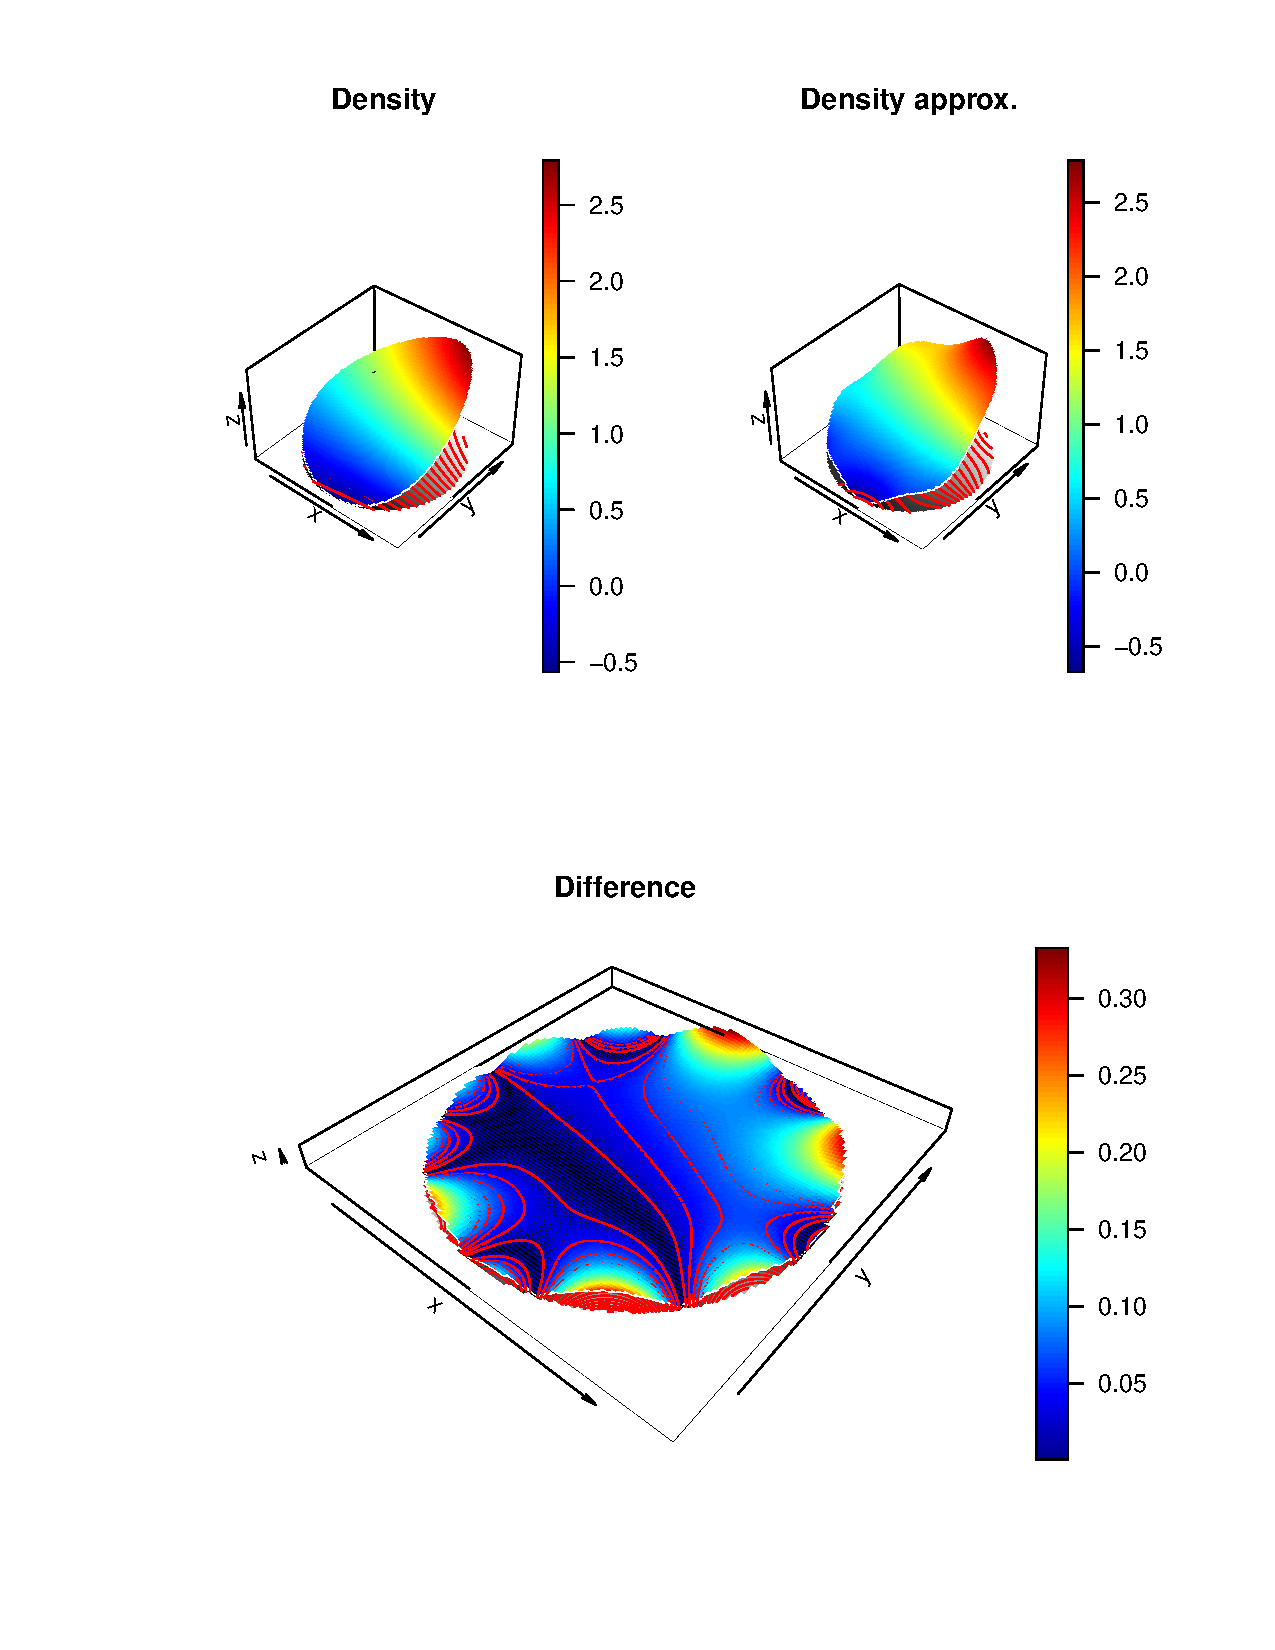
\includegraphics[width=0.95\linewidth]{f91.pdf}}
            \end{minipage}
            \caption{Для $f_8$ и $f_9$}
            \label{ris:image1}
            \end{figure}

              \begin{figure}[h]
                \begin{minipage}[h]{0.49\linewidth}
                \center{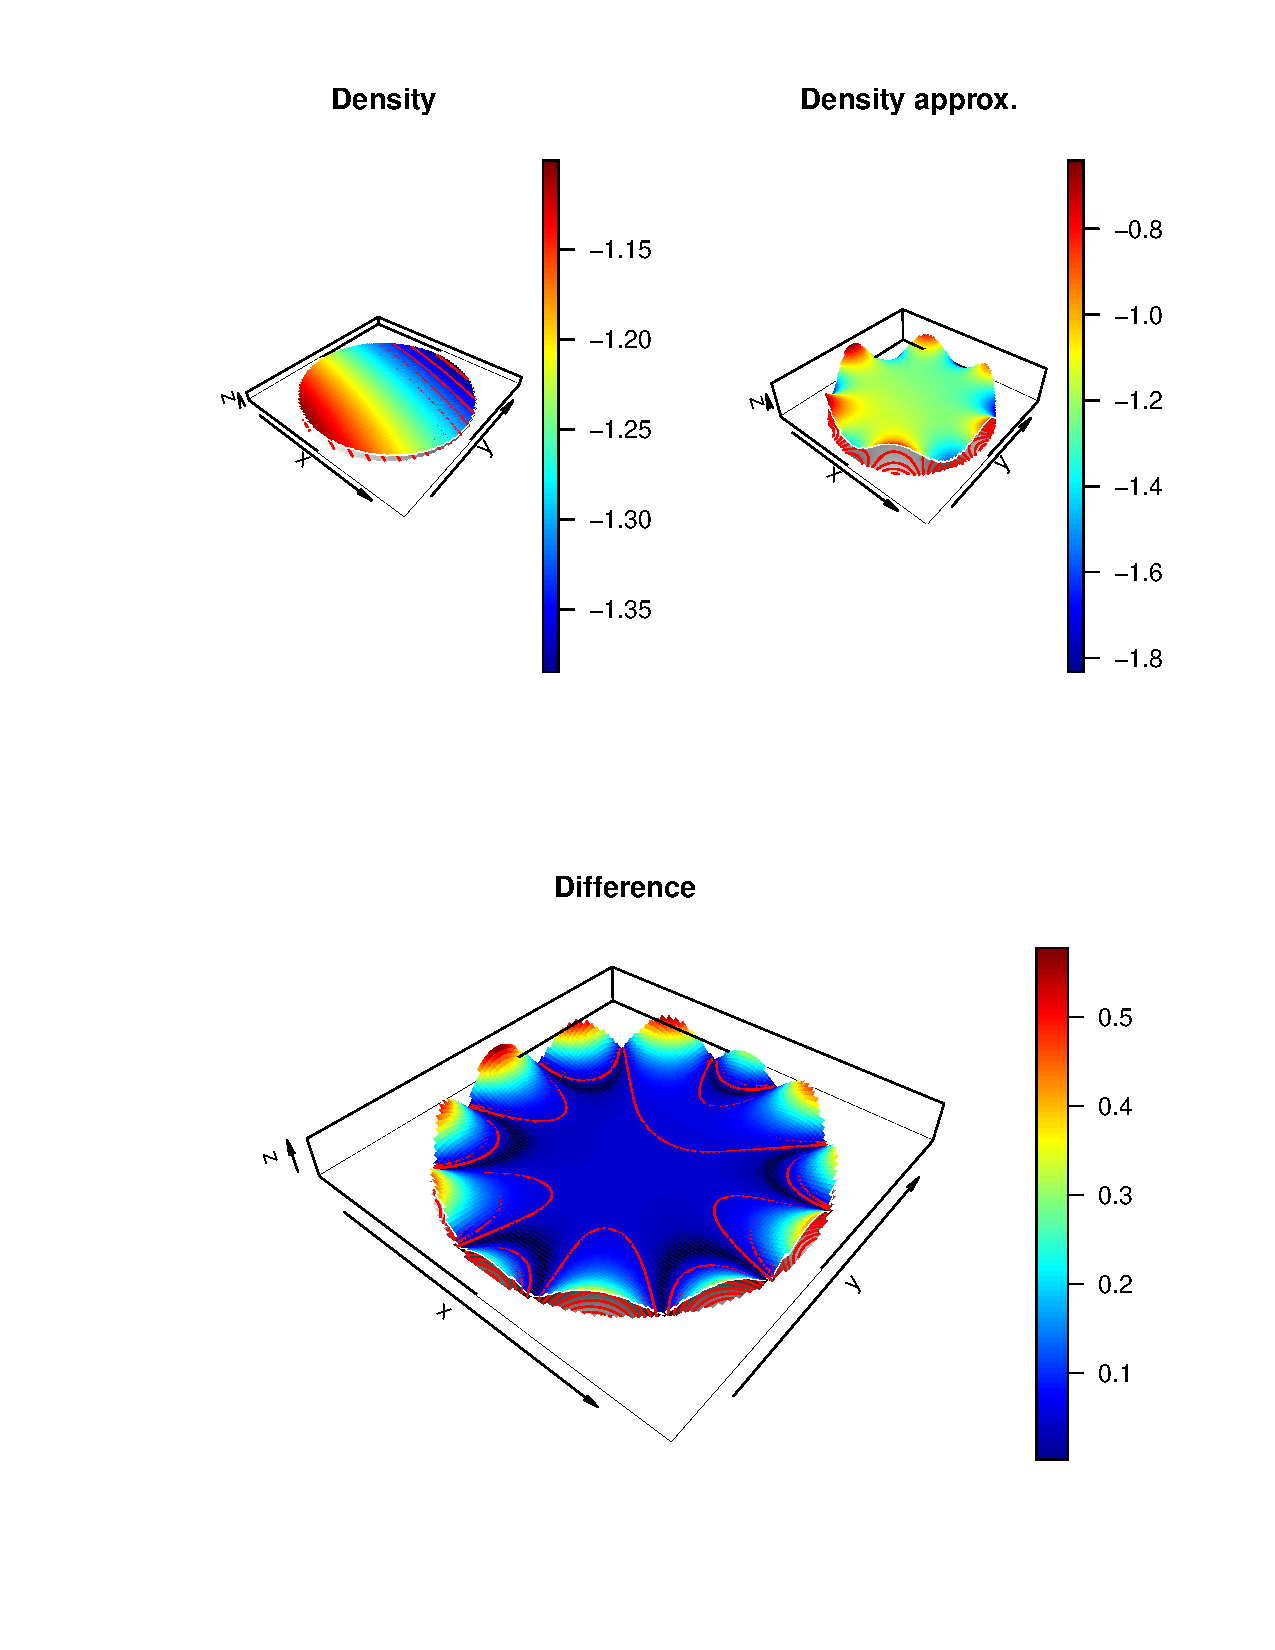
\includegraphics[width=0.95\linewidth]{f111.pdf}}
                \end{minipage}
                \hfill
                \begin{minipage}[h]{0.49\linewidth}
                \center{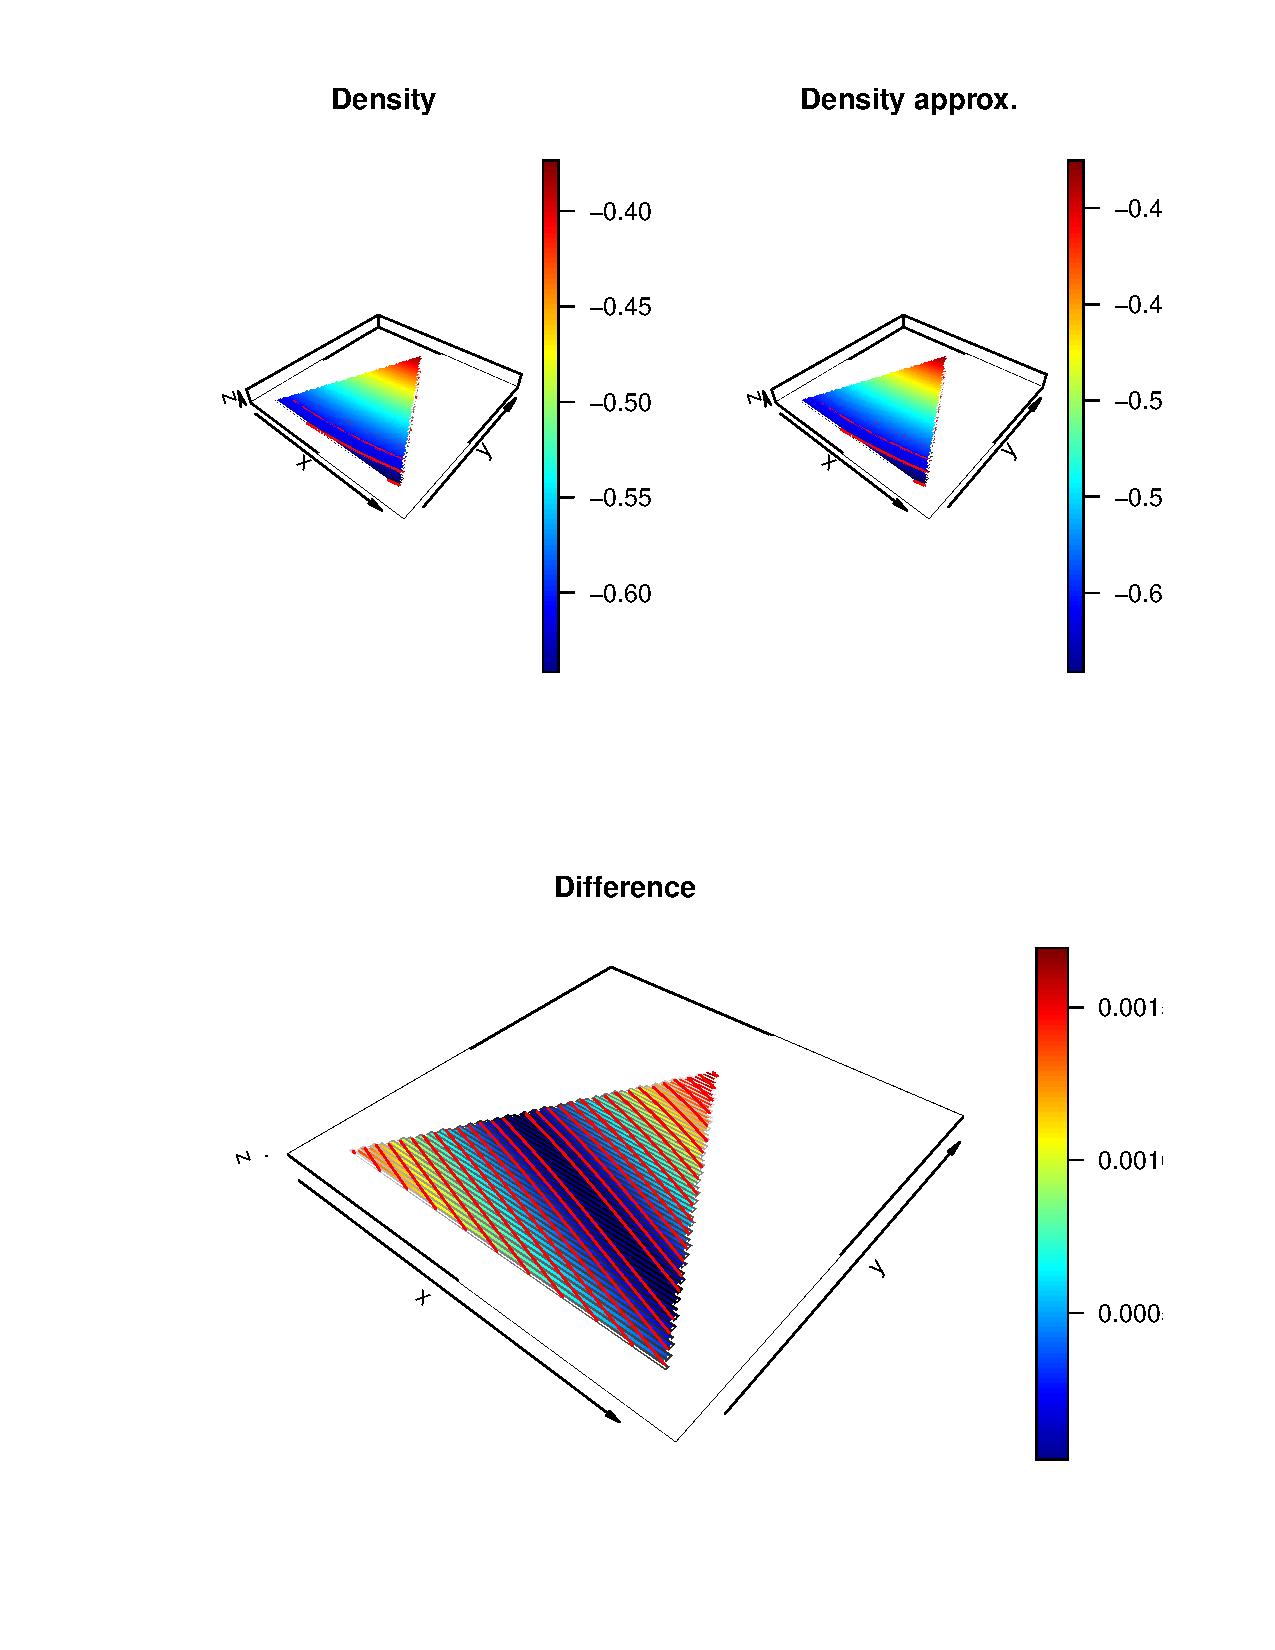
\includegraphics[width=0.95\linewidth]{f112.pdf}}
                \end{minipage}
                \caption{Для $f_{11}$}
                \label{d3end}
                \end{figure}
              

\section{Устойчивость решения ОЗГ в классе гармонических плотностей}
В этом разделе доказывается некорректность обратной задачи гравиметрии на примере системы плотностей из $\rho_k: \R{2}\rightarrow \mathbb{R}, k \in \mathbb{N}$.
Сначала показывается оценка сверху для функций $V_{\rho_k}$, затем доказывается, что $V_{\frac{\rho_k}{||\rho_k||}} \rightarrow 0, k \rightarrow 0$, затем объясняется, как это показывает некорректность ОЗГ.

\subsection{Вывод $V_{\rho_k}$}
Отождествим пока $\R{2}$ с комплексной плоскостью $\mathbb{C}$ и рассмотрим последовательность плотностей вида $\rho_k=\text{Re}\ z^k=r^k \cos k\varphi$.
Вычислим $V_{\rho_k}$ для $x=(z \cos\alpha,z \sin \alpha) \equiv z \cos\alpha + i z \sin \alpha$ вне области $Q= \{x \in \R{2}: |x|<1 \}$:
\begin{multline}
    V_{\rho_k}(x)= \int_Q \rho_k(y) E(x-y) dy= \int_0^1 \int_0^{2 \pi} r^k \cos k\varphi \ln |x-(r \cos \varphi, r \sin\varphi)| r d\varphi dr =\\
\Bigl|\alpha = \text{Arg}\ x, z=|x| \Bigl|=
\int_0^1 \int_0^{2 \pi} r^{k+1} \cos k\varphi \ln \sqrt{(z\cos \alpha-r \cos \varphi)^2+(z\sin \alpha-r \sin\varphi)^2} d\varphi dr=\\
\frac{1}{2} \int_0^1 \int_0^{2 \pi} r^{k+1} \cos k\varphi \ln(z^2 - 2z r \cos\varphi \cos \alpha +(r \cos \varphi)^2 - 2z r \sin \varphi \sin \alpha +(r \sin \varphi)^2) d\varphi dr =\\
\frac{1}{2} \int_0^1 \int_0^{2 \pi} r^{k+1} \cos k\varphi \ln(z^2-2zr(\cos \varphi \cos \alpha + \sin \varphi \sin \alpha)+r^{2})d\varphi dr=\\
\frac{1}{2} \int_0^1 r^{k+1}\int_0^{2 \pi}  \cos k\varphi \ln(z^2 + r^{2} - 2zr \cos (\varphi -\alpha)) d\varphi dr=\\
\frac{1}{2} \int_0^1 r^{k+1}\int_0^{2 \pi}\cos (k(\varphi -\alpha)+k\alpha)\ln(z^2 + r^{2} - 2zr \cos (\varphi -\alpha)) d\varphi dr= \\
\frac{1}{2} \int_0^1 r^{k+1}\int_0^{2 \pi}\left(\cos (k(\varphi -\alpha)) \cos(k\alpha) - \sin (k(\varphi -\alpha)) \sin(k\alpha)\right) \ln(z^2 + r^{2} - 2zr \cos (\varphi -\alpha)) d\varphi dr=\dots
\end{multline}

Рассмотрим интеграл $$\int_0^{2\pi} \sin (k(\varphi -\alpha)) \sin(k\alpha) \ln(z^2 + r^{2} - 2zr \cos (\varphi -\alpha)) d \varphi.$$
Поскольку функция $\sin (k(\varphi -\alpha))$ нечётна по $\varphi$, а $\cos(\varphi - \alpha)$ чётна по $\varphi$, то подинтегральная функция нечётна как произведение чётной и нечетной функций.
А поскольку $\sin (k(\varphi -\alpha))$ $ \frac{2\pi}{k}$-периодична, $k \in \mathbb{N}$, $\cos(\varphi - \alpha)$ --- $2\pi$-периодична, то указанный интеграл обращается в ноль как интеграл от нечётной периодической функции на периоде. Искомый интеграл упрощается:
\begin{multline}
   \dots =\frac{1}{2} \int_0^1 r^{k+1}\cos(k\alpha)\int_0^{2 \pi}\cos (k(\varphi -\alpha))  \ln(z^2 + r^{2} - 2zr \cos (\varphi -\alpha)) d\varphi dr=\\
   \frac{1}{2} \cos(k\alpha) \int_0^1 r^{k+1}\int_0^{2 \pi}\cos (k(\varphi -\alpha))  \ln(z^2 + r^{2} - 2zr \cos (\varphi -\alpha)) d(\varphi-\alpha) dr =\Bigl|\text{выполняем замену $\tau=\varphi - \alpha$}\Bigl|=\\
   \frac{1}{2} \cos(k\alpha) \int_0^1 r^{k+1}\int_{-\alpha}^{2 \pi - \alpha}\cos (k \tau)  \ln(z^2 + r^{2} - 2zr \cos \tau) d\tau dr =\Bigl| \text{в силу периодичности}\Bigl|=\\
   \frac{1}{2} \cos(k\alpha) \int_0^1 r^{k+1}\int_{0}^{2 \pi}\cos (k \tau)  \ln(z^2 + r^{2} - 2zr \cos \tau) d\tau dr=\\
   \frac{1}{2} \cos(k\alpha) A_k(z),
\end{multline}
где
\begin{equation}
    A_k(z)=\int_0^1 r^{k+1}\int_{0}^{2 \pi}\cos (k \tau)  \ln(z^2 + r^{2} - 2zr \cos \tau) d\tau dr.
\end{equation}

Заметим, что $A_k(z)$ ограничена:
\begin{multline}
    |A_k(z)| \leq \int_0^1 r^{k+1}\int_{0}^{2 \pi}|\cos (k \tau)|  \bigl|\ln(z^2 + r^{2} - 2zr \cos \tau)\bigl| d\tau dr \\
    \leq \int_0^1 r^{k+1}\int_{0}^{2 \pi}\bigl|\ln(z^2 + r^{2} - 2zr \cos \tau)\bigl| d\tau dr
    \leq  2\pi \int_0^1 r^{k+1} \max \left(\Bigl| \ln ((z-r)^2) \Bigl|, \Bigl| \ln ((z+r)^2) \Bigl| \right)dr \\
    \leq 2\pi \int_0^1 r^{k+1} \sup_{t \in S_r(z)} \bigl| \ln (t^2) \bigl|dr \leq 2\pi \sup_{t \in B_1(z)} \bigl| \ln (t^2) \bigl| \int_0^1 r^{k+1} dr =2\pi  \frac{\sup_{t \in B_1(z)} \bigl| \ln (t^2) \bigl|}{k+2}.
\end{multline}
Здесь под $S_r(z) \subset \mathbb{R} $ подразумевается окружность радиуса $r$ с центром в $z$, под $B_1(z) \subset \mathbb{R}$ --- шар единичного радиуса с центром в $z$. Ясно, что это сокращённое обозначение для концов отрезка $[z-r, z+r]$ и самого отрезка $[z-1,z+1]$ соответственно.

Из приведённых выкладок следует, что 
\begin{equation}
   | V_{\rho_k}(x)| \leq \pi \frac{\sup_{t \in B_1(z)} \bigl| \ln (t^2) \bigl|}{k+2},
\end{equation}
то есть для $V_{\rho_k}$ найдена оценка сверху. На рисунке \ref{chis} эта оценка подтверждается численно.
\begin{figure}[h!]
  \noindent\centering{
  \includegraphics[width=\linewidth]{valargs.pdf}
}
  \caption{Разность $\pi \frac{\sup_{t \in B_1(z)} \bigl| \ln (t^2) \bigl|}{k+2} -| V_{\rho_k}(x)| $ для разных $k$}
  \label{chis}
  \end{figure} 

\subsection{Некорректность ОЗГ}
Пусть, как и в предыдущем пункте, $Q$ --- единичный шар, а потенциал считается на поверхности $S: \{x\in \R{2}: |x|=2 \}$. В таком случае
\begin{multline}
    ||\rho_k ||_{L_2(Q)}=\sqrt{\int_0^1 \int_0^{2 \pi} r^{2k} \cos^2(k \varphi) d\varphi dr}= \sqrt{\int_0^1 r^{2k} \int_0^{2 \pi} \frac{\cos(2k \varphi)+1}{2}  d\varphi dr}\\
    =\sqrt{\frac{1}{2} \int_0^1 r^{2k} \left( \frac{\sin(2k \varphi)}{2k} +\varphi\right)\Biggl|_0^{2 \pi} dr}= \sqrt{\pi \int_0^1 r^{2k} dr}=\sqrt{\frac{\pi}{2k+1}}.
\end{multline}

Тогда
\begin{multline}
    \Bigl|\Bigl|V_{\frac{\rho_k}{||\rho_k ||}}  \Bigl|\Bigl|_{C(S)}= \frac{1}{||\rho_k ||} \Bigl|\Bigl|V_{\rho_k}  \Bigl|\Bigl|_{C(S)} \leq \sqrt{\frac{2k+1}{\pi}} \max_{x \in S} \Bigl| V_{\rho_k}(x) \Bigl| \leq \sqrt{\frac{2k+1}{\pi}} \pi |\cos(k\alpha)| \frac{\sup_{t \in B_1(2)} \bigl| \ln (t^2) \bigl|}{k+2} \\
    \leq \sqrt{\frac{2k+1}{\pi}} \pi \frac{\sup_{ t \in B_1(2)} \bigl| \ln (t^2) \bigl|}{k+2} = \sqrt{\pi} \sqrt{\frac{2k+1}{k^2 + 4k+4}}\sup_{t \in B_1(2)} \bigl| \ln (t^2) \bigl| \xrightarrow{k \rightarrow \infty} 0.
\end{multline}

Итак, доказано, что $$\Bigl|\Bigl|V_{\frac{\rho_k}{||\rho_k ||}}  \Bigl|\Bigl|_{C(S)}\xrightarrow{k \rightarrow \infty} 0.$$
Представим $V$ как линейный оператор: $V: L_2(Q) \bigcap G(Q) \rightarrow C(S)$. Пусть $S$ --- такая поверхность, что $\text{Ker} (V)=\{0\}$;
тогда существует обратный оператор $V^{-1}$.
Рассмотрим образ $V^{-1}$ на единичной сфере $\frac{V\left(\frac{\rho_k}{||\rho_k ||}\right)}{||V\left(\frac{\rho_k}{||\rho_k ||}\right)||}$:
\begin{equation}
  V^{-1}\left(\frac{V\left(\frac{\rho_k}{||\rho_k ||}\right)}{\Bigl|\Bigl|V\left(\frac{\rho_k}{||\rho_k ||}\right)\Bigl|\Bigl|}\right)=\frac{\frac{\rho_k}{||\rho_k ||}}{\Bigl|\Bigl|V\left(\frac{\rho_k}{||\rho_k ||}\right)\Bigl|\Bigl|} \xrightarrow{k\rightarrow \infty} \infty,
\end{equation}
поскольку $\Bigl|\Bigl|\frac{\rho_k}{||\rho_k ||}\Bigl|\Bigl|_{L_2(Q)}=1$ и $\Bigl|\Bigl|V_{\frac{\rho_k}{||\rho_k ||}}  \Bigl|\Bigl|_{C(S)}\xrightarrow{k \rightarrow \infty} 0.$.
Значит, оператор $V^{-1}$ неограничен, что и доказывает неустойчивость.

\section{Демонстрация некорректности}
В этом разделе будут показаны примеры из практики, демонстрирующие неустойчивость ОЗГ.
\subsection{Пояснения о неустойчивости и реализации решения}
Опираясь на пояснения из раздела 4.1, зафиксируем вблизи кривой $L$ $n$ базисных потенциалов (точек).
Решив задачу минимизации функционала
\begin{equation*}
  F(c_1,\dots,c_k,\dots,c_n)=||V_{\rho}-V_{\sum_{i=1}^n c_i \alpha_i}||_{L_2(L)},
\end{equation*}
получим некоторый набор $\bar c=(c_1,\dots,c_k,\dots,c_n)$ и значение погрешности $\varepsilon_n = \varepsilon (\bar c)$.
Ясно, что $\varepsilon$ должна не возрастать с ростом $n$, но только если рост $n$ происходит за счёт добавления новых точек в исходных набор базисных потенциалов (рисунок \ref{points2}),
поскольку разные точки вносят разный вклад в качество аппроксимации.
\begin{figure}[h!]
  \noindent\centering{
  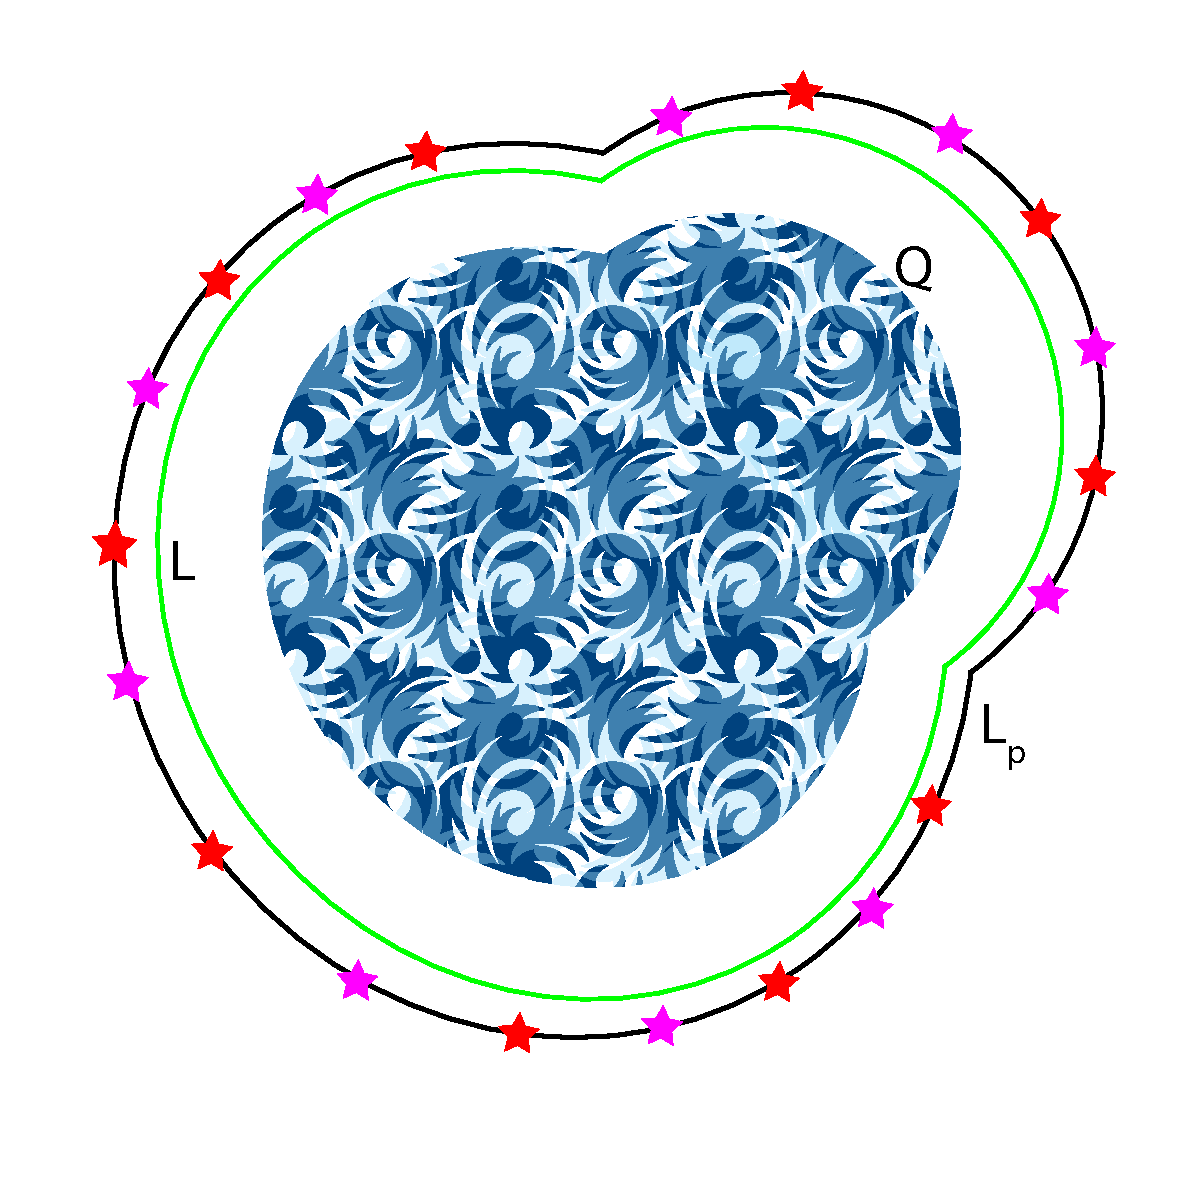
\includegraphics[width=0.7\linewidth]{Points2.pdf}
}
  \caption{С ростом числа точек аппроксимация должна не ухудшаться, если только точки добавляются к уже зафиксированным}
  \label{points2}
  \end{figure} 

Если же при каждом новом $n$ все точки пересчитываются, мы имеем дело уже с разными задачами, чьи результаты не подходят для сравнения.

Чтобы обеспечить выполнение указанного условия, я изначально фиксировал вблизи кривой максимальное количество $n$ нужных для эксперимента точек,
затем случайным образом смешивал их индексы, чтобы точки, взятые по порядку, располагались не рядом друг с другом на кривой.
После этого сразу заполнялась система $n \times n$, причём для функций $\omega_i(x) =\V{\alpha_i}, i=1,\dots,n$ производилась мемоизация (запоминание результатов), что ускоряло заполнение системы в десятки раз, так как
фактически требовалось найти лишь $n$ элементов вместо $n(n-1)$.
Далее к уже готовой системе применялся ультра-гибрид.

Поскольку ультра-гибрид гарантирует устойчивую аппроксимацию, действительно выполнялось условие $\varepsilon_k \geq \varepsilon_{k+1}, k=1, \dots, n-1$ (устойчива аппроксимация $V_{\rho} \text{ на } L_2(L)$), однако при подстановке коэффициентов решения $\bar c_k, k=1,\dots,n$ в функционал
\begin{equation*}
  T(\bar c_k)=\biggl|\biggl|\rho - \sum_{i=1}^k c_i \alpha_i\biggl|\biggl|_{L_2(Q)}=\epsilon_k,
\end{equation*}
условие $\epsilon_k \geq \epsilon_{k+1}, k=1, \dots, n-1$ более чем в половине случаев не выполнялось, то есть ультра-гибрид находил такие наборы коэффициентов $\bar c_k$, при которых
аппроксимация потенциала была устойчивой, а аппроксимация плотности --- нет, что и означает неустойчивость ОЗГ.
Кроме того, неустойчивость проявляется в том, что очень малые различия в начальных условиях (визуально прямые линии на графиках потенциалов --- на самом деле они содержат спуски в доли процентов) обращаются в заметные колебания на решении (скачки на графиках аппроксимации плотности). 

\subsection{Графики}
На рисунках \ref{neustbeg}-\ref{neustend} показано, как ведёт себя погрешность аппроксимации потенциала и его плотности при росте числа базисных точек, когда аппроксимация ведётся на фиксированной кривой $L$ (у $L$ зафиксирован радиус), когда аппроксимация потенциала устойчива.
Во всех примерах радиус $\partial Q$ равен 0.5, радиус $L_p$ (около которой расположены базисные точки) равен 3.5. На трёхмерных графиках показаны поверхности, демонстрирующие зависимость аппроксимации потенциала и плотности от числа точек и радиуса $L$, меняющегося от радиуса $\partial Q$ до 0.9 от радиуса $L_p$, также проведено масштабирование.

Графики приведены в логарифмической шкале. Поэтому, если на графиках пропущены значения (такие случаи встречались в 3D-графиках), это значит, что там аппроксимация достигает машинного нуля и логарифм от нуля не высчитывается (пример кривых, на которых достигнут машинный ноль на аппроксимации потенциала, представлен на рисунке \ref{nolnol}).
\begin{figure}[h] 
  \center{\begin{minipage}[h]{\linewidth} 
  \center{\includegraphics[width=0.8\linewidth]{fix1.pdf}} 
  \end{minipage}} 
  \vfill 
  \center{\begin{minipage}[h]{\linewidth} 
  \center{\includegraphics[width=0.8\linewidth]{fix_1.pdf}} 
  \end{minipage}} 
  \caption{Пример неустойчивости ОЗГ} 
  \label{neustbeg} 
\end{figure}
\begin{figure}[h] 
  \center{\begin{minipage}[h]{\linewidth} 
  \center{\includegraphics[width=0.8\linewidth]{fix2.pdf}} 
  \end{minipage}} 
  \vfill 
  \center{\begin{minipage}[h]{\linewidth} 
  \center{\includegraphics[width=0.8\linewidth]{fix_2.pdf}} 
  \end{minipage}} 
  \caption{Пример неустойчивости ОЗГ} 
  \label{ris:image1} 
\end{figure}
\begin{figure}[h] 
  \center{\begin{minipage}[h]{\linewidth} 
  \center{\includegraphics[width=0.8\linewidth]{fix4.pdf}} 
  \end{minipage}} 
  \vfill 
  \center{\begin{minipage}[h]{\linewidth} 
  \center{\includegraphics[width=0.8\linewidth]{fix_4.pdf}} 
  \end{minipage}} 
  \caption{Пример неустойчивости ОЗГ} 
  \label{ris:image1} 
\end{figure}

\begin{figure}[h!]
  \noindent\centering{
  \includegraphics[width=\linewidth]{nolnol.pdf}
}
  \caption{Кривые с нулевой аппроксимацией потенциала $V_{f_4}$ (обозначены красным). Обычные кривые обозначены зелёным, желтым цветом обозначена $\partial Q$. Важно отметить, что нулевая аппроксимация потенциала не приводит к нулевой аппроксимации плотности и вообще не сказывается на аппроксимации плотности как-то особенно}
  \label{nolnol}
  \end{figure} 

  \begin{figure}[h!]
    \noindent\centering{
    \includegraphics[width=0.9\linewidth]{f11d.pdf}
  }
    \caption{Зависимость аппроксимации от радиуса $L$ и числа базисных потенциалов для плотности $f_1$ и области CIRCLE}
    \label{nolnol}
    \end{figure} 

    \begin{figure}[h!]
      \noindent\centering{
      \includegraphics[width=0.9\linewidth]{f13d.pdf}
    }
      \caption{Зависимость аппроксимации от радиуса $L$ и числа базисных потенциалов для плотности $f_1$ и области TRIANGLE}
      \label{nolnol}
      \end{figure}  

      \begin{figure}[h!]
        \noindent\centering{
        \includegraphics[width=0.9\linewidth]{f21d.pdf}
      }
        \caption{Зависимость аппроксимации от радиуса $L$ и числа базисных потенциалов для плотности $f_2$ и области CIRCLE}
        \label{nolnol}
        \end{figure} 
  
        \begin{figure}[h!]
          \noindent\centering{
          \includegraphics[width=0.9\linewidth]{f41d.pdf}
        }
          \caption{Зависимость аппроксимации от радиуса $L$ и числа базисных потенциалов для плотности $f_4$ и области CIRCLE}
          \label{nolnol}
          \end{figure}       


          \begin{figure}[h!]
            \noindent\centering{
            \includegraphics[width=0.9\linewidth]{f51d.pdf}
          }
            \caption{Зависимость аппроксимации от радиуса $L$ и числа базисных потенциалов для плотности $f_5$ и области CIRCLE}
            \label{nolnol}
            \end{figure} 

            \begin{figure}[h!]
              \noindent\centering{
              \includegraphics[width=0.9\linewidth]{f53d.pdf}
            }
              \caption{Зависимость аппроксимации от радиуса $L$ и числа базисных потенциалов для плотности $f_5$ и области TRIANGLE}
              \label{nolnol}
              \end{figure} 


              \begin{figure}[h!]
                \noindent\centering{
                \includegraphics[width=0.9\linewidth]{f61d.pdf}
              }
                \caption{Зависимость аппроксимации от радиуса $L$ и числа базисных потенциалов для плотности $f_6$ и области CIRCLE}
                \label{nolnol}
                \end{figure} 

                \begin{figure}[h!]
                  \noindent\centering{
                  \includegraphics[width=0.9\linewidth]{f63d.pdf}
                }
                  \caption{Зависимость аппроксимации от радиуса $L$ и числа базисных потенциалов для плотности $f_6$ и области TRIANGLE}
                  \label{nolnol}
                  \end{figure} 

                  \begin{figure}[h!]
                    \noindent\centering{
                    \includegraphics[width=0.9\linewidth]{f71d.pdf}
                  }
                    \caption{Зависимость аппроксимации от радиуса $L$ и числа базисных потенциалов для плотности $f_7$ и области CIRCLE}
                    \label{nolnol}
                    \end{figure} 

                    \begin{figure}[h!]
                      \noindent\centering{
                      \includegraphics[width=0.9\linewidth]{f104d.pdf}
                    }
                      \caption{Зависимость аппроксимации от радиуса $L$ и числа базисных потенциалов для плотности $f_{10}$ и области EDGE}
                      \label{neustend}
                      \end{figure} 

Кроме неустойчивости ОЗГ, из рисунков можно заметить, что сам потенциал достаточно плохо аппроксимируется, когда $L$ совпадает с $L_p$ или $\partial Q$, но существует некоторая $L$ между этими двумя значениями, на которой аппроксимация будет намного лучше средней.

\section*{ }
\part{Бигармоническая задача}

\section{Постановка задачи}
Требуется найти функцию $u: \R{n} \rightarrow \mathbb{R}, u \in C(\bar{Q}) \cup D^4(Q)$, удовлетворяющую системе

\[
  \begin{cases}
\Delta^2 u=0, & \text{в $Q$} \\
\der{u}{\nu}=\varphi_1, & \text{на $\partial Q$}\\
u=\varphi_2, & \text{на $\partial Q$}
\end{cases},
\]
где $\varphi_1, \varphi_2: \partial Q \rightarrow \mathbb{R},\varphi_1, \varphi_2 \in C(\partial Q) $ --- заданные функции (\cite{samar}, стр. 422-423),
$\der{u}{\nu}=\nabla u \cdot \nu$ --- производная по нормали к области $Q$.

\section{Алгоритмы решения}
\subsection{Первый алгоритм}
Для любой функции $u \in C^2(\bar Q), Q \subset \R{n}, n \geq 2$
при любом $x \in Q$ имеет место равенство (\cite{mich}, теорема 1 на стр. 159):

\begin{equation}
   \tilde{\delta}(x) u(x)= \int_Q \Delta u(y) E(x-y) dy + \int_{\partial Q} \left(u(y)\der{E}{\nu}(x-y)-\der{u}{\nu}(y) E(x-y) \right) dy,
    \label{bg}
\end{equation}
где 
\[
    \tilde{\delta}(x) =
\begin{cases}
1, & x \in Q \\
\frac{1}{2}, & x \in \partial Q\\ 
0,& x \in Q^+ 
\end{cases}.
\]
  
Первое слагаемое является объёмным потенциалом, второе --- разностью потенциалов двойного и простого слоя соответственно.

Приближённое решение $\tilde{u}$ задачи будем искать в виде (\ref{bg}); учитывая бигармоническую задачу, оно принимает вид:
\begin{equation}
  \tilde{u}(x)= \int_Q \tilde{\rho}(y) E(x-y) dy + \int_{\partial Q} \left(\varphi_2(y)\der{E}{\nu}(x-y)-\varphi_1(y) E(x-y) \right) dy.
  \label{u1}
\end{equation}

Поскольку $\tilde{\delta}(x)=0, x \in Q^+$, то поставленная задача сводится к поиску функции $\tilde{\rho}\ \forall x \in Q^+$ из уравнения
\begin{equation}
    \int_Q \tilde{\rho}(y) E(x-y) dy + \int_{\partial Q} \left(\varphi_2(y)\der{E}{\nu}(x-y)-\varphi_1(y) E(x-y) \right) dy=0,
\end{equation} 
эквивалентного 
\begin{equation}
    \int_Q \tilde{\rho}(y) E(x-y) dy = \int_{\partial Q} \left(\varphi_1(y) E(x-y) -\varphi_2(y)\der{E}{\nu}(x-y)\right) dy.
    \label{bgogz}
\end{equation} 
Раз правая часть уравнения может быть посчитана, $\tilde{\rho}$ может быть найдено как решение уже рассмотренной ОЗГ, когда $x$ проходит по некоторой поверхности $L$.
Затем найденная плотность подставляется в выражение (\ref{u1}), в котором уже $x \in Q$.

\subsection{Второй алгоритм}

\section{Сравнение алгоритмов}

\section*{Заключение}


\begin{thebibliography}{15} 
 \bibitem{lezh}
  Задачи и алгоритмы плоскопараллельных течений: учеб. пособие / М. В. Лежнев. -- Краснодар: Кубанский гос. ун-т, 2009
\bibitem{mich}
  Михайлов В. П. Дифференциальные уравнения в частных производных. --- 2-е изд. перераб. и дополн. --- М.: Наука, главная редакция физико-математической литературы, 1983
\bibitem{samar}
  Уравнения математической физики: Учеб. пособие. --- 6-е изд., испр. и доп. --- М.: Изд-во МГУ, 1999.
\bibitem{nov}
Новиков П. С. Избранные труды. Теория множеств и функций. Математическая логика и алгебра. М.: Наука, 1979, 396 

\end{thebibliography}


\end{document}